%
%  monografia
%
%  Created by Ricardo de Cillo on 2012-05-27.
%  Copyright (c) 2012 __MyCompanyName__. All rights reserved.
%
\documentclass[a4paper,11pt]{article}

% Use utf-8 encoding for foreign characters
\usepackage[brazil]{babel}
\usepackage[utf8]{inputenc}
\usepackage[T1]{fontenc}

% Setup for fullpage use
\usepackage{fullpage}
\usepackage{setspace}

% Uncomment some of the following if you use the features
%
% Running Headers and footers
%\usepackage{fancyhdr}

% Multipart figures
%\usepackage{subfigure}

% More symbols
\usepackage{amsfonts}
\usepackage{amssymb, amsmath}
%\usepackage{latexsym}

\usepackage{morefloats}

\usepackage{multirow}

% Surround parts of graphics with box
\usepackage{boxedminipage}

% Package for including code in the document
\usepackage{listings}

% If you want to generate a toc for each chapter (use with book)
\usepackage{minitoc}

% This is now the recommended way for checking for PDFLaTeX:
\usepackage{ifpdf}

%\newif\ifpdf
%\ifx\pdfoutput\undefined
%\pdffalse % we are not running PDFLaTeX
%\else
%\pdfoutput=1 % we are running PDFLaTeX
%\pdftrue
%\fi

\ifpdf
\usepackage[pdftex]{graphicx}
\else
\usepackage{graphicx}
\fi


\usepackage{xcolor}
\newcommand{\TODO}[1]{\textcolor{red}{#1}}


%% \title{Aplicação de análise morfológica para segmentação de páginas em imagens de documentos}
%% \author{ Aluno: Ricardo de Cillo \\ Supervisora: Nina S. T. Hirata }

% \date{2012-05-27}

\begin{document}

%  \maketitle

% =======================================================================
% CAPA
% =======================================================================

\thispagestyle{empty}
\

\

\

\

\begin{center}
{\bf \Large Trabalho de Formatura Supervisionado}

\bigskip
\bigskip
{\bf \LARGE Aplicação de análise morfológica para segmentação de páginas em imagens de documentos}

\bigskip
{\large Ricardo de Cillo}

\bigskip
Supervisora: Nina S. T. Hirata 

\bigskip
Departamento de Ciência da Computação\\
Intituto de Matemática e Estatística, IME-USP
\end{center}


\bigskip
\begin{quote}
\begin{spacing}{1.2}
\noindent {\bf \large Resumo}: Neste texto apresentamos nosso estudo sobre a aplicação de operadores morfológicos à segmentação de páginas de documentos, etapa importante na análise de documentos que busca extrair informações sobre a sua estrutura: regiões com títulos, legendas, figuras e blocos de texto.
\end{spacing} 
\end{quote}

\bigskip
\begin{center}
São Paulo, \today
\end{center}


\newpage

\tableofcontents

\newpage
\setcounter{page}{1}

\section{Introdução}

Processamento e análise de documentos é uma importante subárea da área
de reconhecimento de padrões cujo principal objetivo é a
interpretação de um documento, ou seja, o entendimento
da sua estrutura bem como o reconhecimento de cada um dos
componentes estruturais.

\begin{figure*}[htb]
\begin{center}
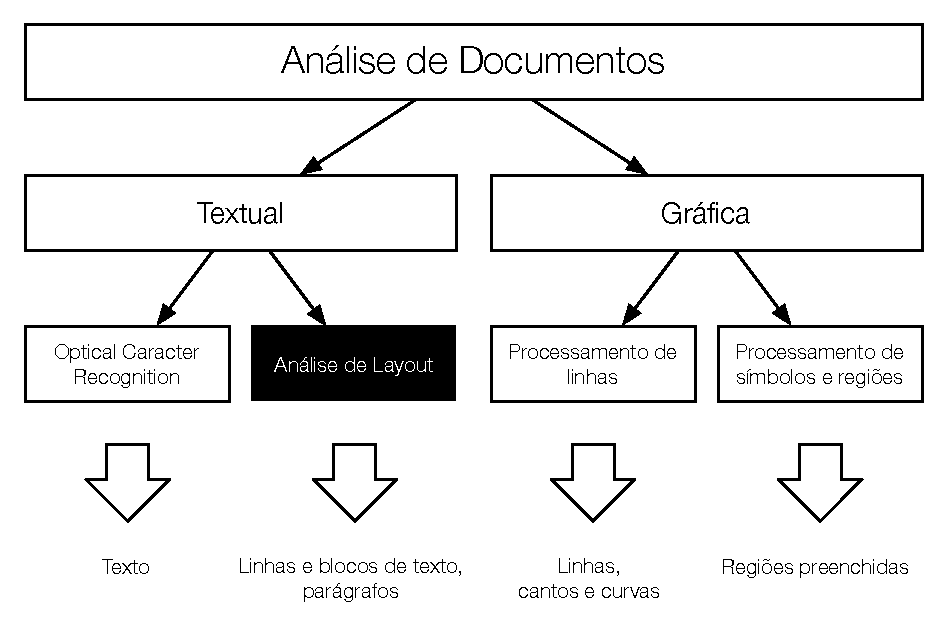
\includegraphics[width=0.7\textwidth]{assets/document_processing_areas_hierarquies.pdf}
\end{center}
\caption{Contextualização do tema do trabalho entre as áreas da
  análise de documentos. Adaptado de~\cite{Kasturi_OGorman_Govindaraju_2002}.}
\label{fig:context1}
\end{figure*}

Segmentação de página refere-se à tarefa de separar e rotular os diferentes
componentes que fazem parte da estrutura das páginas de um
documento, tais como: blocos de texto, gráficos, figuras, títulos,
legendas, separadores, tabelas, fórmulas matemáticas e regiões com
ruído.

Em geral, a segmentação de página é um dos primeiros passos no
processo de entendimento de um documento. Uma vez identificados os
blocos estruturais, processamentos específicos para cada tipo de bloco
podem ser aplicados. Por exemplo, no caso de blocos de textos é
conveniente fazer o reconhecimento de texto para que o mesmo possa ser
armazenado em formato texto (e não imagem). Por outro lado, no caso de
imagens, pode ser interessante armazená-las em alta resolução para
manter a qualidade. Documentos digitalizados podem ser processados
eficientemente em processos que envolvem armazenamento, edição,
transmissão, ou busca, por exemplo.

Devido a grande quantidade de documentos, é interessante que o seu
processamento seja realizado de forma automatizada ou pelo menos
semi-automatizada. Para tal, diversas soluções computacionais vêm
sendo propostas para o problema ao longo dos anos desde o surgimento
desse campo de pesquisa. Automatizar esta tarefa reduz custos, aumenta
a velocidade e capacidade de processamento de documentos além de
possivelmente reduzir a taxa de erro humano na classificação de uma
região.

Neste trabalho exploraremos a aplicabilidade de operadores
morfológicos automaticamente gerados ao problema de segmentação de
páginas.

Este texto está organizado da seguinte forma. Na seção~\ref{sec:fundamentos},
apresentamos as definições e conceitos básicos que serão importantes
para a leitura deste texto. Na seção \ref{sec:op_morph} explicamos com maior profundidade a principal ferramenta utilizada para realizar a segmentação: operadores morfológicos automaticamente gerados. Na seção \ref{sec:metodologia} apresentamos como utilizamos todos os conceitos para resolver o problema. Na seções \ref{sec:experimentos} e \ref{sec:resultados} detalhamos os experimentos e apresentamos os resultados. Finalmente na seção \ref{sec:conclusao} fazemos a conclusão do trabalho.

\clearpage

\section{Fundamentos}
\label{sec:fundamentos}

\subsection{Imagens digitais}
  Uma imagem digital monocromática pode ser definida como uma função $f:
  E \subset \mathbb{Z}^2 \to K = \{0,1,\ldots,k-1\}$, na qual $k$ representa o número de tons de cinza. Tipicamente adota-se $k=256$, ou seja, 8-bits de cor. Quando $k=1$ as imagens são denominadas {\bf binárias}; quando $k>1$ as imagens são denominadas {\bf tons de cinza}. Na prática, o domínio $E$ é um retângulo finito de dimensões $m\times n$ (uma matriz de $m$ linhas e $n$ colunas).

  Uma imagem RGB (colorida) é uma função $f: E \to K^3$, onde cada componente $K$ representa a intensidade das cores vermelho, verde e azul, respectivamente.

\subsection{Operadores de imagens}
Um operador de imagens é uma função que mapeia imagens em
imagens. Denotando $E=\mathbb{Z}^2$, $K=\{0,1,\ldots,k-1\}$ e
todas as imagens definidas em $E$ por $K^{E}$,
  podemos representar um operador de imagens como $\Psi: K^{E}
    \to K^{E}$.

  \subsubsection{Operadores morfológicos binário}

    Uma função $f \in \{ 0, 1 \}^E$ pode ser vista como indicadora de um conjunto $S_f \subseteq E$, ou seja, para todo $x \in E$, $x \in S_f \Leftrightarrow f(x) = 1$. Desta forma, uma função binária pode ser vista como um conjunto. Uma função entre imagens pode ser vista como uma função entre conjuntos. Conjuntos adicionados da relação de inclusão constituem algebricamente um reticulado booleano. Operadores morfológicos binários são operadores vistos como mapeamentos entre reticulados booleanos.

  \subsubsection{Operadores localmente definidos e invariantes por translação}

    Duas classes de operadores são importantes para o entendimento de operadores automaticamente gerados: localmente definidos e invariantes por translação.

    Sejam $x$ e $y$ pertencentes a $E$, $x + y$ denota a soma vetorial em $E$. Dado um conjunto $X \subseteq E$, $X_z = \{ x + z \colon x \in X \}$ denota a translação de $X$ por $z$

    Seja $W \subseteq E$, chamado de janela ou elemento estruturante, um operador $\Psi$ é dito localmente definido em relação a $W$, para todo $X \subseteq E$, se,

    \begin{equation}
      [\Psi(X)](x) = [\Psi(X \cap W_x)](x).
    \end{equation}

    Operadores localmente definidos podem ser caracterizados por funções locais \cite{Tomita:1996:PrAuMa}. Ou seja, independentemente to tamanho do conjunto $X$, $\Psi(X)$ pode ser visto como uma função booleana $\psi_x \colon \{0, 1\}^n \rightarrow \{0, 1\}$, onde $n = |W|$, da seguinte forma:

    \begin{equation}
      [\Psi(X)](x) = \psi_x(X_{-x} \cap W),
    \end{equation}

    onde $X_{-x} \cap W$ denota a atribuição de valores de $x \in X$ às variáveis $x_i$ da função booleana, de acordo com a regra $x_i = 1 \Leftrightarrow w_i \in X_{-z} \cap W$, ou equivalentemente, se $w_i + z \in X$.

    Se $\Psi$ também for invariante por translação então teremos $\psi_x = \psi_y$ para $x, y \in E$. Operadores localmente definidos e invariantes por translação são chamados de W-operadores, operadores de janela.

    Alguns exemplos de operadores desta classe são dilatação \eqref{eq:dilatacao} e erosão \eqref{eq:erosao}, ditos operadores elementares.

    \begin{equation}
      \label{eq:dilatacao}
      \delta_{B}(X) = \{ x \in E \colon B_{x} \cap X \neq \emptyset \}
    \end{equation}

    \begin{equation}
      \label{eq:erosao}
      \varepsilon_{B}(X) = \{ x \in E \colon B_{x} \subseteq E \}
    \end{equation}

\subsection{Classificação de objetos}

Na área de reconhecimento de padrões e aprendizado computacional
estudam-se métodos e técnicas para classificação de dados em geral. Os
dados (padrões) a serem classificados correspondem, em geral, à
representação digital de algum objeto concreto ou abstrato. O objetivo
da classificação é atribuir um rótulo de classe a cada padrão
observado.

Dependendo do problema, os rótulos de classe podem ser conhecidos ou
não. Por exemplo, se desejamos fazer o reconhecimento de caracteres,
os padrões são a imagem dos caracteres e os rótulos de classe são as
identificações dos possíveis caracteres. Por outro lado, em problemas
como na classificação de perfil de consumidores, pode não haver um
conjunto de perfis pré-estabelecidos e o objetivo seria então
identificar a possível existência de perfis. O primeiro é conhecido
como problema de classificação supervisionada e o segundo como
classificação não-supervisionada.

No caso da classificação supervisionada, supõe-se que os padrões são
elementos de um espaço $X$ e que o conjunto de rótulo de classe é dado
por $Y=\{y_1,y_2,\ldots,y_c\}$. Assim, um classificador pode ser
expresso por uma função $f: X \to Y$.

Frequentemente $X$ é um subespaço de $\mathbb{R}^d$. Assim, um padrão
é representado por uma $d$-upla $\mathbf{x}=(x_1,x_2,\ldots,x_d) \in
\mathbb{R}^d$.

\subsection{Segmentação de imagens}

A segmentação de imagens é um processamento comum a praticamente
todos os processos que envolvem análise de imagens. Segmentar uma
imagem corresponde a particionar o seu domínio, de forma que cada
região resultante corresponda (do ponto de vista semântico) a uma
componente de interesse na análise em questão. Este problema pode ser modelado como uma classificação de objetos, onde o conjunto de pixeis de uma imagem são os objetos em $X$ e as componentes em $Y$ são regiões de interesse.

\subsection{Classificação dos componentes}
\label{sec:components}

O problema de segmentação de imagens de documentos pode ser modelado como um problema de classificação de objetos, onde cada pixel da imagem é rotulado através de uma função classificadora

\begin{equation}
\Psi \colon \mathbb{E} \rightarrow \mathbb{Y}
\end{equation}

sendo $\mathbb{Y}$ um conjunto composto pelas regiões de interesse:

\begin{itemize}
  \item blocos de texto: região com parágrafos
  \item gráficos
  \item figuras
  \item títulos
  \item legendas
  \item separadores
  \item tabelas
  \item fórmulas matemáticas
  \item regiões com ruído
\end{itemize}

Neste trabalho utilizaremos operadores morfológicos binários como classificadores de imagens. O processo todo será descrito na seção \ref{sec:metodologia}.

\clearpage

\section{Operadores morfológicos automaticamente gerados}
\label{sec:op_morph}

Construir operadores morfológicos que resolvam problemas complexos como o de segmentar uma página de documento, pode ser uma tarefa que demande muito tempo, experiência e conhecimento específico do assunto. Como estas imagens possuem características distintas dependendo da publicação (diferentes jornais e revistas), é possível que apenas um operador não consiga ser aplicado a todas as imagens. Ou seja, construir operadores com facilidade é um fator sensível para a viabilização desta abordagem.

Nesta seção apresentamos um método para projetar operadores morfológicos de forma automática utilizando técnicas de aprendizado computacional.

O método proposto na tese de mestrado de Nina S. T. Hirata \cite{Tomita:1996:PrAuMa} requer que um conjunto de pares de imagens sejam fornecidos para uma etapa inicial de treinamento. Estes pares contém uma imagem {\bf original} e sua {\bf ideal}, ou seja, a mesma imagem porém modificada como desejamos que o método aprenda a reproduzir em outras imagens.

A partir deste conjunto de treinamento um operador é gerado, o qual podemos aplicar a outras imagens.

\subsection{Formalização}

Assumimos que as imagens originais e ideias são realizações dos conjuntos aleatórios $S$ e $I$, com distribuição de probabilidade conjunta $P(S,I)$. Supõe-se que esta função seja caracterizada por um processo local $(S \cap Wz, I(z))$, com $S \cap Wz \in P(W_z)$, conjunto potência de $W_z$, e $I(z) \in \{0, 1\}$. Ou seja, as imagens de exemplo passam a ser vistas como realizações de conjuntos aleatórios localmente definidos pela janela $W$. Denotaremos este processo por $(X, y)$.

Desta forma, o trabalho de construção de um operador l.d. e i.t. $\psi$ que se aproxime do operador ideal $\Psi$, passa a ser o de minizar o erro absoluto médio ($MAE$), dado pela seguinte expressão:

\begin{equation}
  MAE(\Psi) = E[|\psi(X) - y|].
\end{equation}

Desenvolvendo a expressão acima, chegamos ao critério para decidir o valor de $\psi(X)$ para cada $X$.

\begin{equation}
\begin{array}{rcl} 
  MAE(\Psi) & =  & \sum\limits_{(X, y)} |\psi(X) - y | P(X,y) \\
  & =  & \sum\limits_{(X, 0)} \psi(X)P(X, 0) + \sum\limits_{(X, 1)} |\psi(X) - 1|P(X, 1) \\
  & = & \sum\limits_{X \colon \psi(X) = 1} P(X, 0) + \sum\limits_{X \colon \psi(X) = 0} P(X, 1)
\end{array}
\end{equation}

Ou seja, para minimizar o $MAE$ basta que escolhamos de forma adequada os valores de $\psi(X)$ de acordo com estimativas das probabilidades $P(X,0)$ e $P(X, 1)$ através da observação dos exemplos fornecidos.

A seguir detalhamos as etapas envolvidas na construção de $\psi$.

\subsection{Coleta}

Seja $C(X_W) = \{X \cap W + z \colon z \in E \}$ o conjunto de todas as configurações observadas ao se transladar a janela $W$ sobre a imagem $X$. Seja $Y_z$ o valor 0 ou 1 encontrado na imagem $Y$ na posição $z$. Construímos uma tabela com três colunas: $C(X_W)$, frequência observada $Y_z = 0$ e frequência $Y_z = 1$.

O resultado desta etapa é uma estimativa $\hat{P}(X, y)$ de $P(X, y)$.

\subsection{Decisão}

As configurações observadas na etapa anterior possuirão valores relacionados em $Y$ iguais a 0, 1 ou ambos. No caso de tanto 1 como 0 terem sido observados, escolheremos como valor para a função final a com maior número de ocorrências. No caso de alguma configuração não ter sido observada ou de o número de ocorrências empatar, escolheremos o valor que simplifica a próxima etapa: minimização.

Formalmente, se $\hat{P}(X, 1) > \hat{P}(X, 0)$, então $\psi(X) = 1$, do contrário $\psi(X) = 0$.

\subsection{Minimização}

Na etapa anterior é usual que nem todos os padrões possíveis para $X$ sejam observados. Logo precisamos completar a definição da função $\psi(X)$. Para tanto utilizamos um minimizador de funções booleanas chamado ISI. Ele não só completa a função como também produz uma representação mais compacta utilizando intervalos maximais.

Um algoritmo bastante conhecido para realizar a minimização de funções booleanas é o algoritmo de QM (Quine-McCluskey), onde através de combinações dois a dois dos mintermos de uma expressão booleana procura-se criar cubos cada vez maiores, eliminando depois os cubos sobressalentes a fim de obter uma cobertura mínima da função.

Porém esta etapa de combinação dois a dois tende a ser computacionalmente ineficiente. Além de que a etapa para identificação dos n-cubos primos (aqueles que não podem ser descartados) é muito custosa computacionalmente.

Por estes motivos, a biblioteca TRIOS \cite{dostrios}, que implementa todo o processo descrito nesta seção, utiliza um outro algoritmo denominado ISI. Este algoritmo inicia com o n-cubo, representado na forma do intervalo $[\emptyset, W]$ e a cada iteração remove um ponto do n-cubo equivalente um mintermo negativo. Desta forma quebrando o intervalo inicial em outros $N$ intervalos. Após eliminar todos os mintermos negativos chegamos um conjunto de intervalos maximais que representam a função. Uma descrição mais detalhada do algoritmo pode ser encontrada em \cite{Tomita:1996:PrAuMa}.

Esta é a última etapa do processo. Podemos agora aplicar o operador a outras imagens.

\clearpage

\section{Metodologia}
\label{sec:metodologia}

O método proposto é baseado em operadores morfológicos automaticamente gerados, ou seja, construímos um segmentador genérico a partir de alguns exemplos de segmentação (pares de imagens). A seguir detalhamos cada uma das etapas envolvidas.

    \begin{enumerate}
      \item Preparação das imagens de treinamento
      \item Construção dos operadores
      \item Aplicação dos operadores
      \item Consensualização
    \end{enumerate}

    \subsection{Preparação das imagens de treinamento}

      O primeiro passo consiste na produção dos pares de imagens de treinamento. Estes pares consistem da imagem original binarizada e de sua variante segmentada.

      Para cada imagem original geramos $n$ pares de exemplo, sendo $n$ o número de tipos de regiões que desejamos segmentar. No caso deste trabalho nos limitamos a dois: textos de parágrafos e título.

      A variante segmentada consiste da imagem original com a região de interesse apagada (em braco). A tabela \ref{tab:imgset_example} é um exemplo com uma imagem original, binarizada e suas variantes.

      \begin{table}[hbt]
        \caption{Exemplo de preparação de imagem para treinamento do operador}
        \begin{center}
          \begin{tabular}{c c c c}
            Original & Preto e branco & Exemplo de parágrafo & Exemplo de título \\
            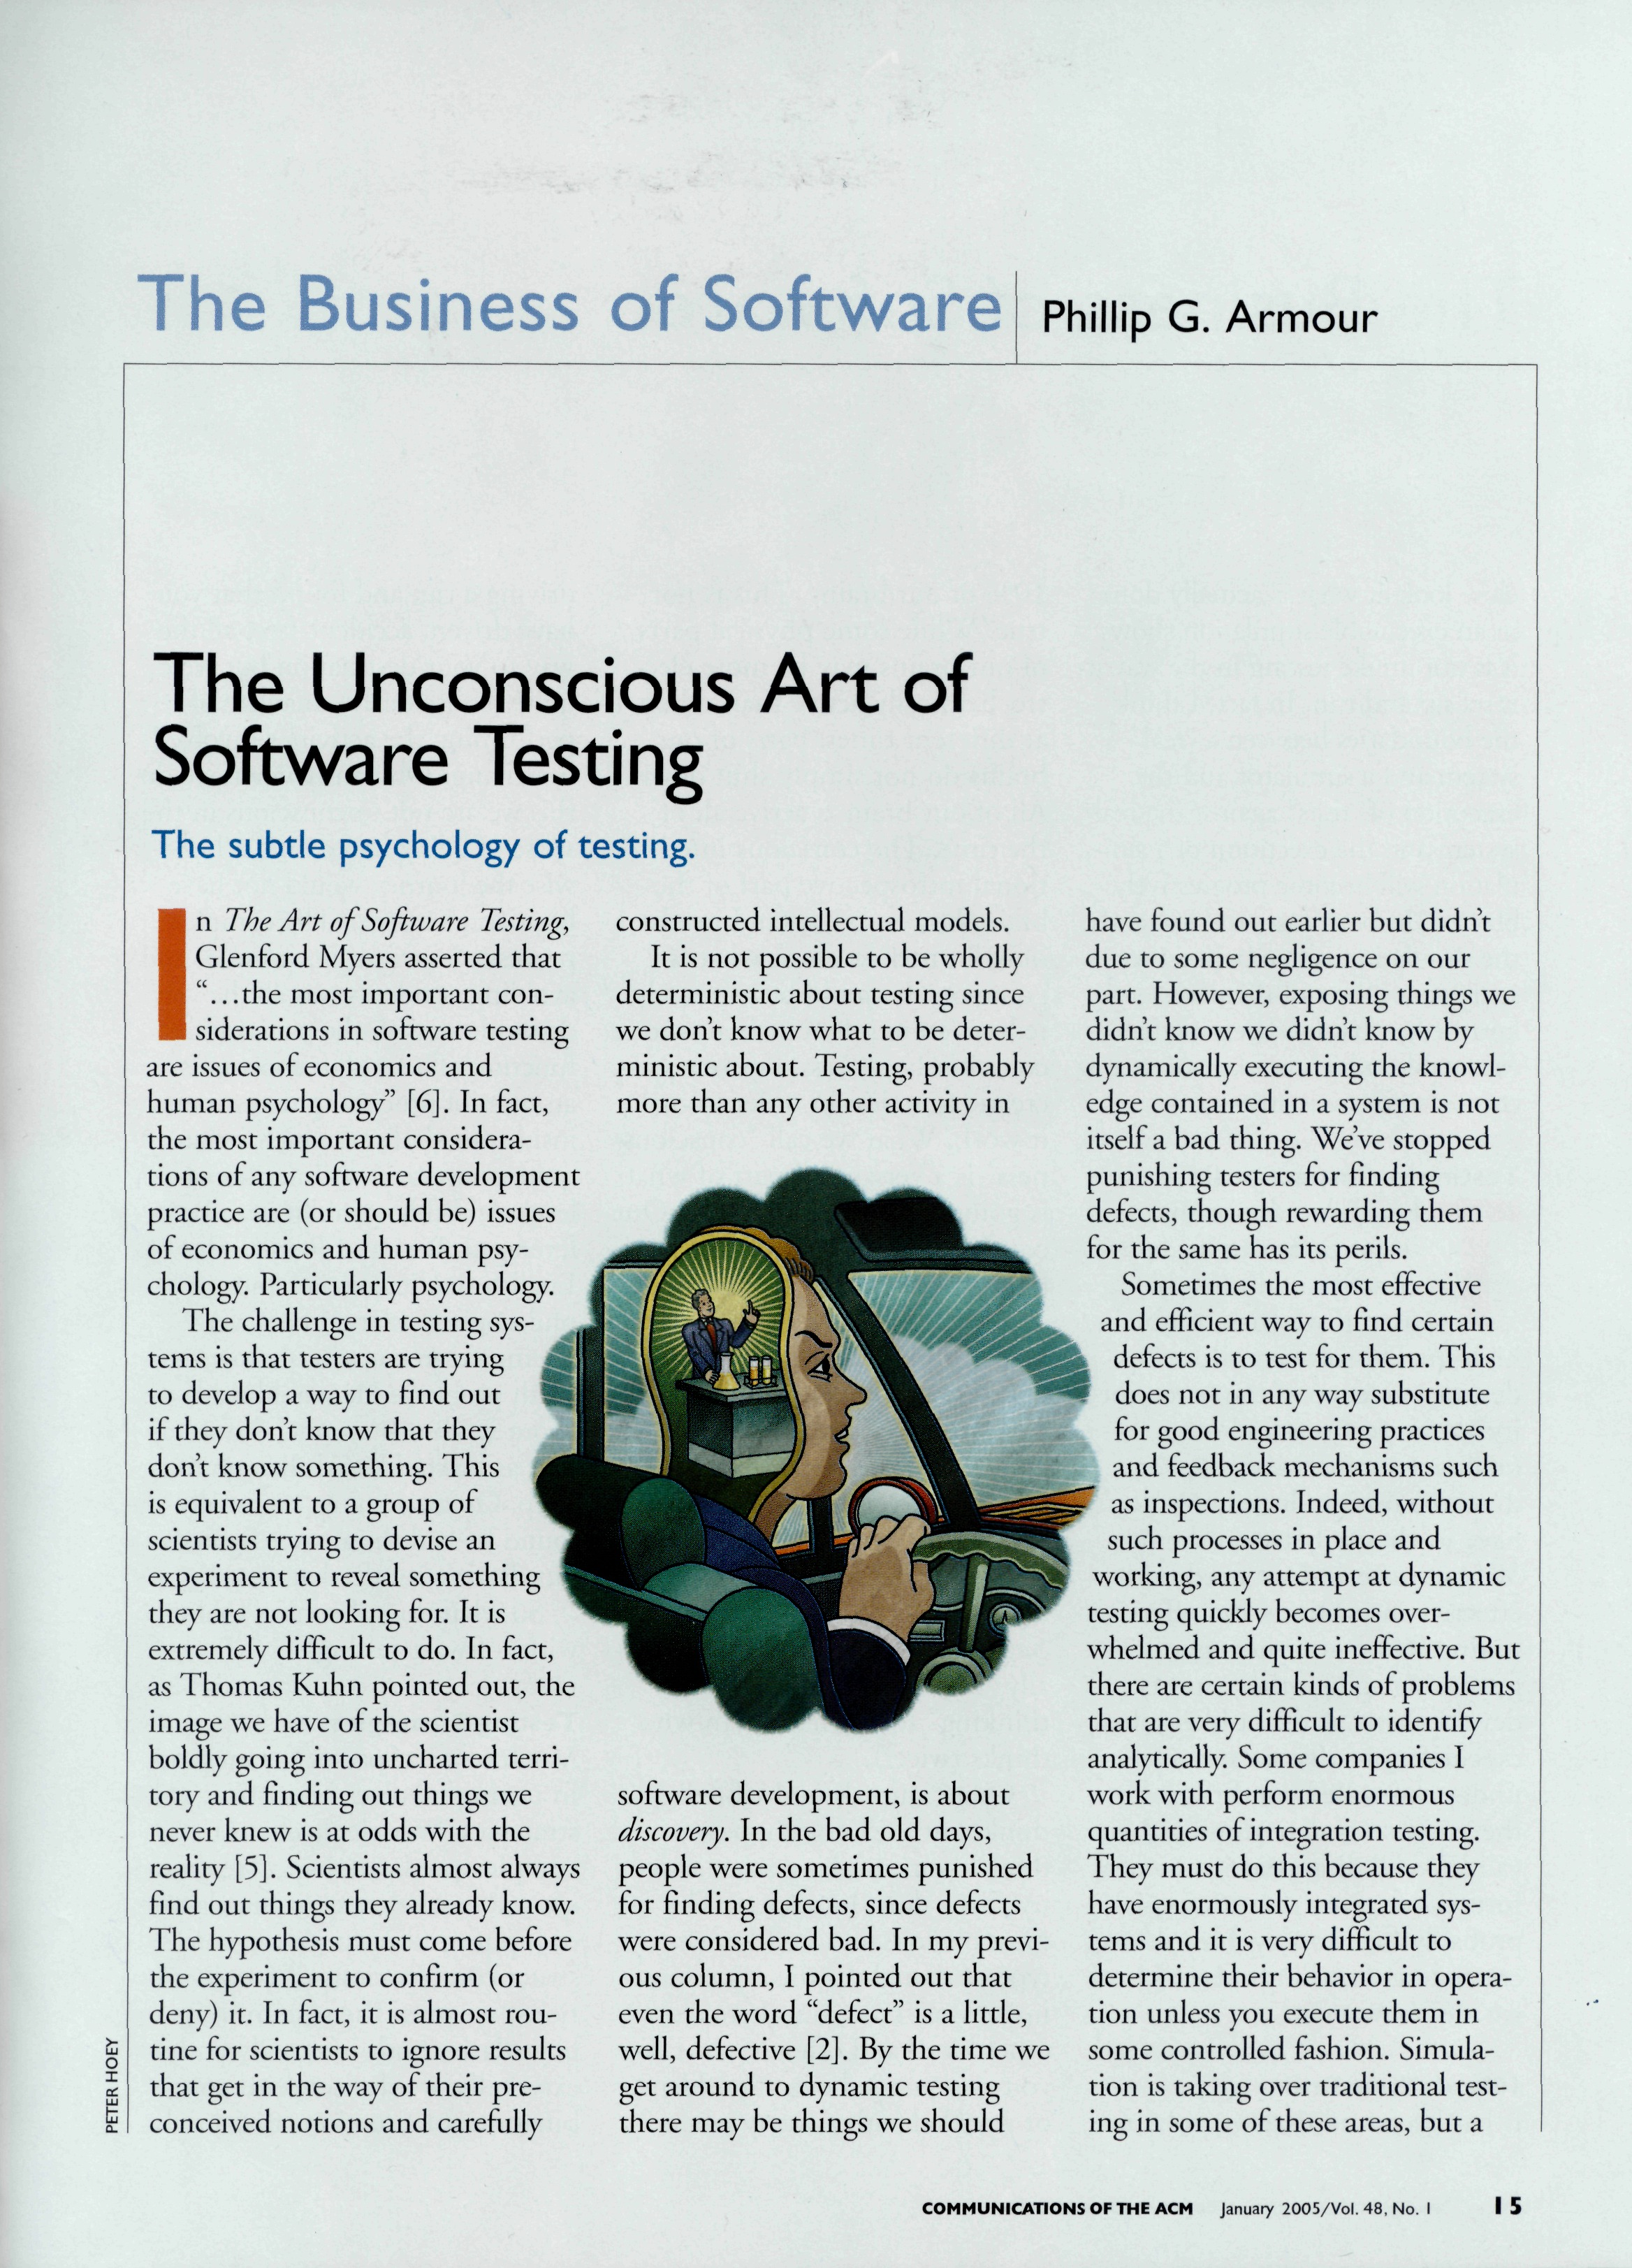
\includegraphics[width=0.2\textwidth]{assets/00000802.png}
            &
            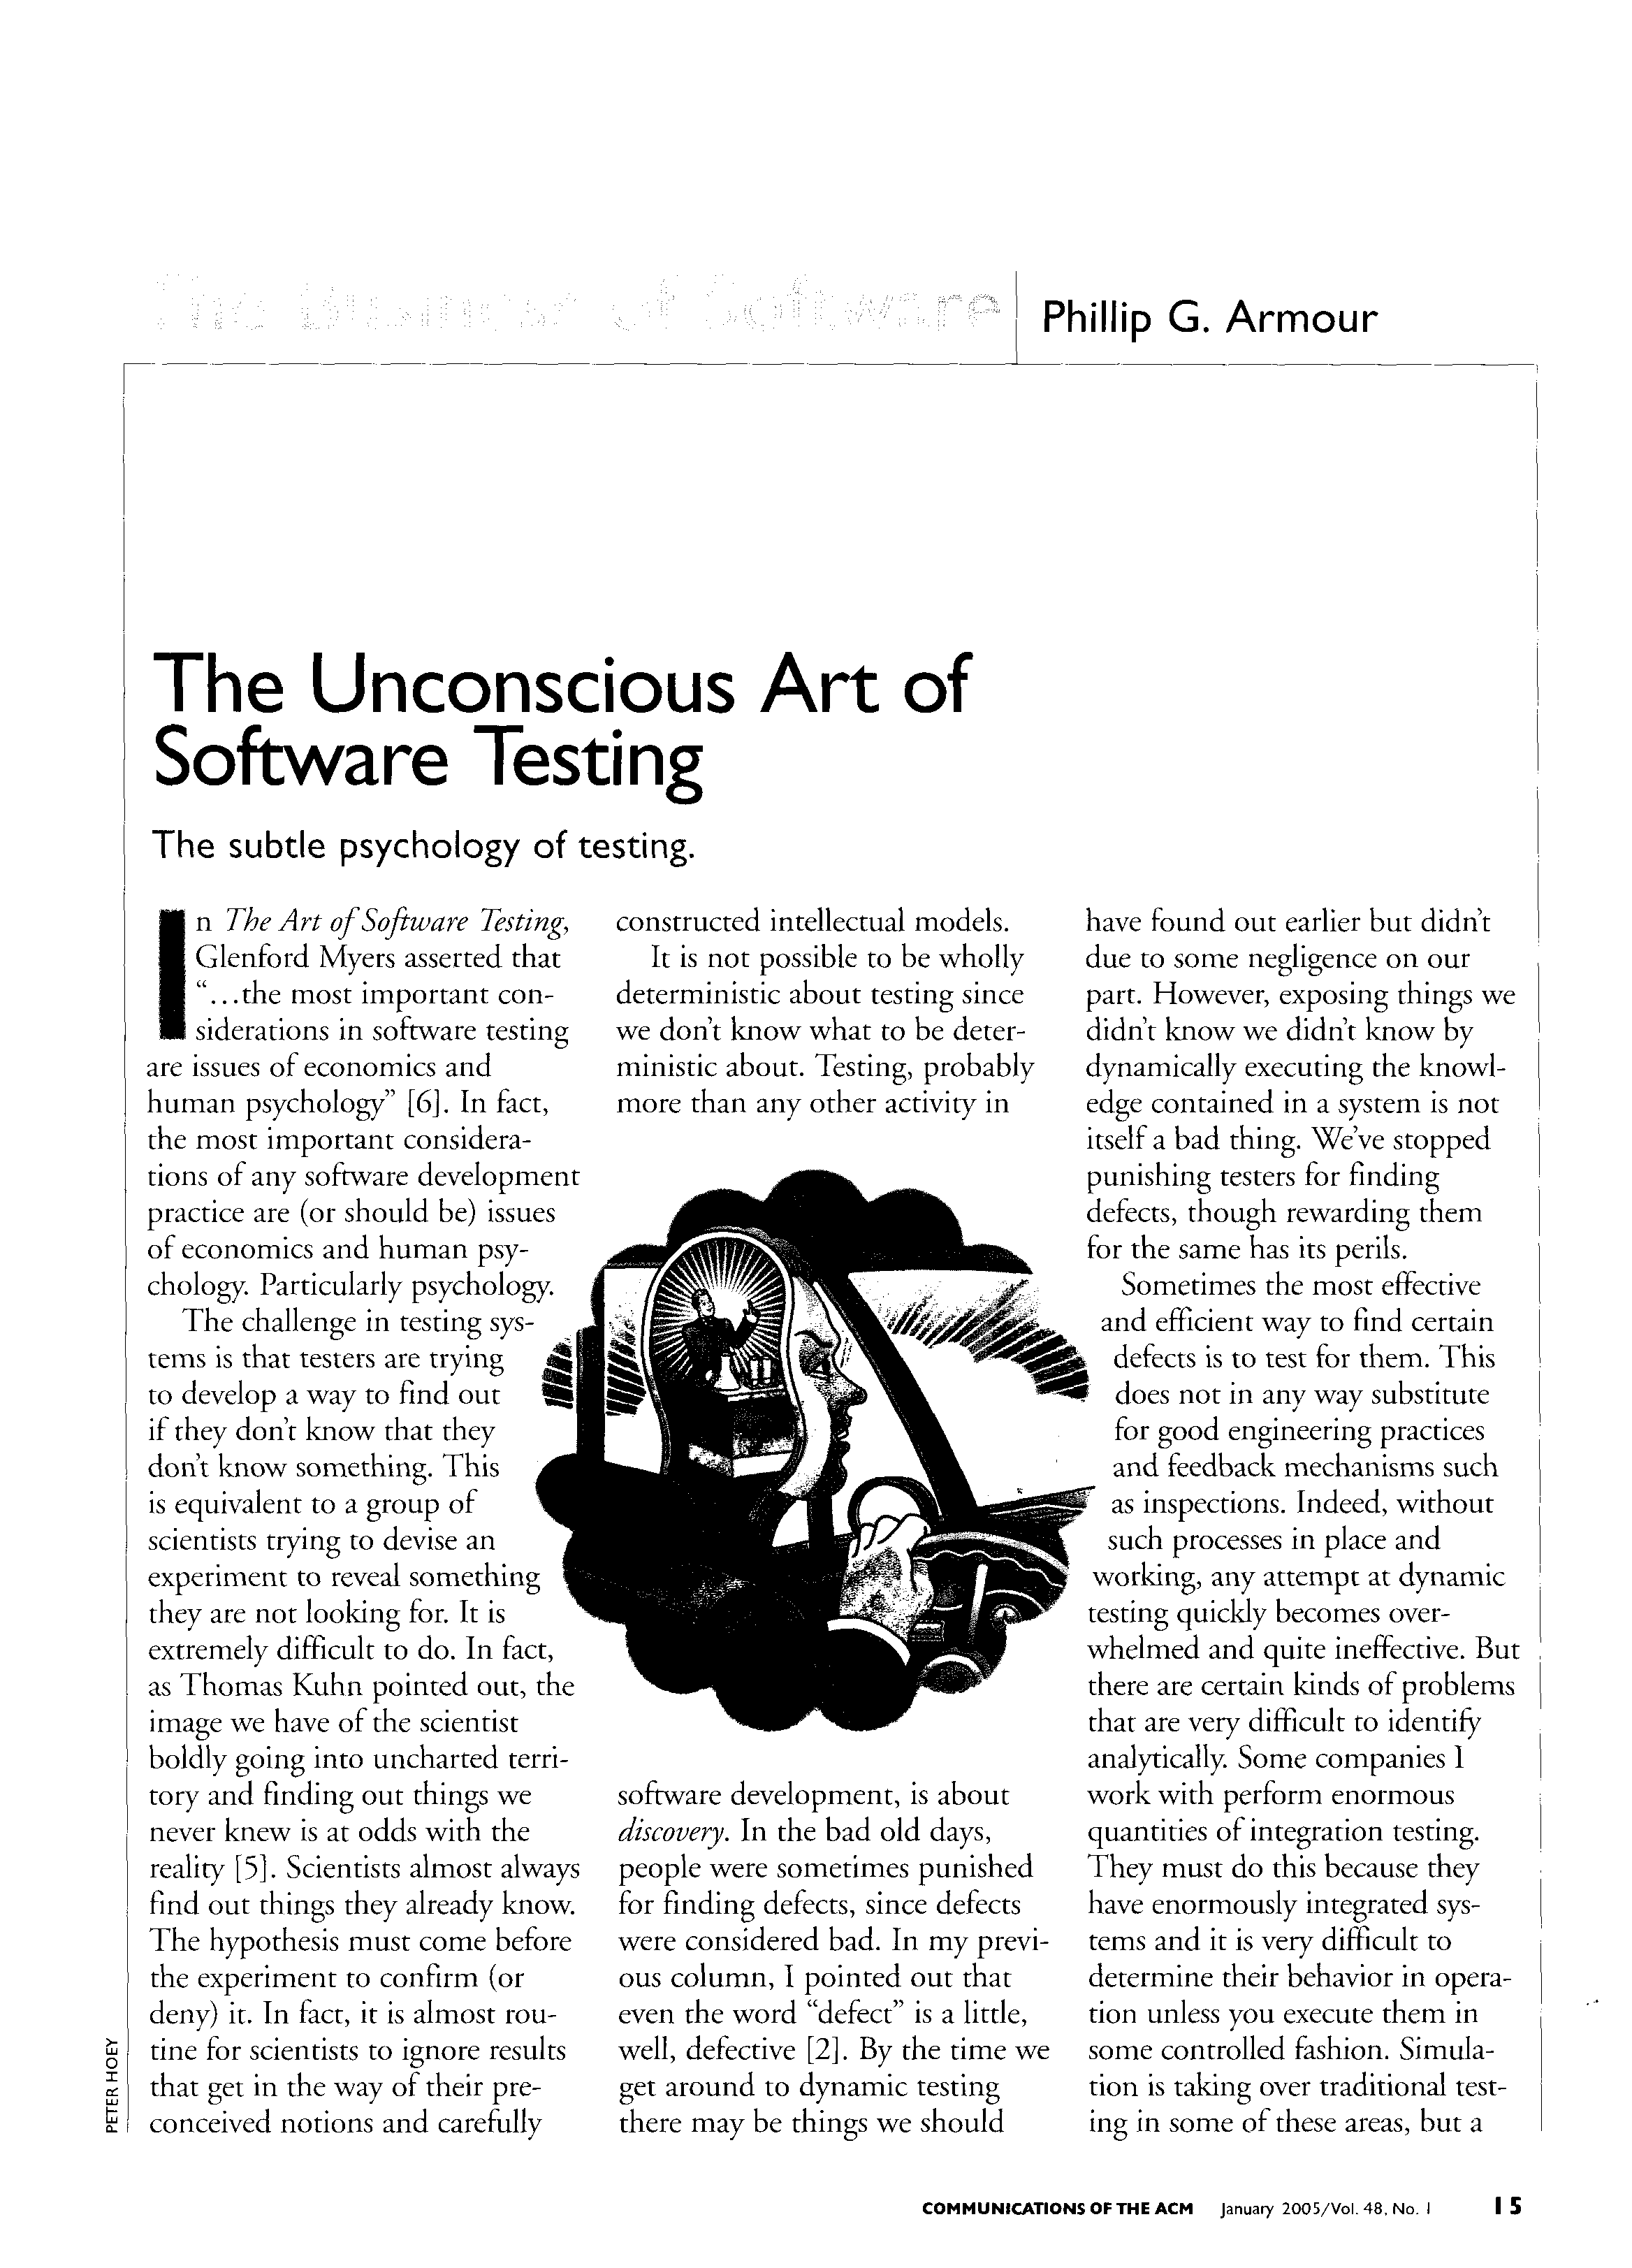
\includegraphics[width=0.2\textwidth]{assets/original_images/cacm/802_black_and_white.png}
            &
            
\includegraphics[width=0.2\textwidth]{assets/802_TextRegion_paragraph.png}
            &
            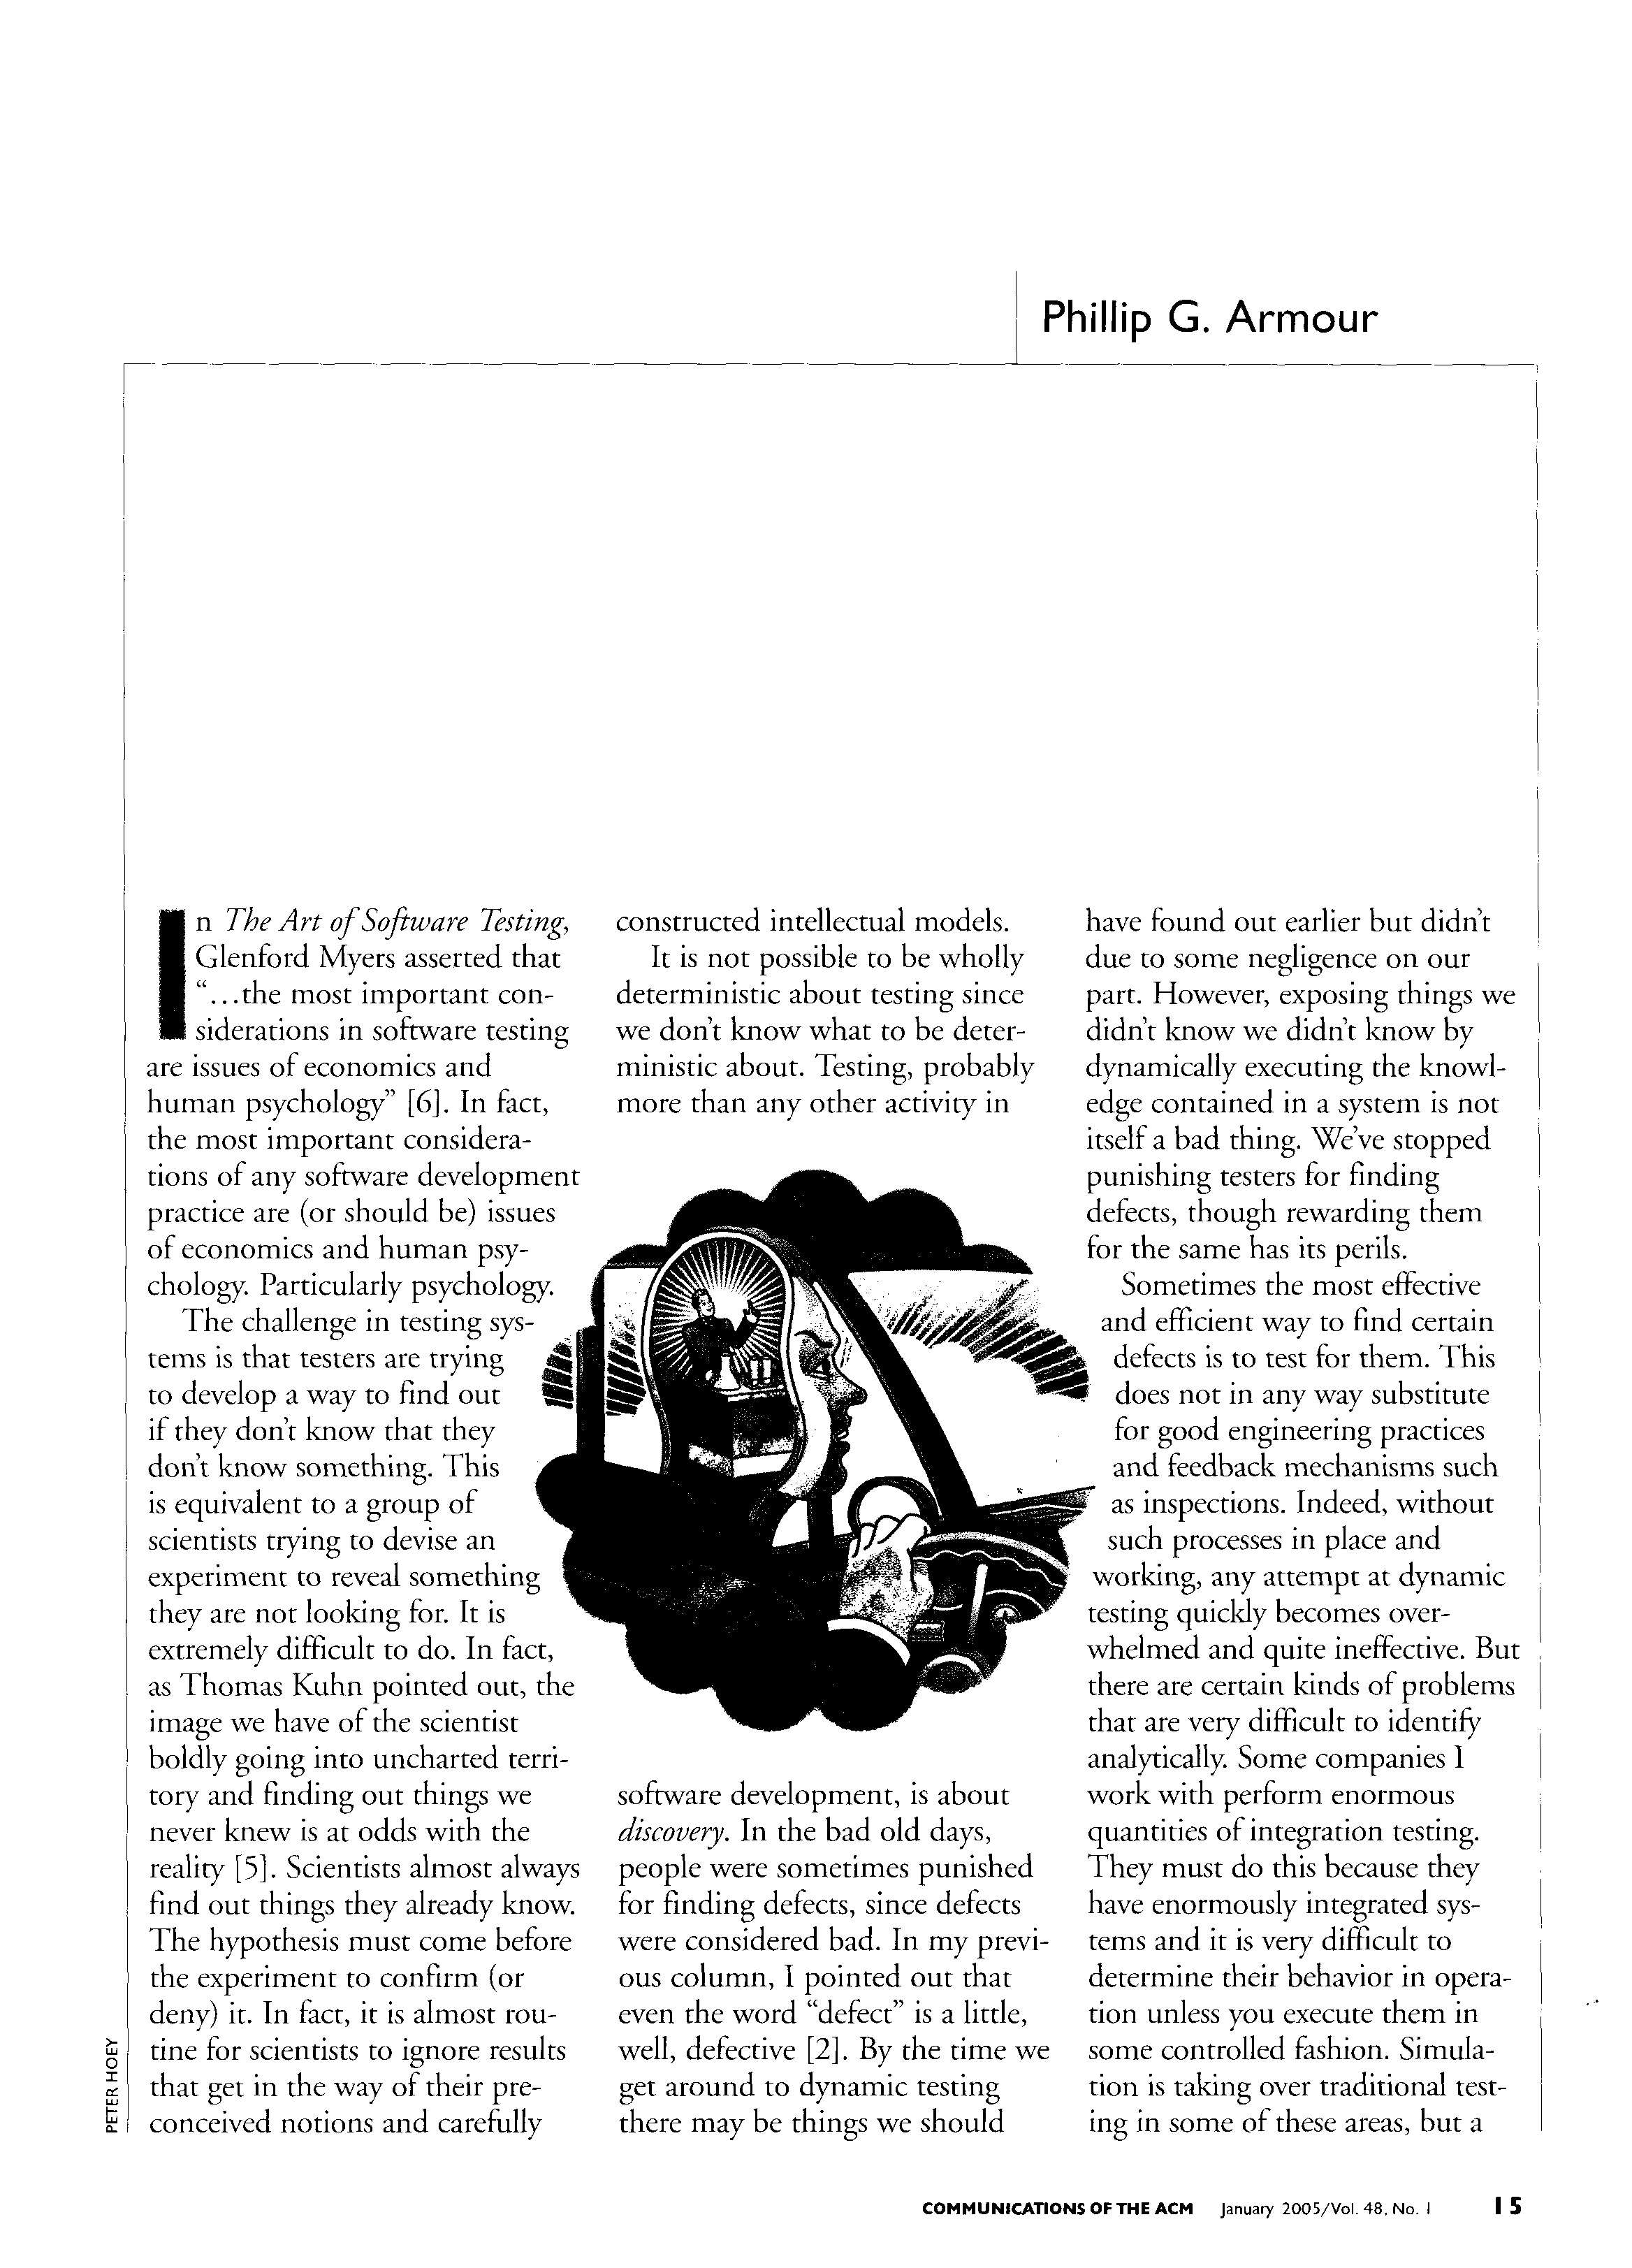
\includegraphics[width=0.2\textwidth]{assets/802_TextRegion_heading.png}
          \end{tabular}
        \end{center}
        \label{tab:imgset_example}
      \end{table}

      O processo de binarização foi melhor detalhado no apêndice \ref{sec:otsu}.

    \subsection{Construção dos operadores}

      O algoritmo gerador de operadores morfológicos recebe como entrada um conjunto de pares de imagens de exemplo do passo anterior. Treinamos um operador para cada tipo de região utilizando a biblioteca TRIOS \cite{dostrios}. Os parâmetros para o treinamento foram ajustados experimentalmente como apresentado na seção \ref{sec:experimentos}.

    \subsection{Aplicação dos operadores}

      Construídos os operadores para cada tipo de região, aplicamos todos os operadores às imagens que desejamos segmentar obtendo um resultado para cada operador. Sendo $n$ operadores e $m$ imagens, obtemos $nm$ resultados. A tabela \ref{tab:aplicacao} demonstra a aplicação dos operadores de parágrafo e título a uma imagem.

      \begin{table}[hbt]
        \caption{Exemplo de preparação de imagem para treinamento do operador}
        \begin{center}
          \begin{tabular}{c c c}
            Original & Operador de parágrafo & Operador de título \\
            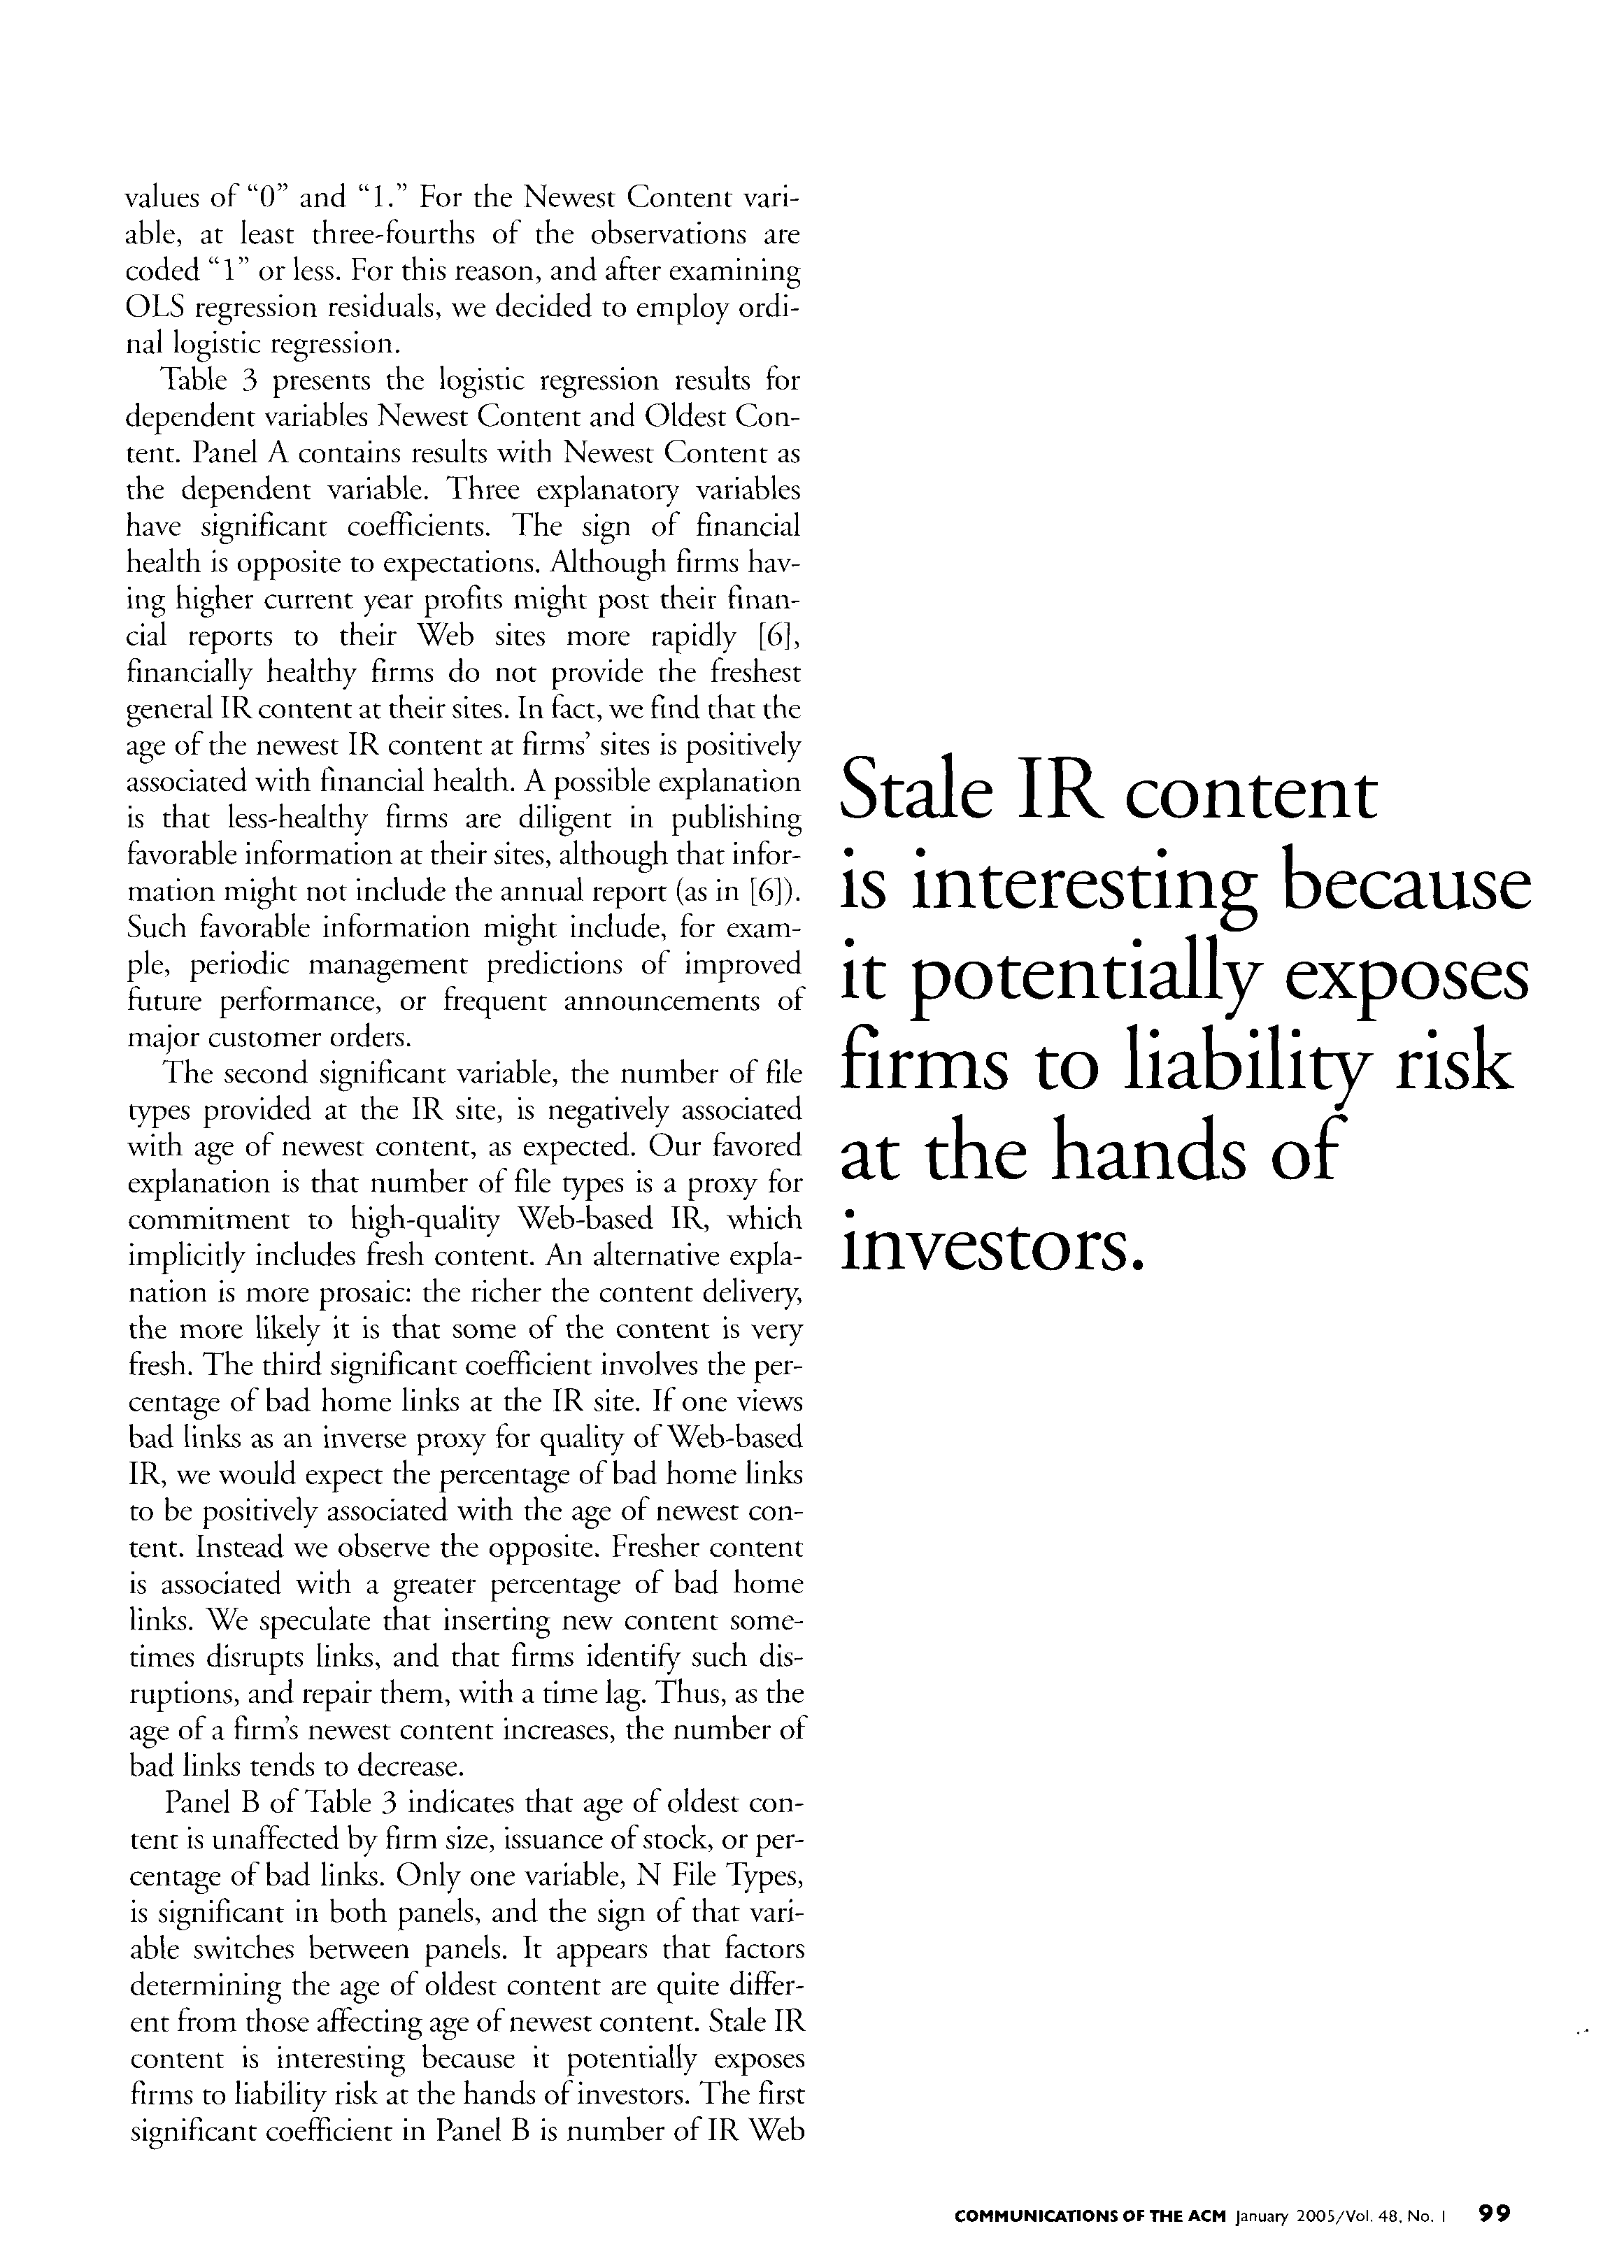
\includegraphics[width=0.2\textwidth]{assets/exemplo_aplicacao/695_black_and_white.png}
            &
            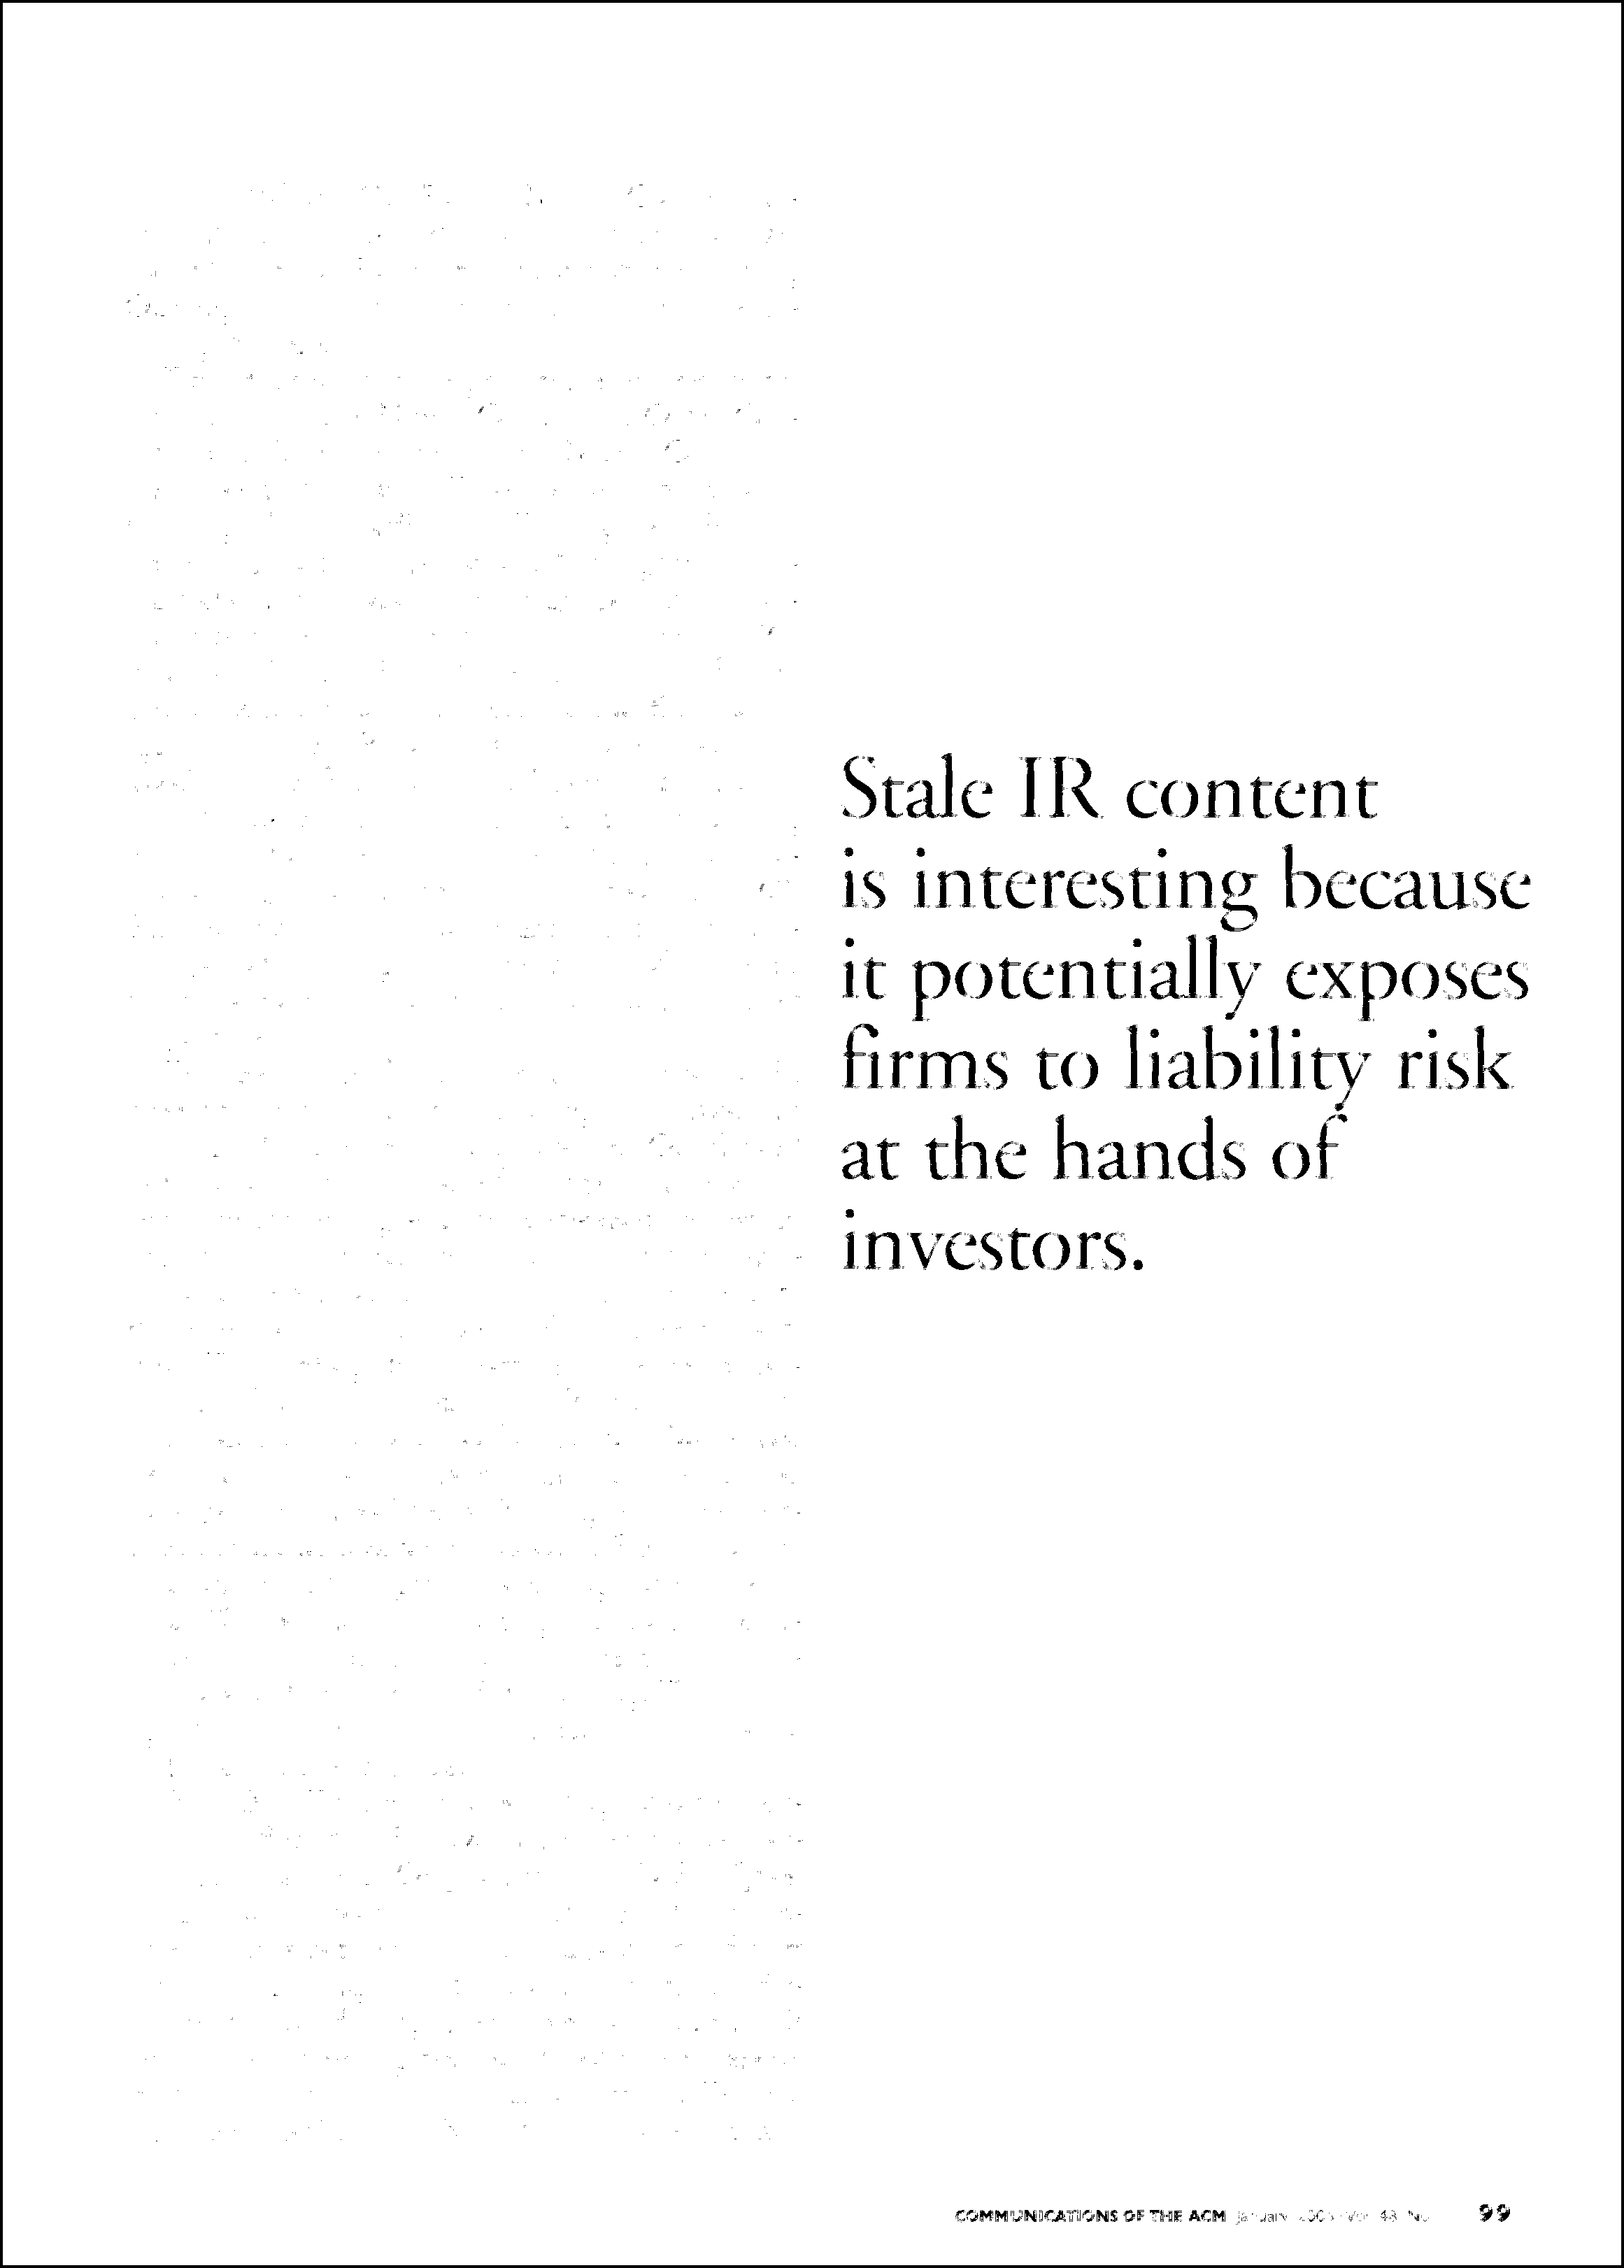
\includegraphics[width=0.2\textwidth]{assets/exemplo_aplicacao/695_paragraph.png}
            &
            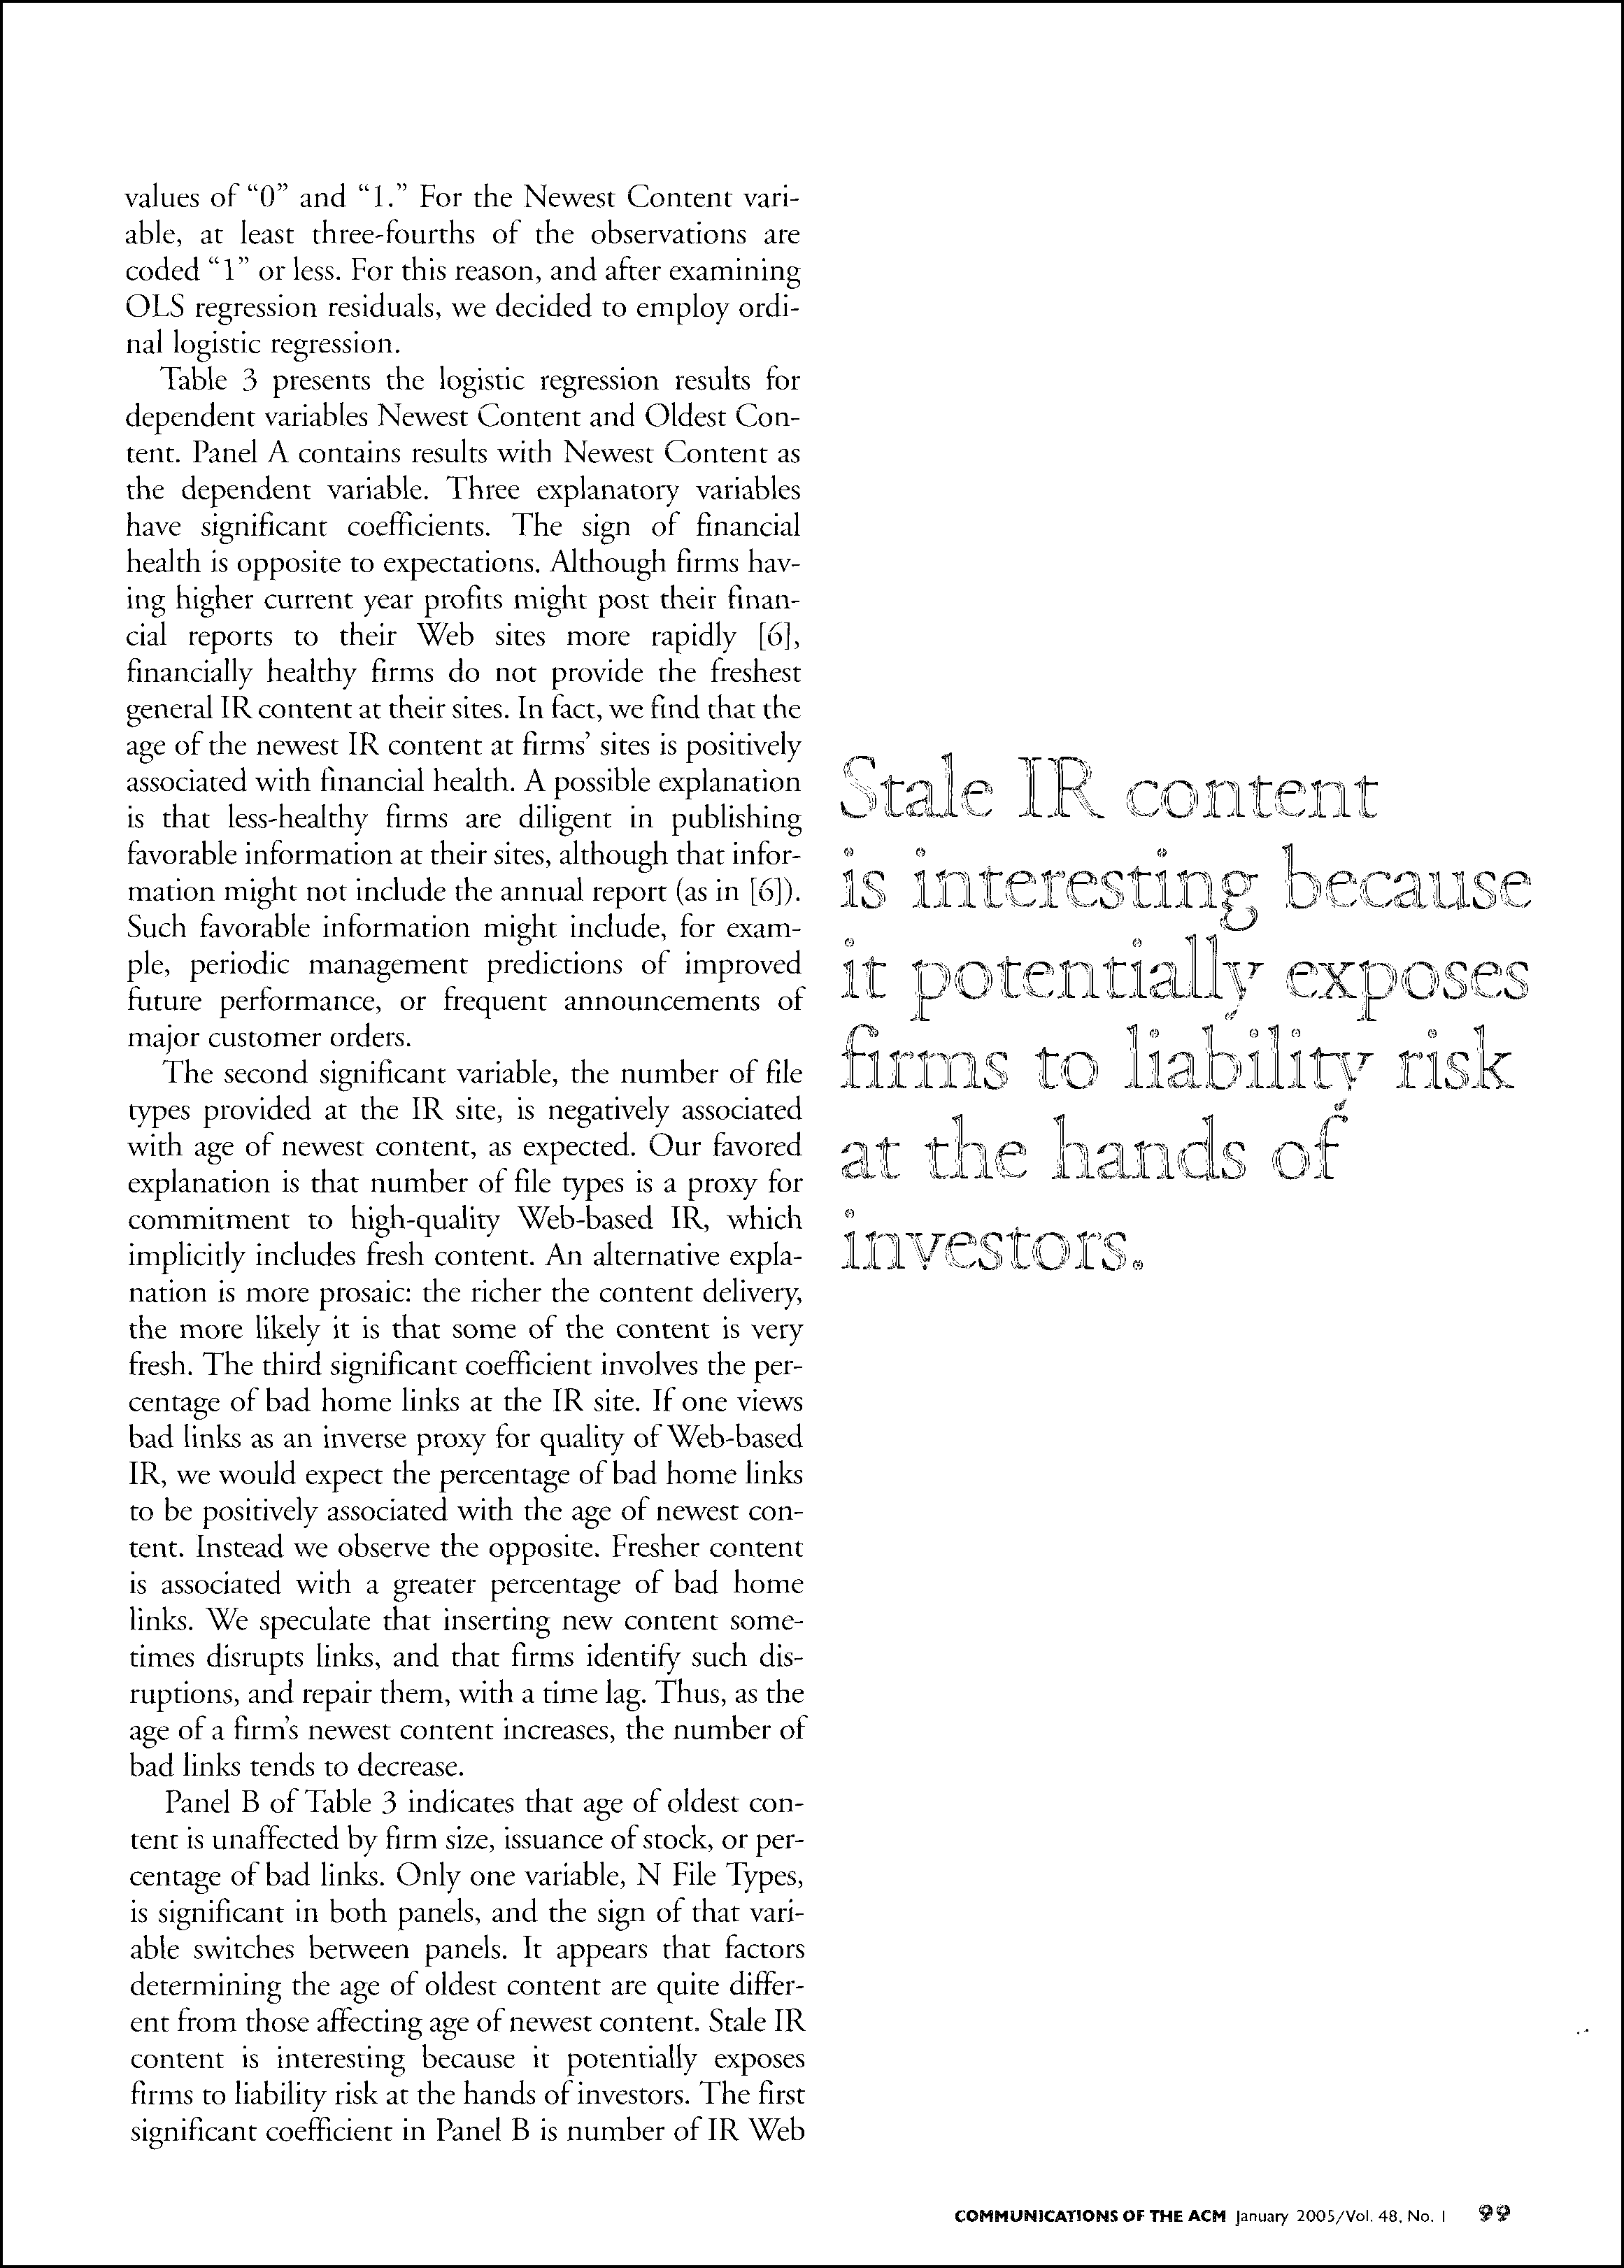
\includegraphics[width=0.2\textwidth]{assets/exemplo_aplicacao/695_heading.png}
          \end{tabular}
        \end{center}
        \label{tab:aplicacao}
      \end{table}

    \subsection{Consensualização}

      A aplicação de operadores diferentes à mesma imagem pode gerar resultados incoerentes. Pixeis classificados como pertencentes a mais de uma região fazem com que a união dos resultados seja impossível sem nenhum tipo de processamento. Para concluirmos a segmentação é necessário chegar a um consenso sobre qual operador possui a maior probabilidade de estar certo a cada pixel de classificação conflitante.

      Partindo da observação de que pixel pertencente a uma certa região costuma estar cercados por pixeis da mesma região, aplicamos um processo de escolha por maior contagem de pixeis na vizinhança. Ou seja, se houver um conflito de classificação de um pixel entre texto ou título, conta-se quantos pixeis na vizinhança pertencem a uma dada região e a que obtiver maior contagem ganha.

\clearpage

\section{Experimentos}
\label{sec:experimentos}

  Realizamos experimentos variando diversos parâmetros em diferentes etapas da segmentação. Apesar de usarmos uma técnica de aprendizado computacional para automatizar parte do processo, identificar quais parâmetros produzem o melhor resultado a um custo desejável (tempo de processamento e poder computacional) é uma tarefa ainda experimental.

  A qualidade da solução e o tempo levado para processá-lo foram medidos a fim de identificar o lucus optimus, ou seja, a combinação que produz um bom resultado com um tempo de processamento razoável.

  Os parâmetros escolhidos para análise foram:

  \begin{itemize}
    \item Mistura de publicações no conjunto de treinamento.
    \item Quantidade de imagens no conjunto de treinamento.
    \item Tipos de regiões.
    \item Formatos de janelas.
    \item Tamanhos de janelas para consensualização.
  \end{itemize}

  A seguir detalhamos os valores dos parâmetros e os motivos de sua escolha.

  \subsection{Base de dados}

    As imagens utilizadas nos experimentos foram obtidas de um banco de dados construído pelos pesquisadores do PRImA ao longo de anos \cite{Antonacopoulos09arealistic}. Ele inclui um conjunto de documentos que busca simular um cenário realístico de aplicação, com layouts complexos e diferentes tipos de fontes e formatos de regiões. Isto é importante para avaliar a aplicabilidade do método em situações práticas, onde um controle sobre o formato do conteúdo seria indesejável ou inviável.

    No artigo \cite{Antonacopoulos09arealistic}, os autores apresentam um conjunto de dados com páginas de revistas, artigos científicos diversos, documentos modernos e não apenas históricos.

    O conjunto de dados contém não só imagens mas também arquivos XML \cite{pletschacher2010page} com metadados como informações bibliográficas (título, autor, publicação), informações das imagens (resolução, bit depth, modelo do scanner), características do layout (número de colunas, variedade de tamanhos de fontes) e informações administrativas (direitos autorais).

    Os documentos são digitalizados com um cartão escuro por trás para minimizar a exposição da contra página. Posteriormente um algoritmo analisa possíveis falhas, como rotação do documento, marcando-os para redigitalização. Uma correção automática não é utilizada, pois isto pode comprometer a qualidade da imagem.

    Uma vez que a imagem foi aceita no banco de dados, inicia-se um processo manual de marcação do grownd-truth. Este trabalho deve ser realizado da forma mais precisa possível, pois é a base para determinar a corretude dos algoritmos segmentadores. Por se tratar de uma etapa muito custosa, uma ferramenta semi-automática chamada Aletheia \cite{clausner2011aletheia} é utilizada para agilizar o processo. Esta ferramenta permite a uma pessoa desenhar uma região poligonal em torno de uma região de interesse. Em seguida esta região é automaticamente ajustada pelo software, como se a pessoa estivesse colocando um elástico que aperta a região.

  \subsection{Mistura de publicações no conjunto de treinamento}

    Diferentes publicações trabalham com fontes e grafismos próprios. A diferença fica evidente ao comparar um jornal antigo com uma revista sobre tecnologia. Incluir imagens de publicações diversas no mesmo conjunto de imagens de treinamento pode produzir operadores menos precisos. Mesmo entre publicações do mesmo período, podemos ter diferentes tamanhos de fontes e famílias de tipos. Este experimento tem por objetivo analisar o impacto na qualidade por tentar criar operadores mais genéricos.

    Testamos os seguintes conjuntos de imagens de treinamento:

    \begin{itemize}
      \item Comunications of the ACM: 263, 674, 677, 680, 683, 685, 686, 689, 692, 695, 802 e 803. Este conjunto é chamado de CACM neste texto.
      \item TIME Magazine: 232, 720, 721, 723, 782, 783, 784, 785 e 786. Este conjunto é chamado de TIME neste texto.
    \end{itemize}

  \subsection{Tipos de regiões}

    Os gabaritos do conjunto de dados utilizados nestes experimentos rotulam com detalhes cada região das imagens:

    \begin{enumerate}
      \item Text
      \begin{enumerate}
        \item Header 
        \item Headings (título)
        \item Capital (letras maiores)
        \item Drop Capital
        \item Credit
        \item Paragraph (parágrafo)
        \item Floating
        \item Page number
        \item Footer
      \end{enumerate}
      \item Graphic
      \item Math
      \item Chart
      \item Image
      \item Noise
      \item Separator
      \item Table
    \end{enumerate}

    Nos experimentos realizados nos limitamos a Text Heading e Text Paragraph por limitações de custo e tempo.

  \subsection{Quantidade de imagens de treinamento}

    A quantidade de imagens no conjunto de treinamento pode afetar a variedade e quantidade de padrões amostrados, influenciando diretamente a qualidade da solução. A sensibilidade a este fator pode depender do tipo de região a ser segmentada, caso a quantidade de amostras por imagem varie por região. O tempo para se treinar o operador também é impactado, pois deve-se coletar mais amostras.

    Treinamos operadores utilizando cinco tamanhos de conjuntos (de uma a cinco imagens).

  \subsection{Formatos de janelas}

    Variando o tamanho da janela procuramos capturar padrões característicos de cada tipo de região. O tamanho da janela impacta o tempo de processamento da etapa mais custosa que é a minimização, logo descobrir um tamanho de janela com um bom custo benefício é essencial para aplicações práticas. Sabemos que nem sempre janelas maiores produzem resultados melhores, portanto este experimento procura descobrir o melhor.

    Utilizamos janelas densas e esparsas, ou seja, janelas com todos os pontos preenchidos ou apenas alguns. Os tamanhos variam de 3x3 a 7x7 para densas e de 3x3 a 11x11 para as esparsas.

  \subsection{Tamanho da janela de consensualização}

    Experimentamos janelas variando de 3x3 a 15x15. Procuramos entender até quando a hipótese de que pixeis de uma determinada região não ocorrem isoladamente é verdadeira.

  \subsection{Aplicação}

    Construímos 200 operadores e os aplicamos aos nossos conjuntos de imagens de teste, cada um contendo imagens não envolvidas no treinamento dos operadores. Salvamos todas as imagens produzidas, totalizando 6.8 GB em resultados.

    Após aplicarmos todos os operadores, executamos o processo de consensualização para finalmente classificarmos os pixeis como pertencentes a um parágrafo, título ou desconhecido.

  \subsection{Avaliação da segmentação}

    Os dois principais métodos utilizados para avaliar a qualidade das soluções para este problema são a comparação da classificação dos pixeis individualmente ou a classificação de regiões, como sugerido no artigo \cite{10.1109/ICDAR.2007.207}.
    Optamos pela comparação entre pixeis, pois nosso método produz como resultado a classificação de pixeis e não a delimitação de regiões. Seria necessário agrupar os pixeis em regiões para que pudéssemos realizar outros tipo de avaliação, o que foge ao escopo deste trabalho.

    Uma vantagem na comparação entre pixeis e não regiões é o fato de que evitamos restrições arbitrárias na forma das regiões, porém utilizamos muito mais espaço do que o formato de regiões delimitadas por polígonos.

\clearpage
    
\section{Resultados}
\label{sec:resultados}

  O processo de segmentação foi avaliado após a aplicação do operador morfológico. Para cada imagem processada contamos a quantidade de classificações em cada uma das categorias de erro ou acerto da tabela \ref{tab:result_classes}. A partir da contagem destas classes calculamos quatro métricas diferentes tabeladas em \ref{tab:metrics}. Apenas contamos quando o pixel na imagem original é ligado.

  
  \begin{table}[htb]
    \caption{Tabela com classes de resultados}
    \centerline{  
      \begin{tabular}{c c | c | c |}
        \cline{3-4}
         & & \multicolumn{2}{| c |}{Classificado como} \\
         \cline{3-4}
         & & positivo & negativo \\
         \hline
         \multicolumn{1}{|c|}{\multirow{2}{*}{\begin{tabular}[x]{@{}c@{}}Gabaritado\\ como\end{tabular}}} & positivo & 
         \begin{tabular}[x]{@{}c@{}}Verdadeiro positivo ($tp$).\\ Pixel apagado corretamente.\end{tabular}
         &
         \begin{tabular}[x]{@{}c@{}}Falso negativo ($fn$).\\ Pixel deveria ter sido apagado.\end{tabular}\\
         \cline{2-4}
         \multicolumn{1}{|c|}{} & negativo & 
         \begin{tabular}[x]{@{}c@{}}Falso positivo ($fp$).\\ Pixel não deveria ter sido apagado.\end{tabular}
         & \begin{tabular}[x]{@{}c@{}}Verdadeiro negativo ($tn$).\\ Pixel mantido ligado corretamente.\end{tabular}\\
         \hline
      \end{tabular}}
    \label{tab:result_classes}
  \end{table}

  \begin{table}[htb]
    \caption{Métricas para avaliação de desempenho dos operadores}
    \begin{tabular}{ | c | c | c | c | }
      \hline
      Métrica & Fórmula & Pior desempenho & Valor ótimo 
      \\ \hline
      Precision (Precisão) & $\frac{tp}{tp + fp}$ & 0 & 1
      \\ \hline
      Recall (Sensibilidade) & $\frac{tp}{tp + fn}$ & 0 & 1
      \\ \hline
      F-measure & $2 \frac{Precision Recall}{Precision + Recall}$ & 0 & 1
      \\ \hline
      MCC & $\frac{tp tn - fp fn}{\sqrt{(tp + fp)(tp + fn)(tn + fp)(tn + fn)}}$ & -1 & 1
      \\ \hline
    \end{tabular}
    \label{tab:metrics}
  \end{table}

  \begin{itemize}
    \item Precision (Precisão): quantidade de pixeis corretamente classificados como pertencentes a uma região dividido pelo total de pixeis classificados.
    \item Recall (Sensibilidade): quantidade de pixeis corretamente classificados sobre quantidade de todos os pixeis que deveria ter sido classificados.
    \item F-measure: média harmônica de Precision e Recall.
    \item MCC (Coeficiente de correlação de Mathew): Métrica bastante utilizada na avaliação de classificadores binários. Leva em consideração verdadeiros e falso positivos e negativos. O valor 0 indica que o classificador é equivalente a um classificador aleatório. Funciona bem com classes de tamanhos muito diferentes.
  \end{itemize}

  A métrica utilizada nas referências teóricas sobre operadores morfológicos automaticamente gerados é o MAE (sigla em inglês para Erro Absoluto Médio), cuja fórmula pode ser escrita como $\frac{fp + fn}{N}$, sendo $N$ o número total de pixeis na imagem. Porém esta métrica não é muito elucidadora para avaliar segmentação de páginas. Se, por exemplo, um dado operador ideal afetar 5\% dos pixeis de uma imagem e o operador gerado afetar 5\% dos pixeis da imagem não pertencentes aos 5\% do ideal, o MAE seria de 5\%. Ou seja, o operador errou todos os pixeis que ele deveria ter modificado e ainda modificou outros indevidamente. Ela não distingue entre diferentes tipos de erro como rotulação parcial de regiões e rotulação indevida de regiões. Já o F-measure resultaria em 0 e o MCC (Coeficiente de Correlação de Matthew) poderia inclusive apresentar um valor negativo.

  \subsection{Valores observados}

  As tabelas \ref{tab:cacm_precision_paragraph}, \ref{tab:cacm_recall_paragraph}, \ref{tab:cacm_f1_paragraph} e \ref{tab:cacm_mcc_paragraph} contém os valores de Precision, Recall, F-measure e MCC para a classificação de parágrafos do conjunto de teste CACM. As tabelas \ref{tab:time_precision_paragraph}, \ref{tab:time_recall_paragraph}, \ref{tab:time_f1_paragraph} e \ref{tab:time_mcc_paragraph} contém os valores para classificação de parágrafos do conjunto TIME. As tabelas \ref{tab:cacm_precision_heading}, \ref{tab:cacm_recall_heading}, \ref{tab:cacm_f1_heading}, \ref{tab:cacm_mcc_heading}, \ref{tab:time_precision_heading}, \ref{tab:time_recall_heading}, \ref{tab:time_f1_heading} e \ref{tab:time_mcc_heading} contém os valores para a classificação de títulos. Cada tabela possui um gráfico correspondente com as janelas na horizontal, o valor da métrica na vertical. Cada cor de barra está relacionada a um tamanho de conjunto de treinamento.

  Também apresentamos o tempo, em escala linear (figuras \ref{fig:paragraph_build_time} e \ref{fig:heading_build_time}) e logarítmica (figuras \ref{fig:paragraph_build_time_log} e \ref{fig:heading_build_time_log}) para a construção dos operadores de parágrafo e título.

  \begin{figure*}[p]
    \centerline{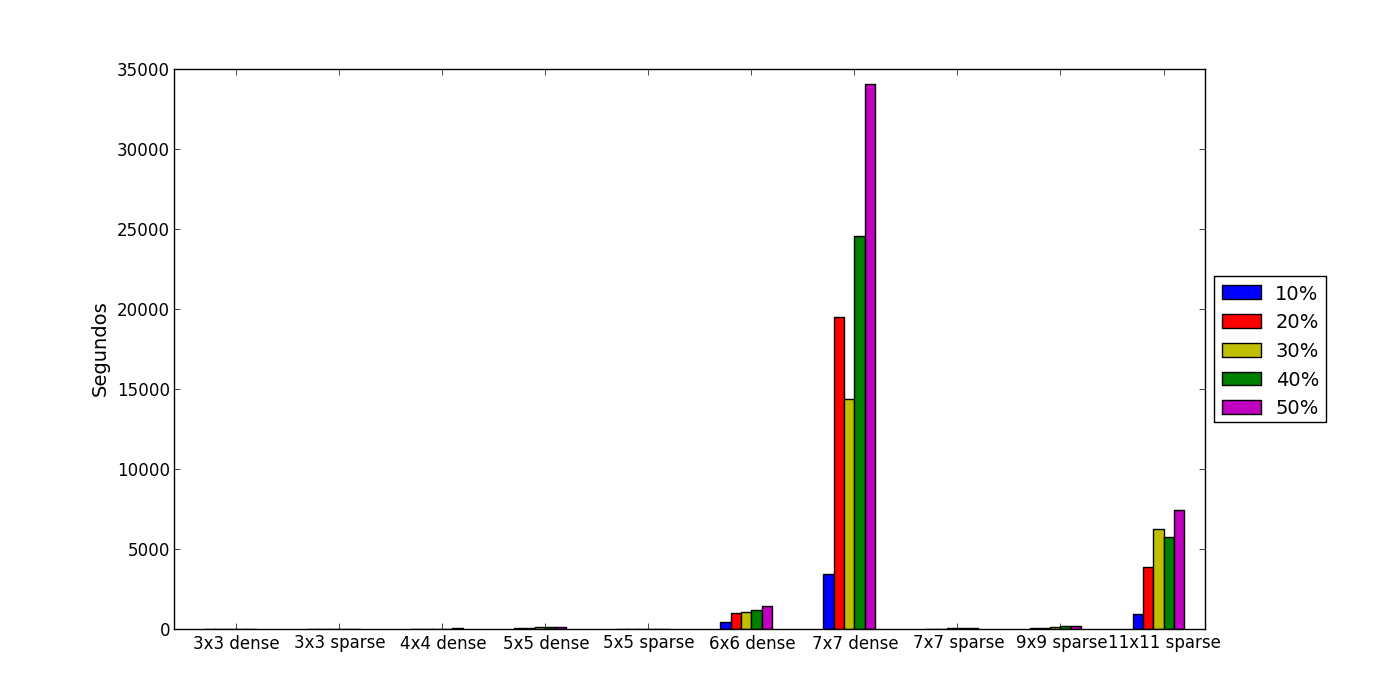
\includegraphics[width=1.2\textwidth]{assets/experiment_charts/TextRegion_paragraph_time.png}}
    \caption{Tempo para treinamento dos operadores de parágrafo}
    \label{fig:paragraph_build_time}
  \end{figure*}

  \begin{figure*}[p]
    \centerline{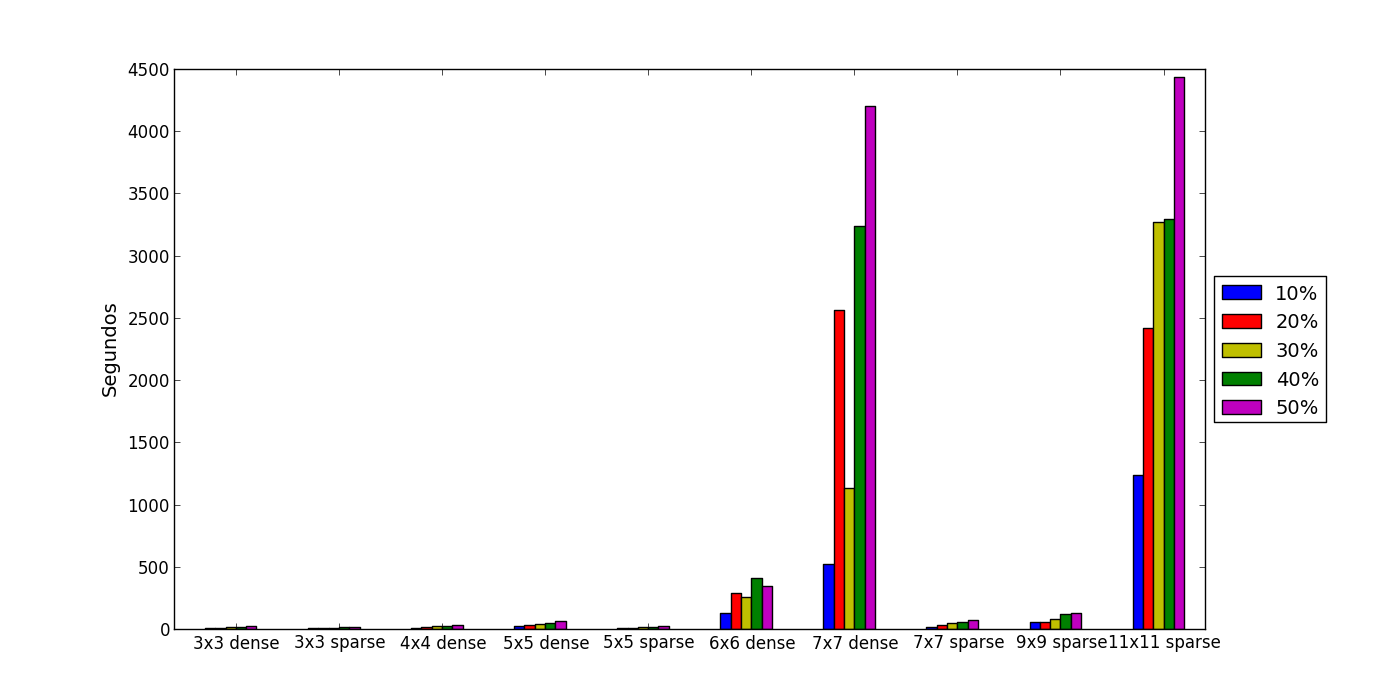
\includegraphics[width=1.2\textwidth]{assets/experiment_charts/TextRegion_heading_time.png}}
    \caption{Tempo para treinamento dos operadores de título}
    \label{fig:heading_build_time}
  \end{figure*}

  \begin{figure*}[p]
    \centerline{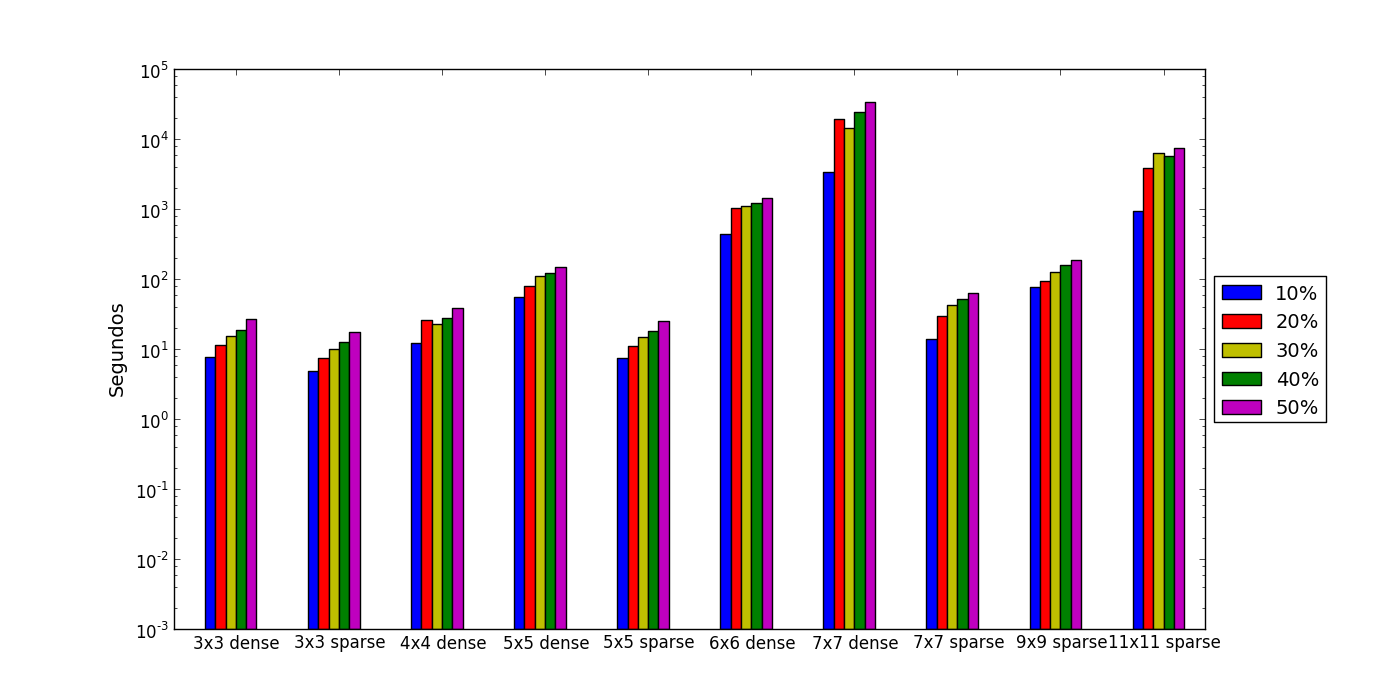
\includegraphics[width=1.2\textwidth]{assets/experiment_charts/TextRegion_paragraph_time_log.png}}
    \caption{Tempo para treinamento dos operadores de parágrafo em escala logarítmica}
    \label{fig:paragraph_build_time_log}
  \end{figure*}

  \begin{figure*}[p]
    \centerline{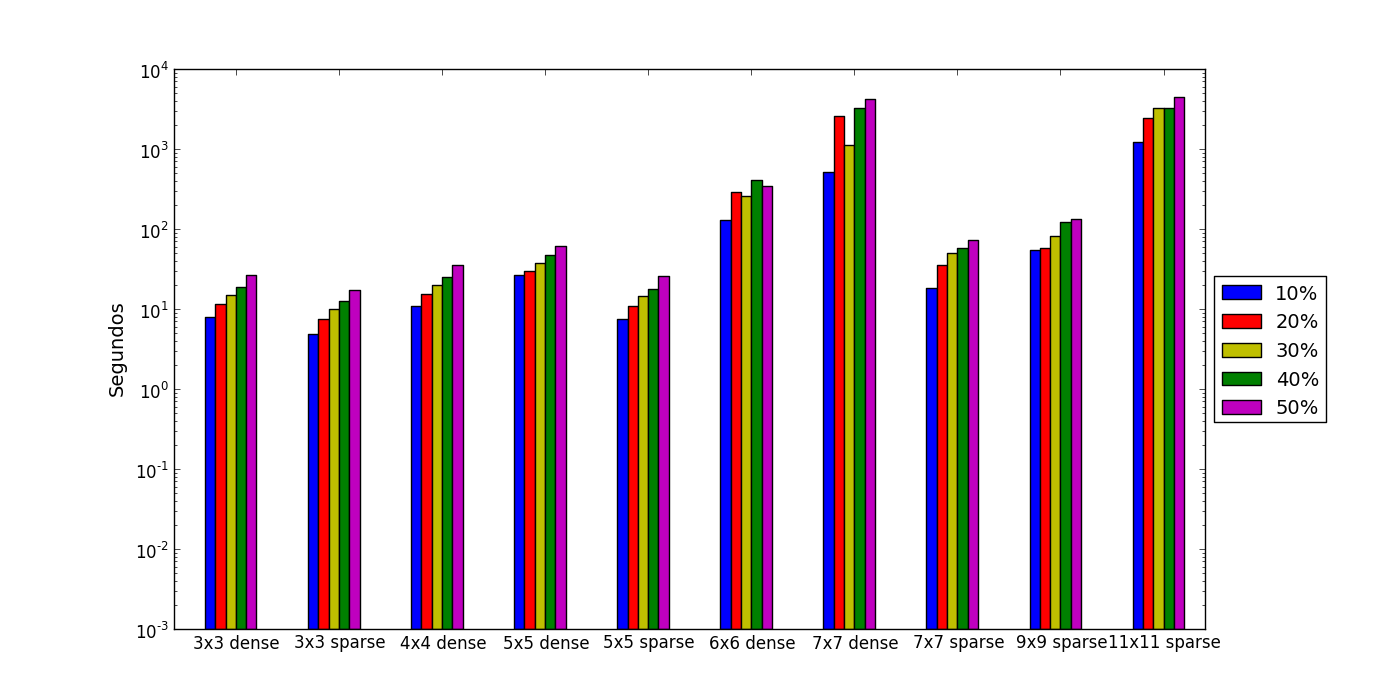
\includegraphics[width=1.2\textwidth]{assets/experiment_charts/TextRegion_heading_time_log.png}}
    \caption{Tempo para treinamento dos operadores de título em escala logarítmica}
    \label{fig:heading_build_time_log}
  \end{figure*}

  \begin{center}
    \begin{table}[p]
      \caption{Média da precisão na classificação de parágrafos do conjunto de dados CACM}
      \begin{tabular}{ l | c c c c c || c c c c c | }
        \cline{2-11}
        & \multicolumn{10}{|c|}{janelas} \\
        \cline{2-11}
        & \multicolumn{5}{c||}{densa} & \multicolumn{5}{c|}{esparsa} \\
        \cline{2-11}
        & 3x3 & 4x4 & 5x5 & 6x6 & 7x7 & 3x3 & 5x5 & 7x7 & 9x9 & 11x11 \\
        \hline
        \multicolumn{1}{|l|}{10\%}& 0.6955& 0.8419& 0.8850& 0.9166& 0.9396& 0.6953& 0.8718& 0.9038& 0.9527& 0.9230\\
        \multicolumn{1}{|l|}{20\%}& 0.8378& 0.8557& 0.8845& 0.8926& 0.9076& 0.8376& 0.8744& 0.8859& 0.9296& 0.9029\\
        \multicolumn{1}{|l|}{30\%}& 0.8383& 0.8690& 0.8911& 0.8979& 0.9141& 0.8376& 0.8751& 0.8921& 0.9345& 0.9047\\
        \multicolumn{1}{|l|}{40\%}& 0.8428& 0.8635& 0.8885& 0.8943& 0.9117& 0.8376& 0.8651& 0.8820& 0.9291& 0.9025\\
        \multicolumn{1}{|l|}{50\%}& 0.8418& 0.8465& 0.8826& 0.8918& 0.9125& 0.8376& 0.8601& 0.8831& 0.9289& 0.9044\\
        \hline  
      \end{tabular}
      \label{tab:cacm_precision_paragraph}
    \end{table}
  \end{center}
    
  \begin{figure*}[p]
    \centerline{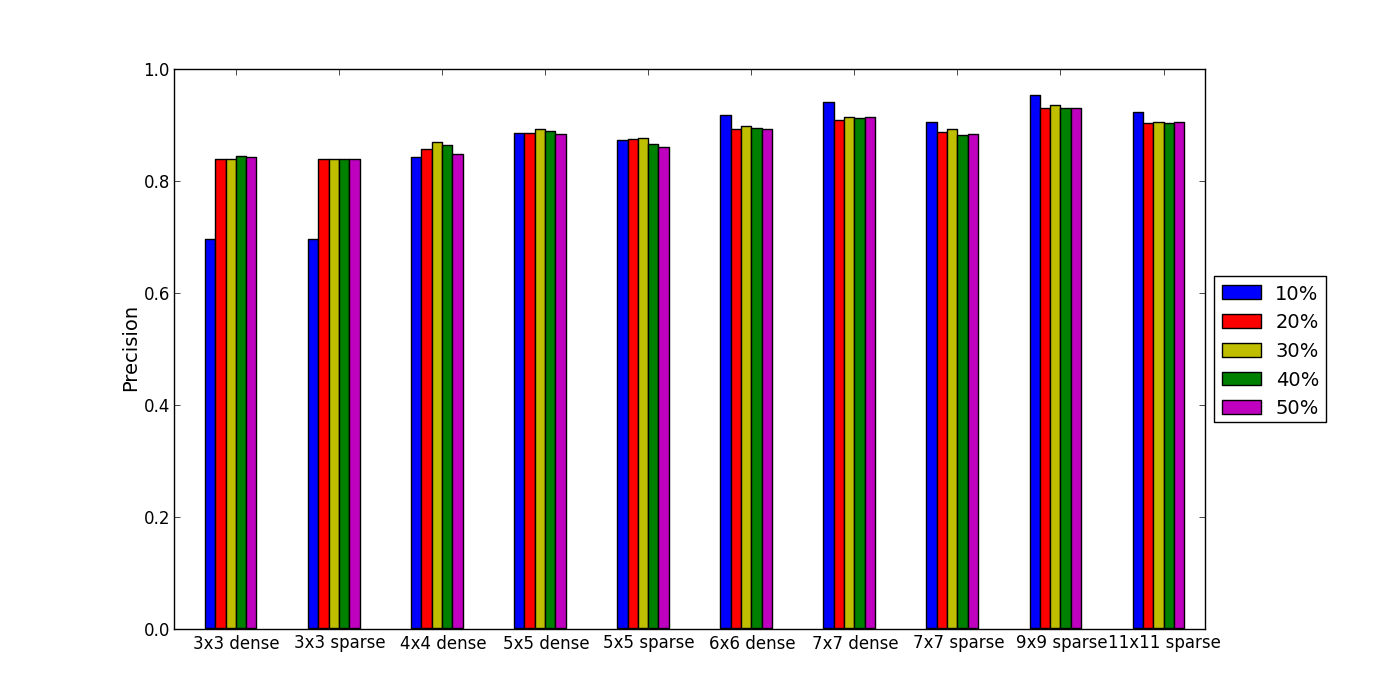
\includegraphics[width=1.2\textwidth]{assets/experiment_charts/cacm_TextRegion_paragraph_precision.png}}
    \caption{CACM: Classificação de parágrafos}
    \label{fig:cacm_TextRegion_paragraph_precision}
  \end{figure*}

  \begin{center}
    \begin{table}[p]
      \caption{Média recall na classificação de parágrafos do conjunto de dados CACM}
      \begin{tabular}{ l | c c c c c || c c c c c | }
        \cline{2-11}
        & \multicolumn{10}{|c|}{janelas} \\
        \cline{2-11}
        & \multicolumn{5}{c||}{densa} & \multicolumn{5}{c|}{esparsa} \\
        \cline{2-11}
        & 3x3 & 4x4 & 5x5 & 6x6 & 7x7 & 3x3 & 5x5 & 7x7 & 9x9 & 11x11 \\
        \hline
        \multicolumn{1}{|l|}{10\%}& 0.9999& 0.9537& 0.9817& 0.9736& 0.9718& 1.0000& 0.9906& 0.9937& 0.9863& 0.9866\\
        \multicolumn{1}{|l|}{20\%}& 0.7796& 0.9461& 0.9778& 0.9686& 0.9677& 0.7781& 0.9894& 0.9944& 0.9823& 0.9829\\
        \multicolumn{1}{|l|}{30\%}& 0.7795& 0.9316& 0.9740& 0.9683& 0.9668& 0.7781& 0.9886& 0.9928& 0.9829& 0.9848\\
        \multicolumn{1}{|l|}{40\%}& 0.7789& 0.9433& 0.9739& 0.9643& 0.9641& 0.7781& 0.9886& 0.9928& 0.9810& 0.9832\\
        \multicolumn{1}{|l|}{50\%}& 0.7796& 0.9591& 0.9879& 0.9802& 0.9781& 0.7781& 0.9939& 0.9953& 0.9884& 0.9896\\
        \hline  
      \end{tabular}
      \label{tab:cacm_recall_paragraph}
    \end{table}
  \end{center}

  \begin{figure*}[p]
    \centerline{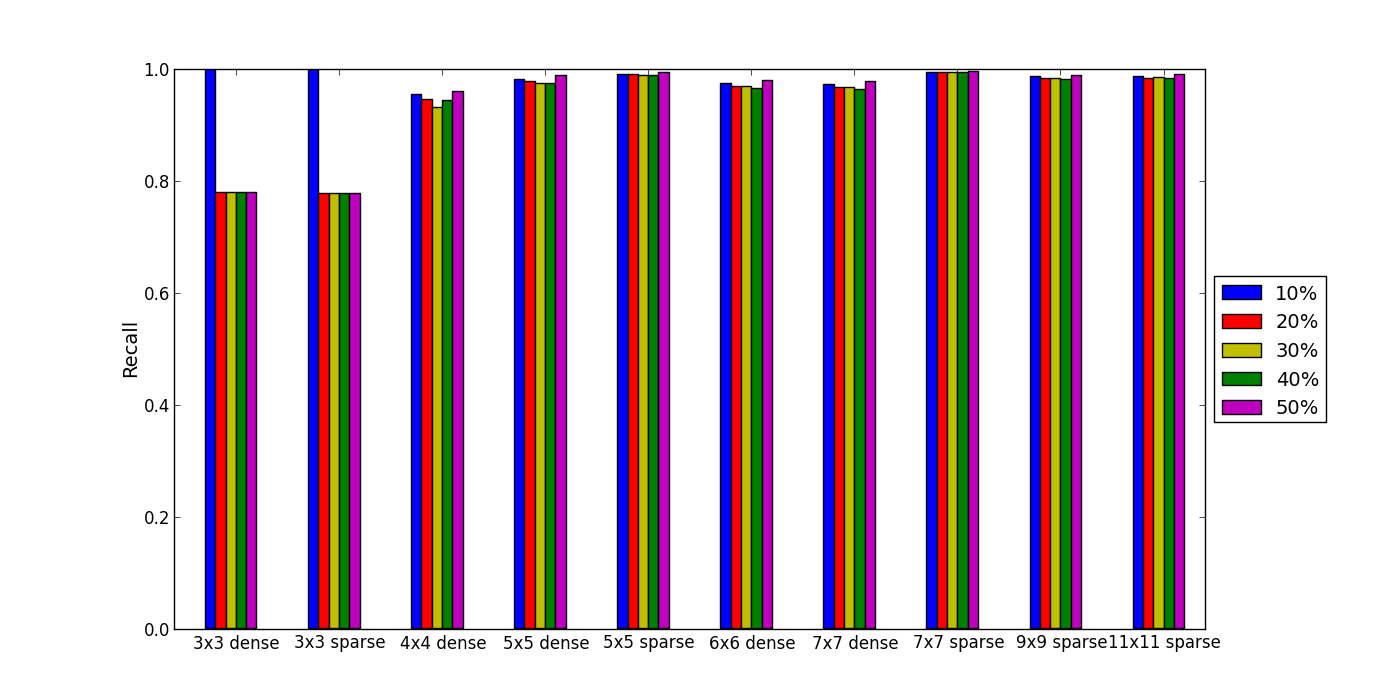
\includegraphics[width=1.2\textwidth]{assets/experiment_charts/cacm_TextRegion_paragraph_recall_or_sensitivity.png}}
    \caption{CACM: Classificação de parágrafos}
    \label{fig:cacm_TextRegion_paragraph_recall_or_sensitivity}
  \end{figure*}

  \begin{center}
    \begin{table}[p]
      \caption{Média F1 na classificação de parágrafos do conjunto de dados CACM}
      \begin{tabular}{ l | c c c c c || c c c c c | }
        \cline{2-11}
        & \multicolumn{10}{|c|}{janelas} \\
        \cline{2-11}
        & \multicolumn{5}{c||}{densa} & \multicolumn{5}{c|}{esparsa} \\
        \cline{2-11}
        & 3x3 & 4x4 & 5x5 & 6x6 & 7x7 & 3x3 & 5x5 & 7x7 & 9x9 & 11x11 \\
        \hline
        \multicolumn{1}{|l|}{10\%}& 0.8088& 0.8932& 0.9304& 0.9440& 0.9553& 0.8087& 0.9268& 0.9462& 0.9691& 0.9534\\
        \multicolumn{1}{|l|}{20\%}& 0.8067& 0.8979& 0.9284& 0.9287& 0.9365& 0.8058& 0.9278& 0.9366& 0.9550& 0.9409\\
        \multicolumn{1}{|l|}{30\%}& 0.8068& 0.8987& 0.9303& 0.9315& 0.9396& 0.8058& 0.9279& 0.9394& 0.9580& 0.9428\\
        \multicolumn{1}{|l|}{40\%}& 0.8087& 0.9010& 0.9288& 0.9277& 0.9370& 0.8058& 0.9221& 0.9337& 0.9542& 0.9409\\
        \multicolumn{1}{|l|}{50\%}& 0.8086& 0.8984& 0.9319& 0.9336& 0.9440& 0.8058& 0.9215& 0.9354& 0.9576& 0.9448\\
        \hline  
      \end{tabular}
      \label{tab:cacm_f1_paragraph}
    \end{table}
  \end{center}

  \begin{figure*}[p]
    \centerline{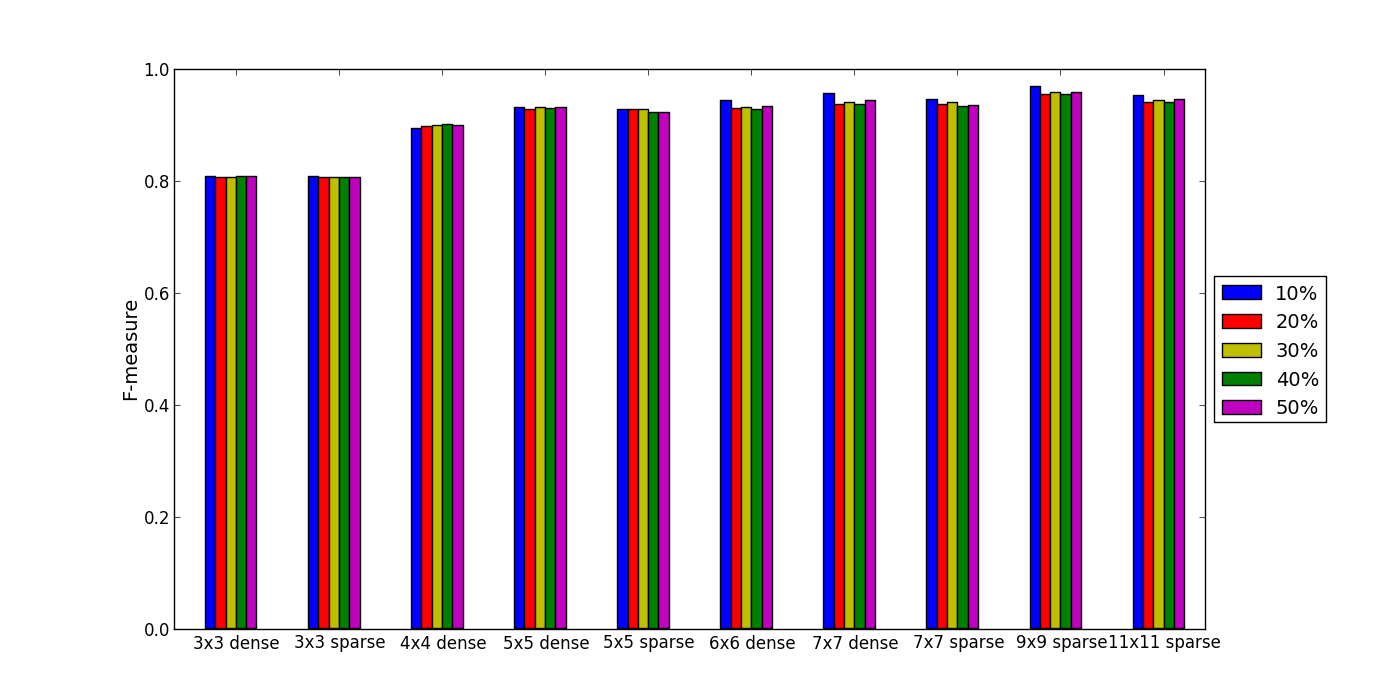
\includegraphics[width=1.2\textwidth]{assets/experiment_charts/cacm_TextRegion_paragraph_f1.png}}
    \caption{CACM: Classificação de parágrafos}
    \label{fig:cacm_TextRegion_paragraph_f1}
  \end{figure*}

  \begin{center}
    \begin{table}[p]
      \caption{Média MCC na classificação de parágrafos do conjunto de dados CACM}
      \begin{tabular}{ l | c c c c c || c c c c c | }
        \cline{2-11}
        & \multicolumn{10}{|c|}{janelas} \\
        \cline{2-11}
        & \multicolumn{5}{c||}{densa} & \multicolumn{5}{c|}{esparsa} \\
        \cline{2-11}
        & 3x3 & 4x4 & 5x5 & 6x6 & 7x7 & 3x3 & 5x5 & 7x7 & 9x9 & 11x11 \\
        \hline
        \multicolumn{1}{|l|}{10\%}& 0.0212& 0.5591& 0.7194& 0.7746& 0.8199& 0.0006& 0.6999& 0.7775& 0.8669& 0.8100\\
        \multicolumn{1}{|l|}{20\%}& 0.3717& 0.5825& 0.7123& 0.7134& 0.7460& 0.3691& 0.7025& 0.7312& 0.8123& 0.7560\\
        \multicolumn{1}{|l|}{30\%}& 0.3726& 0.5940& 0.7205& 0.7276& 0.7621& 0.3691& 0.7022& 0.7434& 0.8261& 0.7671\\
        \multicolumn{1}{|l|}{40\%}& 0.3815& 0.5950& 0.7105& 0.7087& 0.7497& 0.3691& 0.6803& 0.7187& 0.8095& 0.7568\\
        \multicolumn{1}{|l|}{50\%}& 0.3795& 0.5740& 0.7246& 0.7302& 0.7767& 0.3691& 0.6810& 0.7259& 0.8235& 0.7743\\
        \hline  
      \end{tabular}
      \label{tab:cacm_mcc_paragraph}
    \end{table}
  \end{center}

  \begin{figure*}[p]
    \centerline{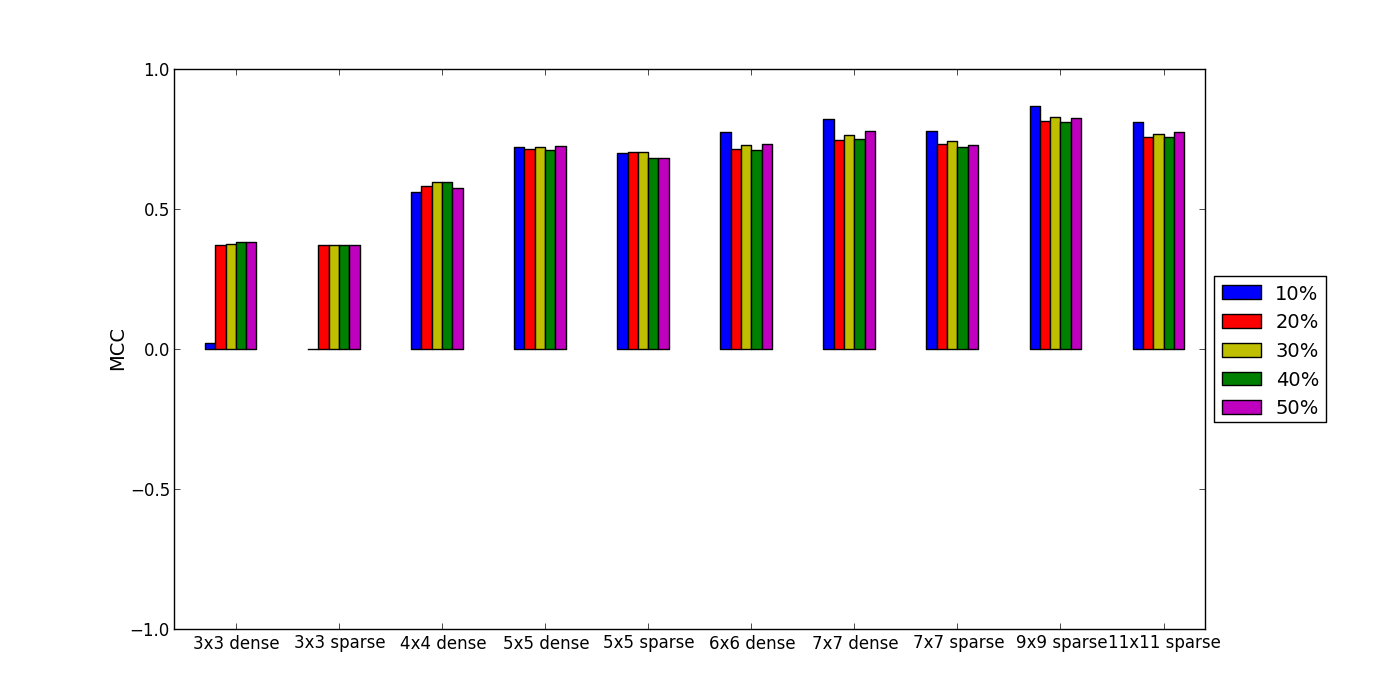
\includegraphics[width=1.2\textwidth]{assets/experiment_charts/cacm_TextRegion_paragraph_mcc.png}}
    \caption{CACM: Classificação de parágrafos}
    \label{fig:cacm_TextRegion_paragraph_mcc}
  \end{figure*}

  \begin{center}
    \begin{table}[p]
      \caption{Média da precisão na classificação de parágrafos do conjunto de dados TIME}
      \begin{tabular}{ l | c c c c c || c c c c c | }
        \cline{2-11}
        & \multicolumn{10}{|c|}{janelas} \\
        \cline{2-11}
        & \multicolumn{5}{c||}{densa} & \multicolumn{5}{c|}{esparsa} \\
        \cline{2-11}
        & 3x3 & 4x4 & 5x5 & 6x6 & 7x7 & 3x3 & 5x5 & 7x7 & 9x9 & 11x11 \\
        \hline
        \multicolumn{1}{|l|}{10\%}& 0.7725& 0.8186& 0.8662& 0.8856& 0.9093& 0.7226& 0.8536& 0.8119& 0.8968& 0.8095\\
        \multicolumn{1}{|l|}{30\%}& 0.7729& 0.8123& 0.8699& 0.9007& 0.9177& 0.7226& 0.8440& 0.8188& 0.9032& 0.8210\\
        \multicolumn{1}{|l|}{40\%}& 0.7466& 0.7997& 0.8655& 0.9008& 0.9211& 0.7077& 0.7858& 0.8155& 0.9044& 0.8271\\
        \multicolumn{1}{|l|}{50\%}& 0.7493& 0.8139& 0.8775& 0.9087& 0.9304& 0.7226& 0.8364& 0.8221& 0.9094& 0.8272\\
        \hline  
      \end{tabular}
      \label{tab:time_precision_paragraph}
    \end{table}
  \end{center}

  \begin{figure*}[p]
    \centerline{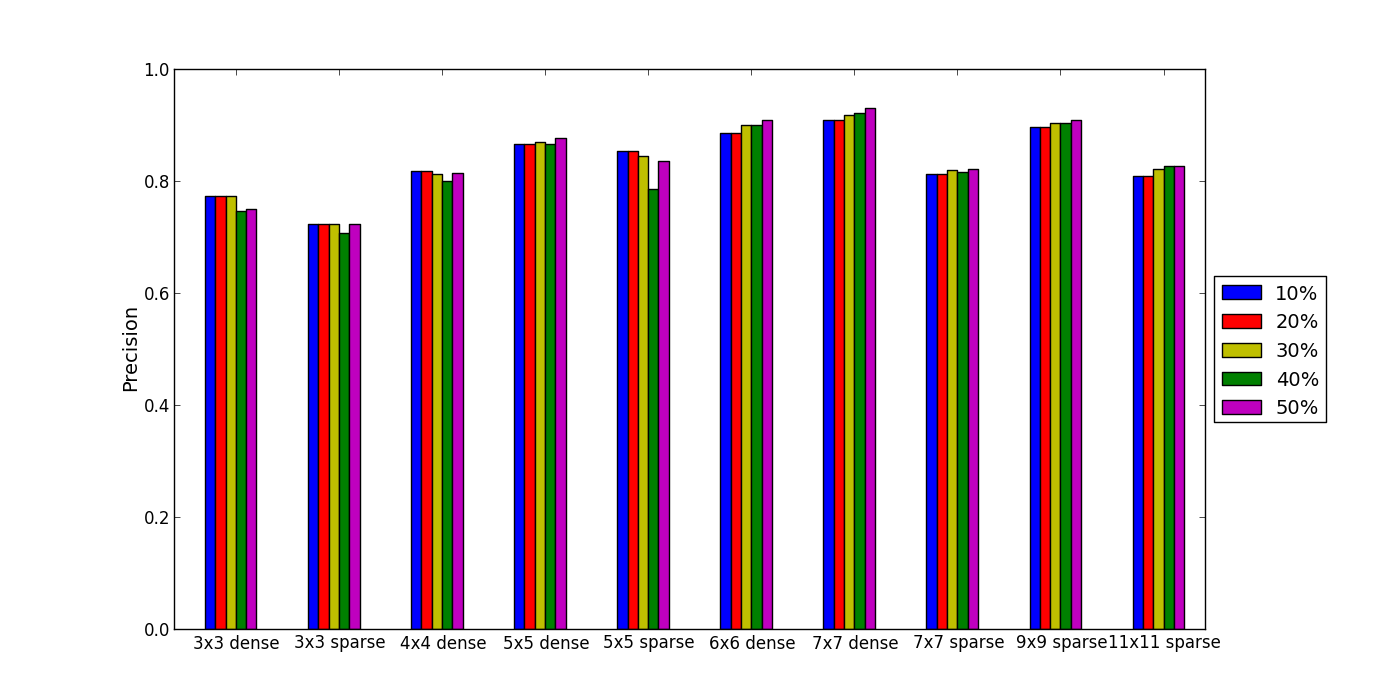
\includegraphics[width=1.2\textwidth]{assets/experiment_charts/time_TextRegion_paragraph_precision.png}}
    \caption{TIME: Classificação de parágrafos}
    \label{fig:time_TextRegion_paragraph_precision}
  \end{figure*}  

  \begin{center}
    \begin{table}[p]
      \caption{Média recall na classificação de parágrafos do conjunto de dados TIME}
      \begin{tabular}{ l | c c c c c || c c c c c | }
        \cline{2-11}
        & \multicolumn{10}{|c|}{janelas} \\
        \cline{2-11}
        & \multicolumn{5}{c||}{densa} & \multicolumn{5}{c|}{esparsa} \\
        \cline{2-11}
        & 3x3 & 4x4 & 5x5 & 6x6 & 7x7 & 3x3 & 5x5 & 7x7 & 9x9 & 11x11 \\
        \hline
        \multicolumn{1}{|l|}{10\%}& 0.6025& 0.7503& 0.7864& 0.7966& 0.8039& 0.7645& 0.6514& 0.9461& 0.8761& 0.9172\\
        \multicolumn{1}{|l|}{30\%}& 0.6011& 0.7712& 0.7990& 0.8170& 0.8286& 0.7645& 0.6825& 0.9489& 0.8939& 0.9263\\
        \multicolumn{1}{|l|}{40\%}& 0.7304& 0.8761& 0.9166& 0.9281& 0.9269& 0.8087& 0.9228& 0.9872& 0.9640& 0.9734\\
        \multicolumn{1}{|l|}{50\%}& 0.7212& 0.8436& 0.8982& 0.9177& 0.9251& 0.7645& 0.7446& 0.9790& 0.9595& 0.9728\\
        \hline  
      \end{tabular}
      \label{tab:time_recall_paragraph}
    \end{table}
  \end{center}

  \begin{figure*}[p]
    \centerline{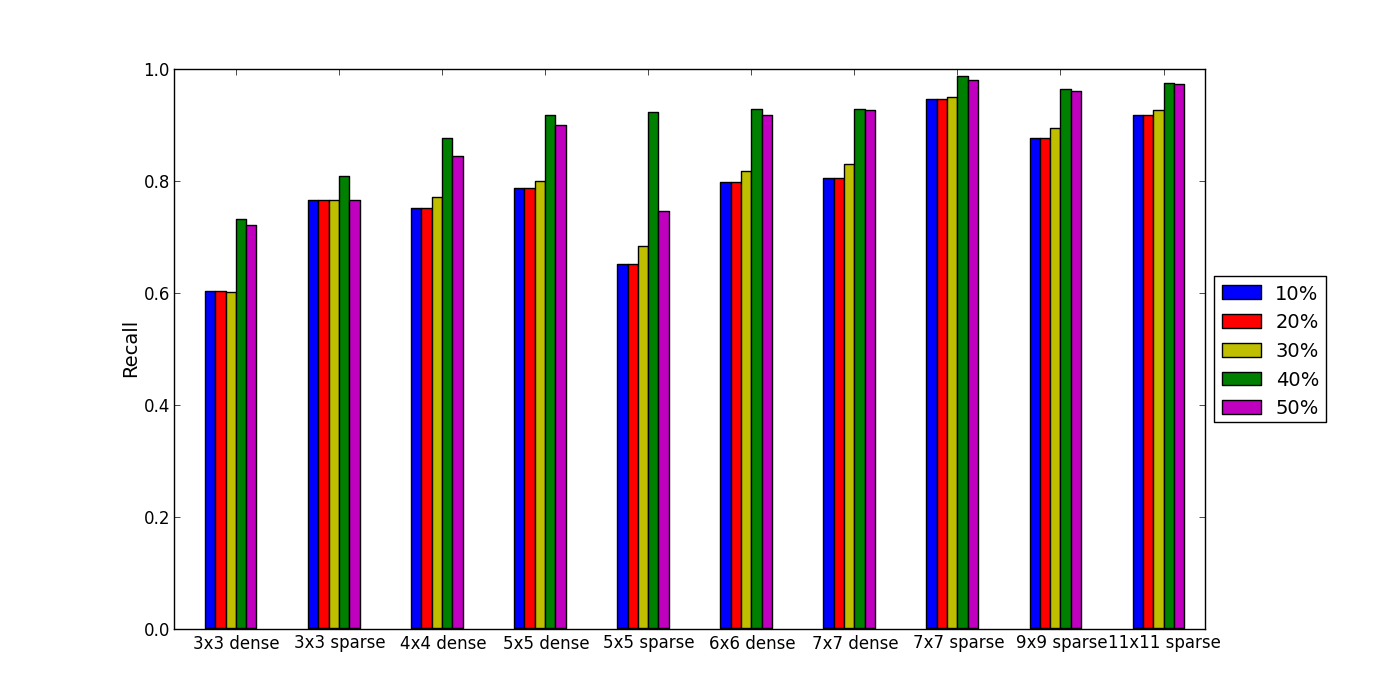
\includegraphics[width=1.2\textwidth]{assets/experiment_charts/time_TextRegion_paragraph_recall_or_sensitivity.png}}
    \caption{TIME: Classificação de parágrafos}
    \label{fig:time_TextRegion_paragraph_recall_or_sensitivity}
  \end{figure*}  

  \begin{center}
    \begin{table}[p]
      \caption{Média F1 na classificação de parágrafos do conjunto de dados TIME}
      \begin{tabular}{ l | c c c c c || c c c c c | }
        \cline{2-11}
        & \multicolumn{10}{|c|}{janelas} \\
        \cline{2-11}
        & \multicolumn{5}{c||}{densa} & \multicolumn{5}{c|}{esparsa} \\
        \cline{2-11}
        & 3x3 & 4x4 & 5x5 & 6x6 & 7x7 & 3x3 & 5x5 & 7x7 & 9x9 & 11x11 \\
        \hline
        \multicolumn{1}{|l|}{10\%}& 0.6757& 0.7819& 0.8230& 0.8374& 0.8519& 0.7418& 0.7373& 0.8733& 0.8857& 0.8594\\
        \multicolumn{1}{|l|}{30\%}& 0.6750& 0.7902& 0.8315& 0.8553& 0.8694& 0.7418& 0.7532& 0.8785& 0.8980& 0.8699\\
        \multicolumn{1}{|l|}{40\%}& 0.7372& 0.8353& 0.8897& 0.9138& 0.9235& 0.7536& 0.8479& 0.8927& 0.9330& 0.8940\\
        \multicolumn{1}{|l|}{50\%}& 0.7338& 0.8276& 0.8868& 0.9123& 0.9270& 0.7418& 0.7869& 0.8932& 0.9335& 0.8937\\
        \hline  
      \end{tabular}
      \label{tab:time_f1_paragraph}
    \end{table}
  \end{center}

  \begin{figure*}[p]
    \centerline{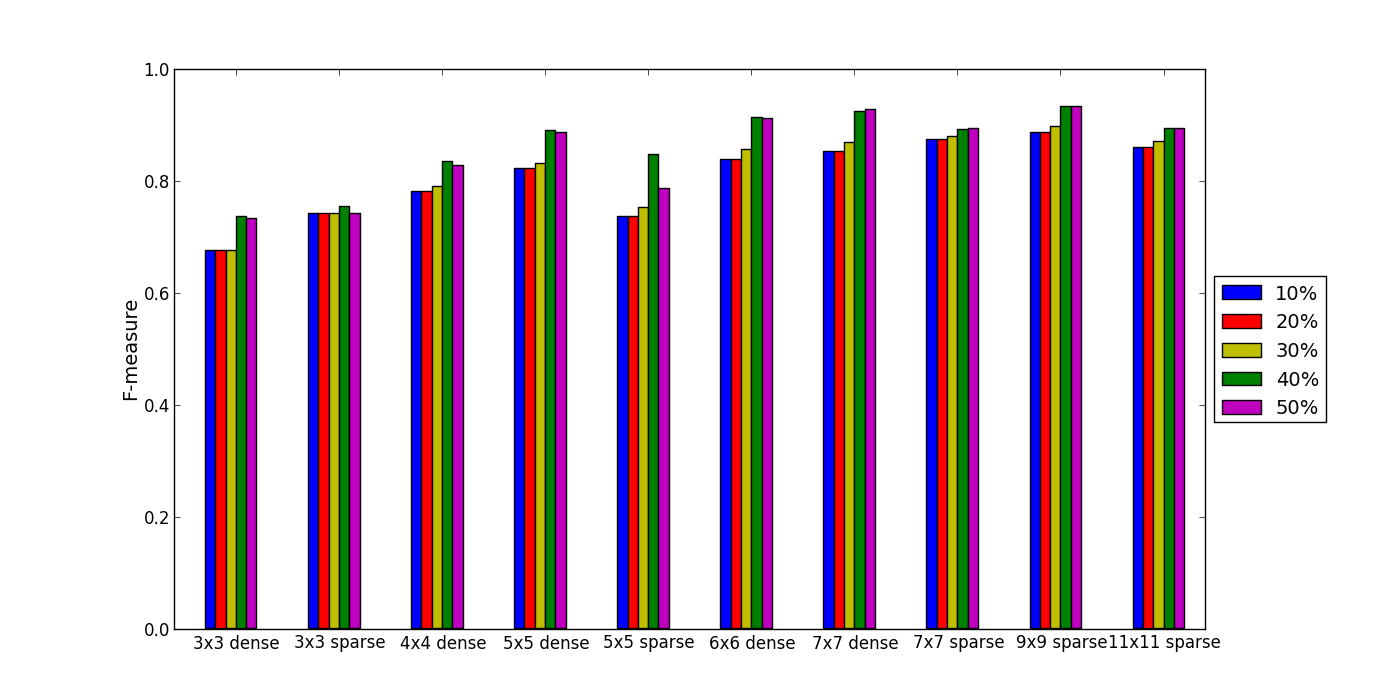
\includegraphics[width=1.2\textwidth]{assets/experiment_charts/time_TextRegion_paragraph_f1.png}}
    \caption{TIME: Classificação de parágrafos}
    \label{fig:time_TextRegion_paragraph_f1}
  \end{figure*}  

  \begin{center}
    \begin{table}[p]
      \caption{Média MCC na classificação de parágrafos do conjunto de dados TIME}
      \begin{tabular}{ l | c c c c c || c c c c c | }
        \cline{2-11}
        & \multicolumn{10}{|c|}{janelas} \\
        \cline{2-11}
        & \multicolumn{5}{c||}{densa} & \multicolumn{5}{c|}{esparsa} \\
        \cline{2-11}
        & 3x3 & 4x4 & 5x5 & 6x6 & 7x7 & 3x3 & 5x5 & 7x7 & 9x9 & 11x11 \\
        \hline
        \multicolumn{1}{|l|}{10\%}& 0.5438& 0.6720& 0.7350& 0.7575& 0.7817& 0.6004& 0.6376& 0.8007& 0.8224& 0.7784\\
        \multicolumn{1}{|l|}{30\%}& 0.5431& 0.6801& 0.7467& 0.7844& 0.8059& 0.6004& 0.6507& 0.8091& 0.8407& 0.7958\\
        \multicolumn{1}{|l|}{40\%}& 0.6010& 0.7393& 0.8253& 0.8642& 0.8799& 0.6137& 0.7601& 0.8352& 0.8939& 0.8362\\
        \multicolumn{1}{|l|}{50\%}& 0.5977& 0.7310& 0.8227& 0.8629& 0.8863& 0.6004& 0.6854& 0.8350& 0.8947& 0.8363\\
        \hline  
      \end{tabular}
      \label{tab:time_mcc_paragraph}
    \end{table}
  \end{center}

  \begin{figure*}[p]
    \centerline{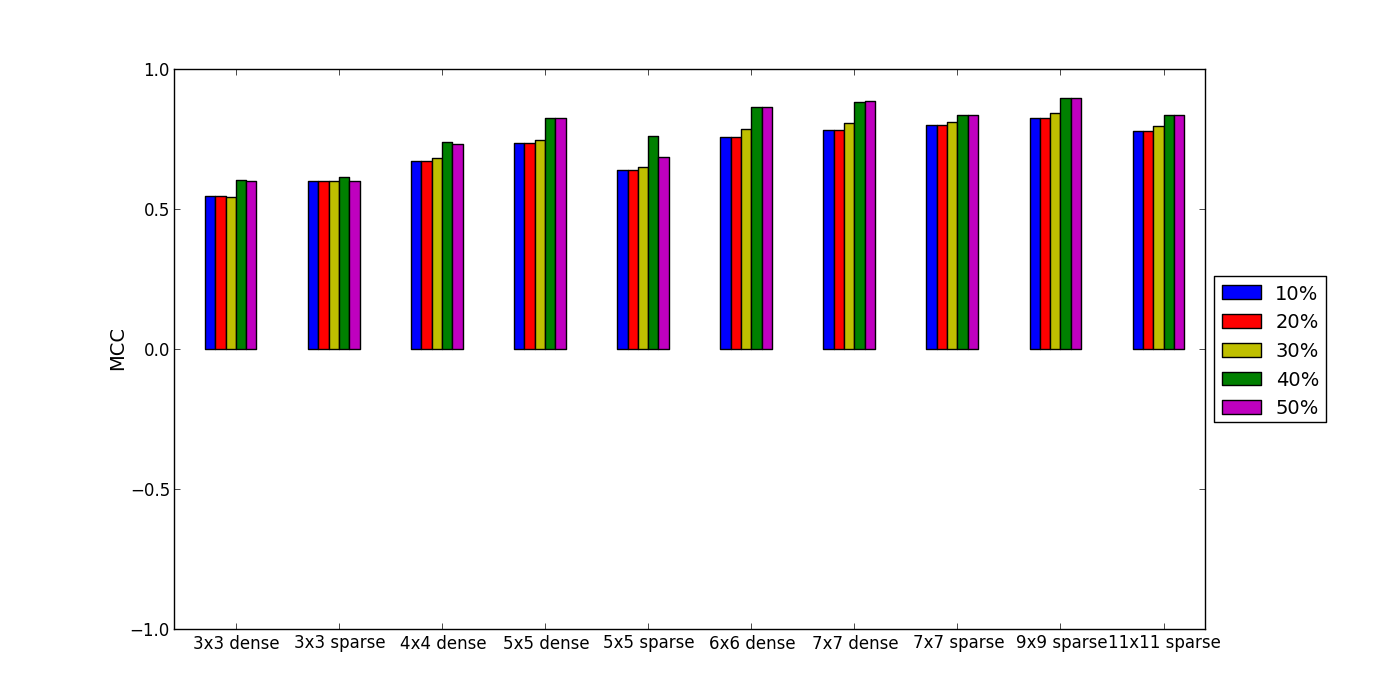
\includegraphics[width=1.2\textwidth]{assets/experiment_charts/time_TextRegion_paragraph_mcc.png}}
    \caption{TIME: Classificação de parágrafos}
    \label{fig:time_TextRegion_paragraph_mcc}
  \end{figure*}  

  \begin{center}
    \begin{table}[p]
      \caption{Média da precisão na classificação de títulos do conjunto de dados CACM}
      \begin{tabular}{ l | c c c c c || c c c c c | }
        \cline{2-11}
        & \multicolumn{10}{|c|}{janelas} \\
        \cline{2-11}
        & \multicolumn{5}{c||}{densa} & \multicolumn{5}{c|}{esparsa} \\
        \cline{2-11}
        & 3x3 & 4x4 & 5x5 & 6x6 & 7x7 & 3x3 & 5x5 & 7x7 & 9x9 & 11x11 \\
        \hline
        \multicolumn{1}{|l|}{10\%}& 0.0000& 0.2115& 0.2198& 0.2301& 0.2335& 0.0467& 0.2413& 0.0910& 0.2802& 0.1275\\
        \multicolumn{1}{|l|}{20\%}& 0.0000& 0.1650& 0.1894& 0.2171& 0.2609& 0.0467& 0.2485& 0.0878& 0.2943& 0.1676\\
        \multicolumn{1}{|l|}{30\%}& 0.0000& 0.1352& 0.1115& 0.2115& 0.2642& 0.0467& 0.2000& 0.0725& 0.3060& 0.1495\\
        \multicolumn{1}{|l|}{40\%}& 0.0000& 0.1518& 0.1381& 0.2146& 0.2637& 0.0467& 0.2000& 0.1006& 0.2945& 0.1653\\
        \multicolumn{1}{|l|}{50\%}& 0.0000& 0.1864& 0.1848& 0.2334& 0.2842& 0.0467& 0.0000& 0.1069& 0.3256& 0.1771\\
        \hline  
      \end{tabular}
      \label{tab:cacm_precision_heading}
    \end{table}
  \end{center}
    
  \begin{figure*}[p]
    \centerline{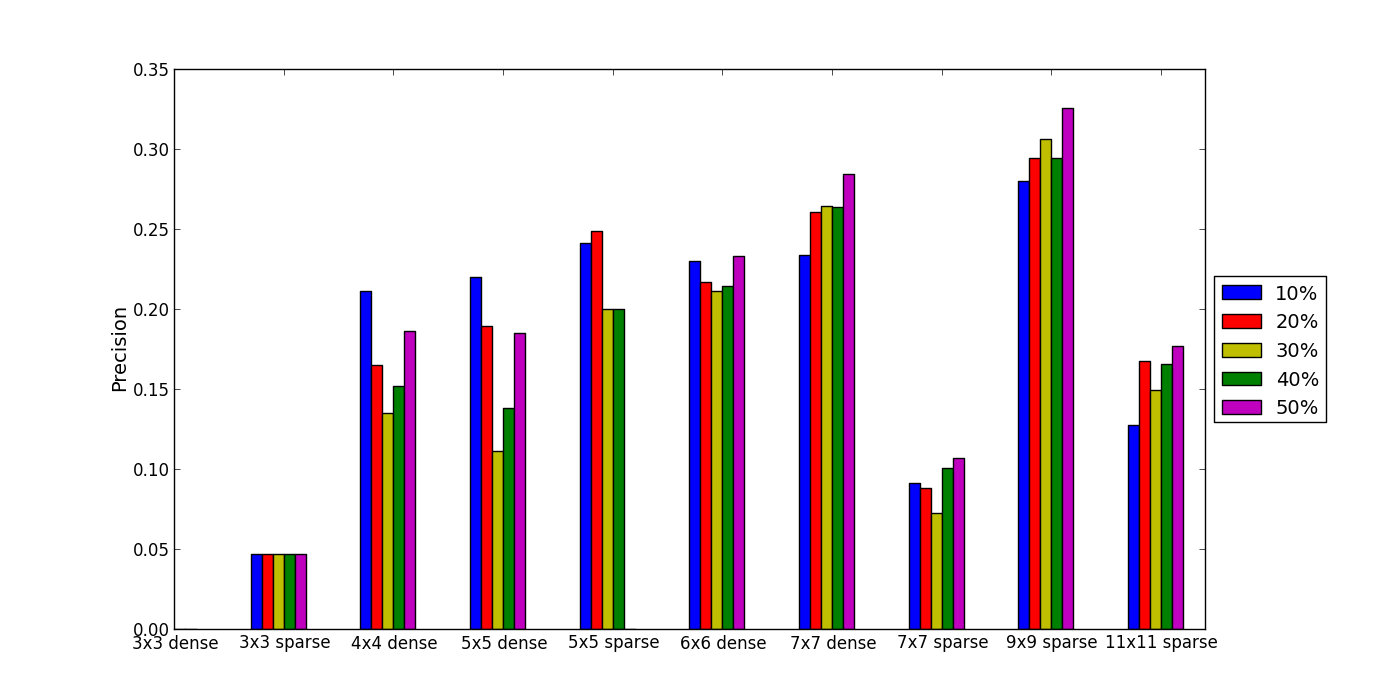
\includegraphics[width=1.2\textwidth]{assets/experiment_charts/cacm_TextRegion_heading_precision.png}}
    \caption{CACM: Classificação de títulos}
    \label{fig:cacm_TextRegion_heading_precision}
  \end{figure*}

  \begin{center}
    \begin{table}[p]
      \caption{Média recall na classificação de títulos do conjunto de dados CACM}
      \begin{tabular}{ l | c c c c c || c c c c c | }
        \cline{2-11}
        & \multicolumn{10}{|c|}{janelas} \\
        \cline{2-11}
        & \multicolumn{5}{c||}{densa} & \multicolumn{5}{c|}{esparsa} \\
        \cline{2-11}
        & 3x3 & 4x4 & 5x5 & 6x6 & 7x7 & 3x3 & 5x5 & 7x7 & 9x9 & 11x11 \\
        \hline
        \multicolumn{1}{|l|}{10\%}& 0.0000& 0.0083& 0.0667& 0.1420& 0.2059& 0.1731& 0.0130& 0.2912& 0.2506& 0.3712\\
        \multicolumn{1}{|l|}{20\%}& 0.0000& 0.0014& 0.0382& 0.1209& 0.2411& 0.1731& 0.0028& 0.2550& 0.2931& 0.4557\\
        \multicolumn{1}{|l|}{30\%}& 0.0000& 0.0003& 0.0049& 0.0539& 0.1683& 0.1731& 0.0000& 0.1883& 0.2081& 0.3980\\
        \multicolumn{1}{|l|}{40\%}& 0.0000& 0.0002& 0.0167& 0.1091& 0.2598& 0.1731& 0.0000& 0.2777& 0.2925& 0.4640\\
        \multicolumn{1}{|l|}{50\%}& 0.0000& 0.0002& 0.0269& 0.1113& 0.2709& 0.1731& 0.0000& 0.2866& 0.3531& 0.4885\\
        \hline  
      \end{tabular}
      \label{tab:cacm_recall_heading}
    \end{table}
  \end{center}

  \begin{figure*}[p]
    \centerline{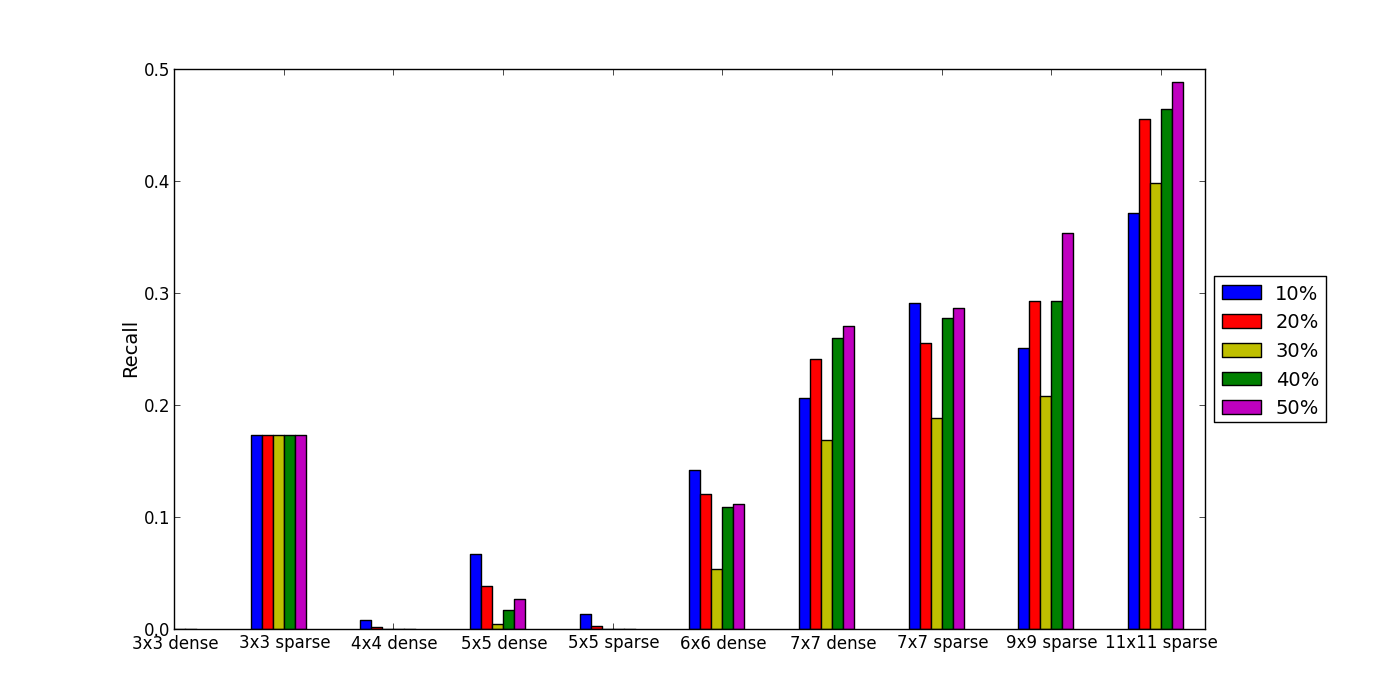
\includegraphics[width=1.2\textwidth]{assets/experiment_charts/cacm_TextRegion_heading_recall_or_sensitivity.png}}
    \caption{CACM: Classificação de títulos}
    \label{fig:cacm_TextRegion_heading_recall_or_sensitivity}
  \end{figure*}

  \begin{center}
    \begin{table}[p]
      \caption{Média F1 na classificação de títulos do conjunto de dados CACM}
      \begin{tabular}{ l | c c c c c || c c c c c | }
        \cline{2-11}
        & \multicolumn{10}{|c|}{janelas} \\
        \cline{2-11}
        & \multicolumn{5}{c||}{densa} & \multicolumn{5}{c|}{esparsa} \\
        \cline{2-11}
        & 3x3 & 4x4 & 5x5 & 6x6 & 7x7 & 3x3 & 5x5 & 7x7 & 9x9 & 11x11 \\
        \hline
        \multicolumn{1}{|l|}{10\%}& 0.0000& 0.0152& 0.0869& 0.1428& 0.1766& 0.0601& 0.0234& 0.1119& 0.2094& 0.1510\\
        \multicolumn{1}{|l|}{20\%}& 0.0000& 0.0028& 0.0560& 0.1311& 0.2161& 0.0601& 0.0054& 0.1074& 0.2677& 0.2116\\
        \multicolumn{1}{|l|}{30\%}& 0.0000& 0.0005& 0.0088& 0.0742& 0.1799& 0.0601& 0.0000& 0.0838& 0.2308& 0.1858\\
        \multicolumn{1}{|l|}{40\%}& 0.0000& 0.0004& 0.0265& 0.1252& 0.2319& 0.0601& 0.0000& 0.1234& 0.2731& 0.2125\\
        \multicolumn{1}{|l|}{50\%}& 0.0000& 0.0004& 0.0429& 0.1331& 0.2481& 0.0601& 0.0000& 0.1302& 0.3169& 0.2259\\
        \hline  
      \end{tabular}
      \label{tab:cacm_f1_heading}
    \end{table}
  \end{center}

  \begin{figure*}[p]
    \centerline{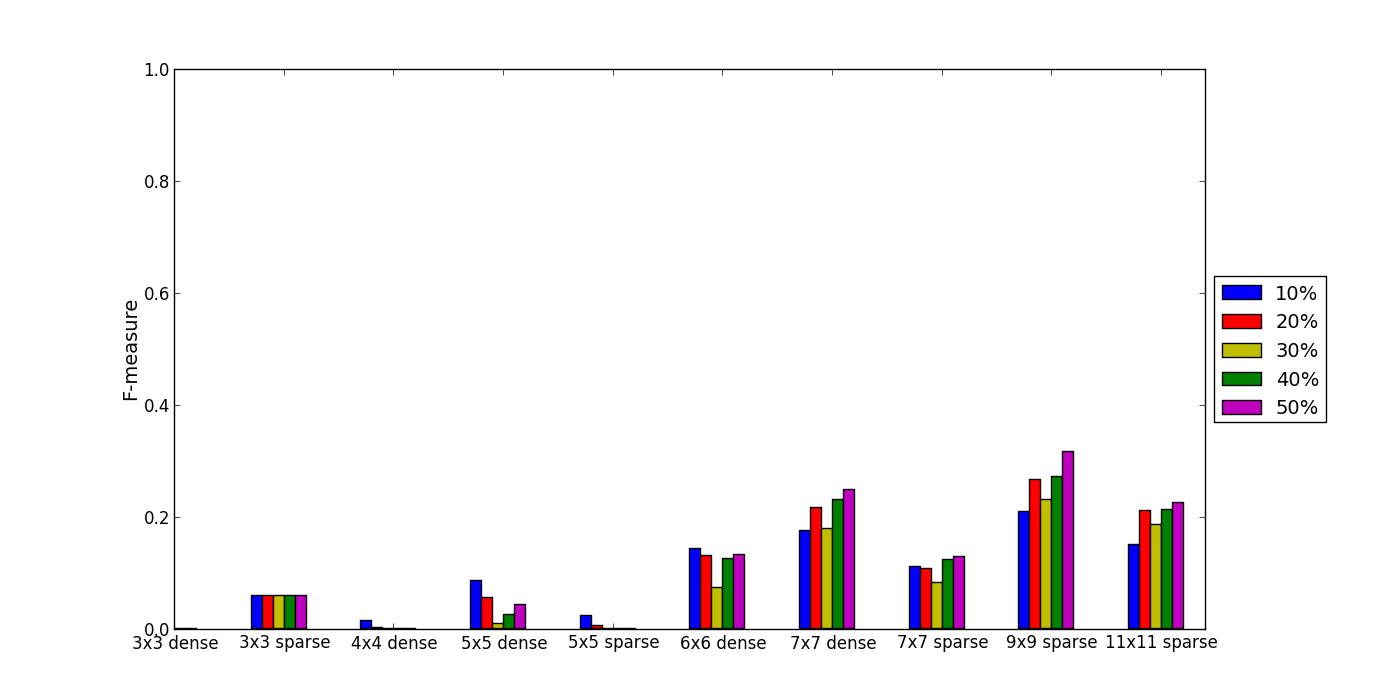
\includegraphics[width=1.2\textwidth]{assets/experiment_charts/cacm_TextRegion_heading_f1.png}}
    \caption{CACM: Classificação de títulos}
    \label{fig:cacm_TextRegion_heading_f1}
  \end{figure*}

  \begin{center}
    \begin{table}[p]
      \caption{Média MCC na classificação de títulos do conjunto de dados CACM}
      \begin{tabular}{ l | c c c c c || c c c c c | }
        \cline{2-11}
        & \multicolumn{10}{|c|}{janelas} \\
        \cline{2-11}
        & \multicolumn{5}{c||}{densa} & \multicolumn{5}{c|}{esparsa} \\
        \cline{2-11}
        & 3x3 & 4x4 & 5x5 & 6x6 & 7x7 & 3x3 & 5x5 & 7x7 & 9x9 & 11x11 \\
        \hline
        \multicolumn{1}{|l|}{10\%}& 0.0000& 0.0243& 0.0739& 0.1184& 0.1484& -0.0879& 0.0357& 0.0239& 0.1958& 0.0964\\
        \multicolumn{1}{|l|}{20\%}& 0.0000& 0.0078& 0.0508& 0.1065& 0.1849& -0.0879& 0.0176& 0.0117& 0.2342& 0.1640\\
        \multicolumn{1}{|l|}{30\%}& 0.0000& 0.0020& 0.0058& 0.0676& 0.1551& -0.0879& 0.0006& -0.0159& 0.2023& 0.1264\\
        \multicolumn{1}{|l|}{40\%}& 0.0000& 0.0024& 0.0203& 0.1003& 0.1975& -0.0879& 0.0008& 0.0319& 0.2372& 0.1637\\
        \multicolumn{1}{|l|}{50\%}& 0.0000& 0.0033& 0.0416& 0.1115& 0.2162& -0.0879& 0.0000& 0.0435& 0.2838& 0.1851\\
        \hline  
      \end{tabular}
      \label{tab:cacm_mcc_heading}
    \end{table}
  \end{center}

  \begin{figure*}[p]
    \centerline{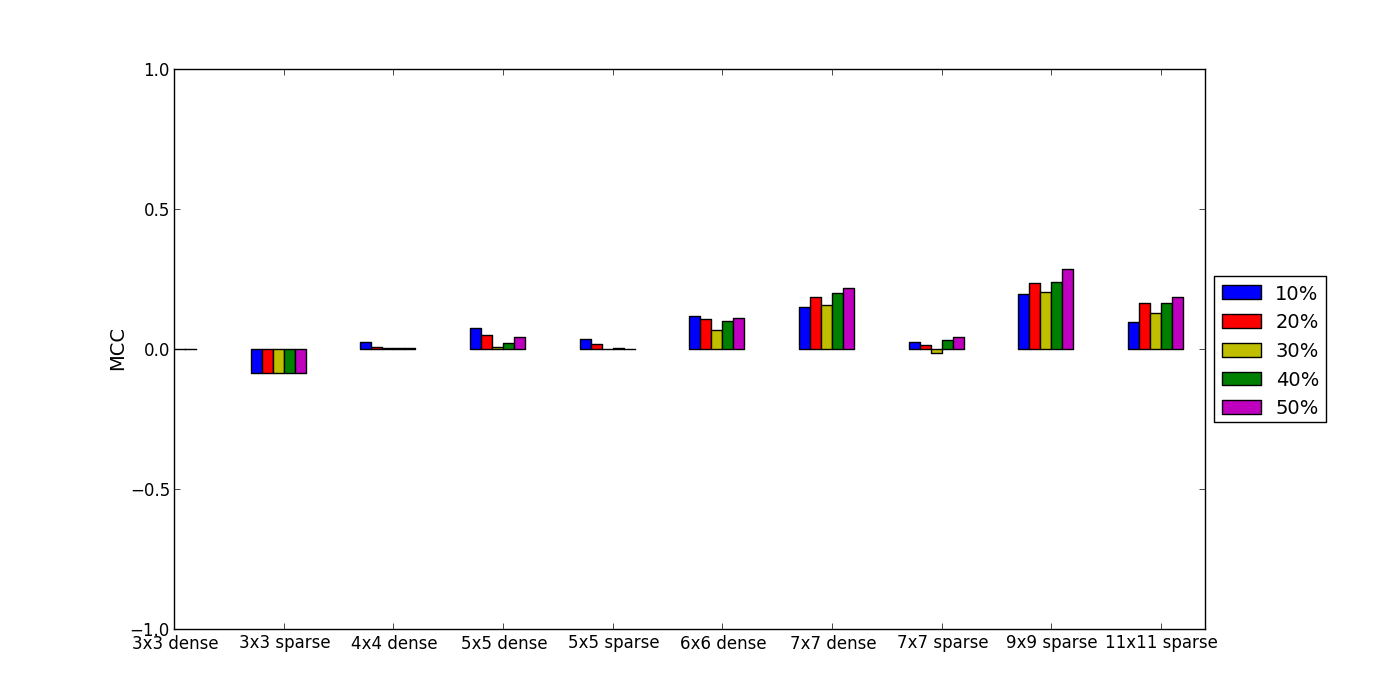
\includegraphics[width=1.2\textwidth]{assets/experiment_charts/cacm_TextRegion_heading_mcc.png}}
    \caption{CACM: Classificação de títulos}
    \label{fig:cacm_TextRegion_heading_mcc}
  \end{figure*}

  \begin{center}
    \begin{table}[p]
      \caption{Média da precisão na classificação de títulos do conjunto de dados TIME}
      \begin{tabular}{ l | c c c c c || c c c c c | }
        \cline{2-11}
        & \multicolumn{10}{|c|}{janelas} \\
        \cline{2-11}
        & \multicolumn{5}{c||}{densa} & \multicolumn{5}{c|}{esparsa} \\
        \cline{2-11}
        & 3x3 & 4x4 & 5x5 & 6x6 & 7x7 & 3x3 & 5x5 & 7x7 & 9x9 & 11x11 \\
        \hline
        \multicolumn{1}{|l|}{10\%}& 0.0000& 0.0000& 0.0020& 0.0571& 0.0776& 0.0189& 0.0000& 0.0232& 0.0510& 0.0277\\
        \multicolumn{1}{|l|}{30\%}& 0.0000& 0.0000& 0.0018& 0.0063& 0.0137& 0.0189& 0.0000& 0.0227& 0.0151& 0.0217\\
        \multicolumn{1}{|l|}{40\%}& 0.0000& 0.0000& 0.0081& 0.0203& 0.0447& 0.0189& 0.0000& 0.0271& 0.0600& 0.0297\\
        \multicolumn{1}{|l|}{50\%}& 0.0000& 0.0147& 0.0122& 0.0495& 0.0721& 0.0189& 0.0000& 0.0274& 0.1172& 0.0341\\
        \hline  
      \end{tabular}
      \label{tab:time_precision_heading}
    \end{table}
  \end{center}
    
  \begin{figure*}[p]
    \centerline{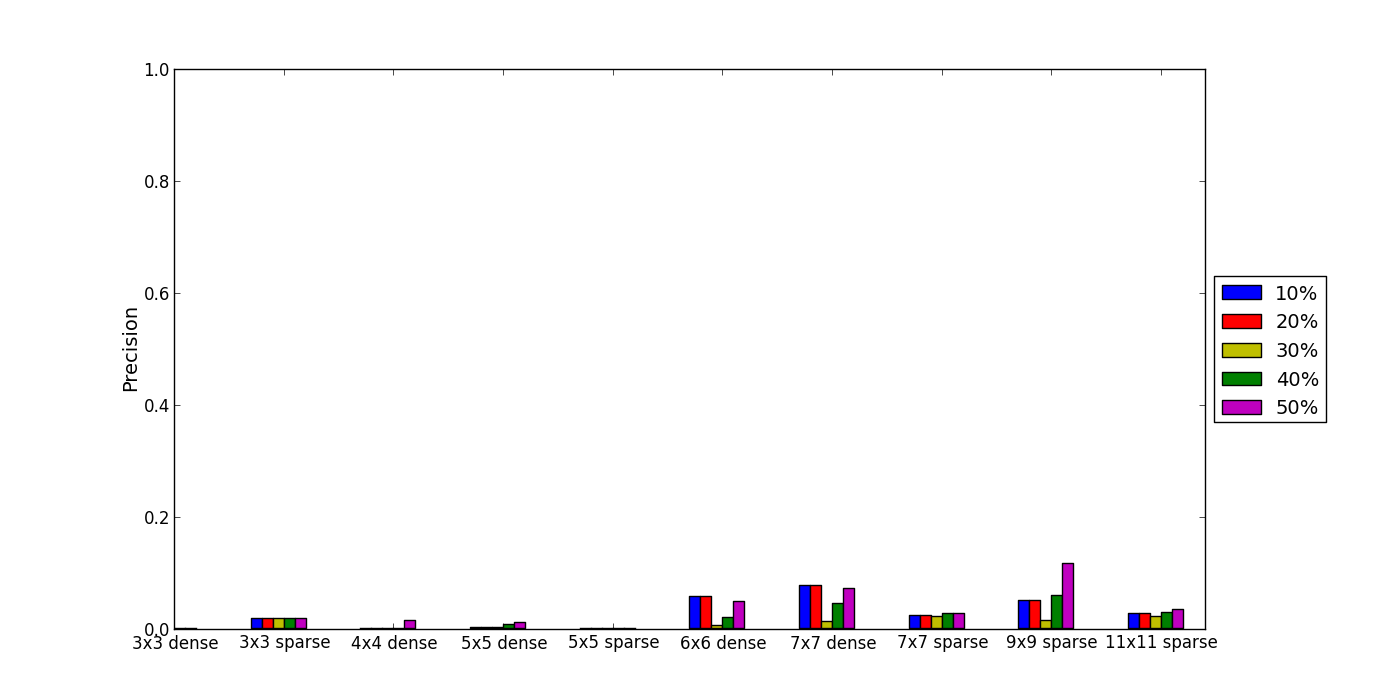
\includegraphics[width=1.2\textwidth]{assets/experiment_charts/time_TextRegion_heading_precision.png}}
    \caption{TIME: Classificação de títulos}
    \label{fig:time_TextRegion_heading_precision}
  \end{figure*}

  \begin{center}
    \begin{table}[p]
      \caption{Média recall na classificação de títulos do conjunto de dados TIME}
      \begin{tabular}{ l | c c c c c || c c c c c | }
        \cline{2-11}
        & \multicolumn{10}{|c|}{janelas} \\
        \cline{2-11}
        & \multicolumn{5}{c||}{densa} & \multicolumn{5}{c|}{esparsa} \\
        \cline{2-11}
        & 3x3 & 4x4 & 5x5 & 6x6 & 7x7 & 3x3 & 5x5 & 7x7 & 9x9 & 11x11 \\
        \hline
        \multicolumn{1}{|l|}{10\%}& 0.0000& 0.0000& 0.0007& 0.0610& 0.1410& 0.1786& 0.0000& 0.1600& 0.0451& 0.2089\\
        \multicolumn{1}{|l|}{30\%}& 0.0000& 0.0000& 0.0004& 0.0053& 0.0166& 0.1786& 0.0000& 0.1558& 0.0108& 0.1598\\
        \multicolumn{1}{|l|}{40\%}& 0.0000& 0.0000& 0.0001& 0.0046& 0.0210& 0.1786& 0.0000& 0.1626& 0.0138& 0.1821\\
        \multicolumn{1}{|l|}{50\%}& 0.0000& 0.0000& 0.0003& 0.0056& 0.0256& 0.1786& 0.0000& 0.1607& 0.0111& 0.1943\\
        \hline  
      \end{tabular}
      \label{tab:time_recall_heading}
    \end{table}
  \end{center}

  \begin{figure*}[p]
    \centerline{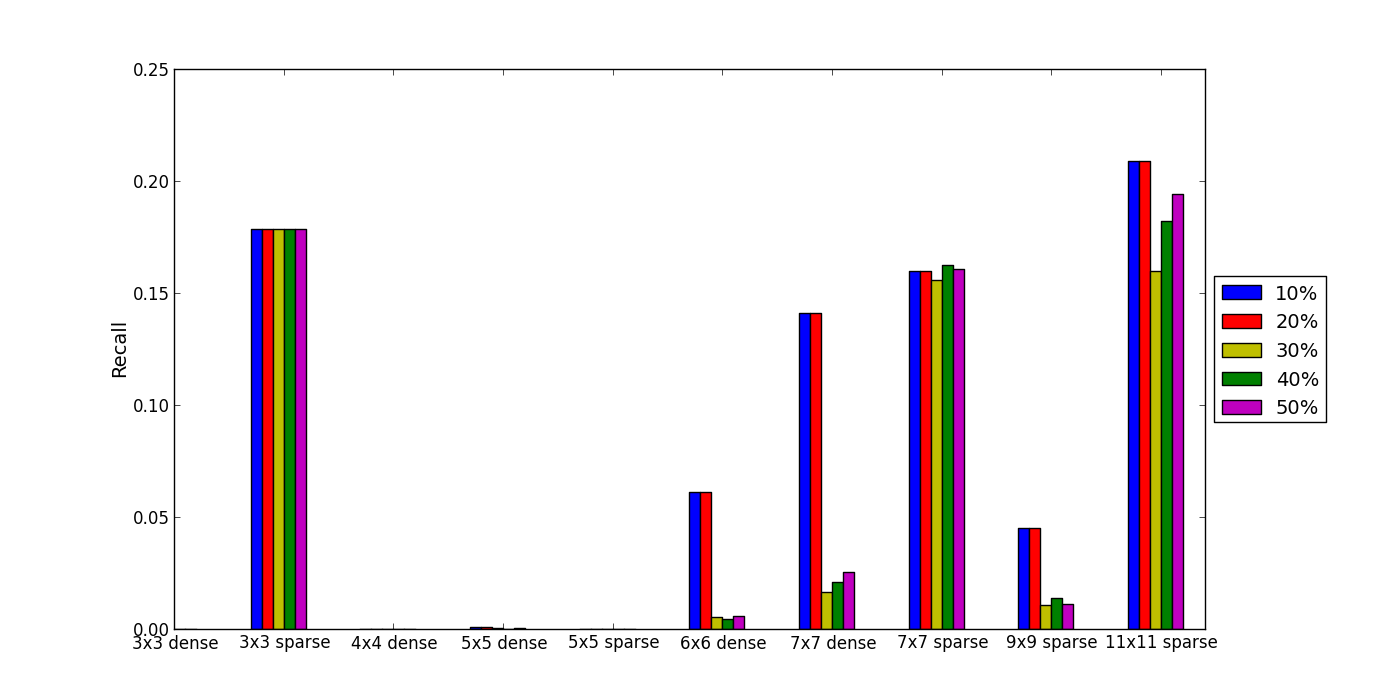
\includegraphics[width=1.2\textwidth]{assets/experiment_charts/time_TextRegion_heading_recall_or_sensitivity.png}}
    \caption{TIME: Classificação de títulos}
    \label{fig:time_TextRegion_heading_recall_or_sensitivity}
  \end{figure*}

  \begin{center}
    \begin{table}[p]
      \caption{Média F1 na classificação de títulos do conjunto de dados TIME}
      \begin{tabular}{ l | c c c c c || c c c c c | }
        \cline{2-11}
        & \multicolumn{10}{|c|}{janelas} \\
        \cline{2-11}
        & \multicolumn{5}{c||}{densa} & \multicolumn{5}{c|}{esparsa} \\
        \cline{2-11}
        & 3x3 & 4x4 & 5x5 & 6x6 & 7x7 & 3x3 & 5x5 & 7x7 & 9x9 & 11x11 \\
        \hline
        \multicolumn{1}{|l|}{10\%}& 0.0000& 0.0000& 0.0010& 0.0568& 0.0966& 0.0331& 0.0000& 0.0392& 0.0451& 0.0476\\
        \multicolumn{1}{|l|}{30\%}& 0.0000& 0.0000& 0.0007& 0.0056& 0.0146& 0.0331& 0.0000& 0.0383& 0.0123& 0.0371\\
        \multicolumn{1}{|l|}{40\%}& 0.0000& 0.0000& 0.0003& 0.0073& 0.0272& 0.0331& 0.0000& 0.0449& 0.0214& 0.0494\\
        \multicolumn{1}{|l|}{50\%}& 0.0000& 0.0000& 0.0005& 0.0099& 0.0367& 0.0331& 0.0000& 0.0452& 0.0199& 0.0562\\
        \hline  
      \end{tabular}
      \label{tab:time_f1_heading}
    \end{table}
  \end{center}

  \begin{figure*}[p]
    \centerline{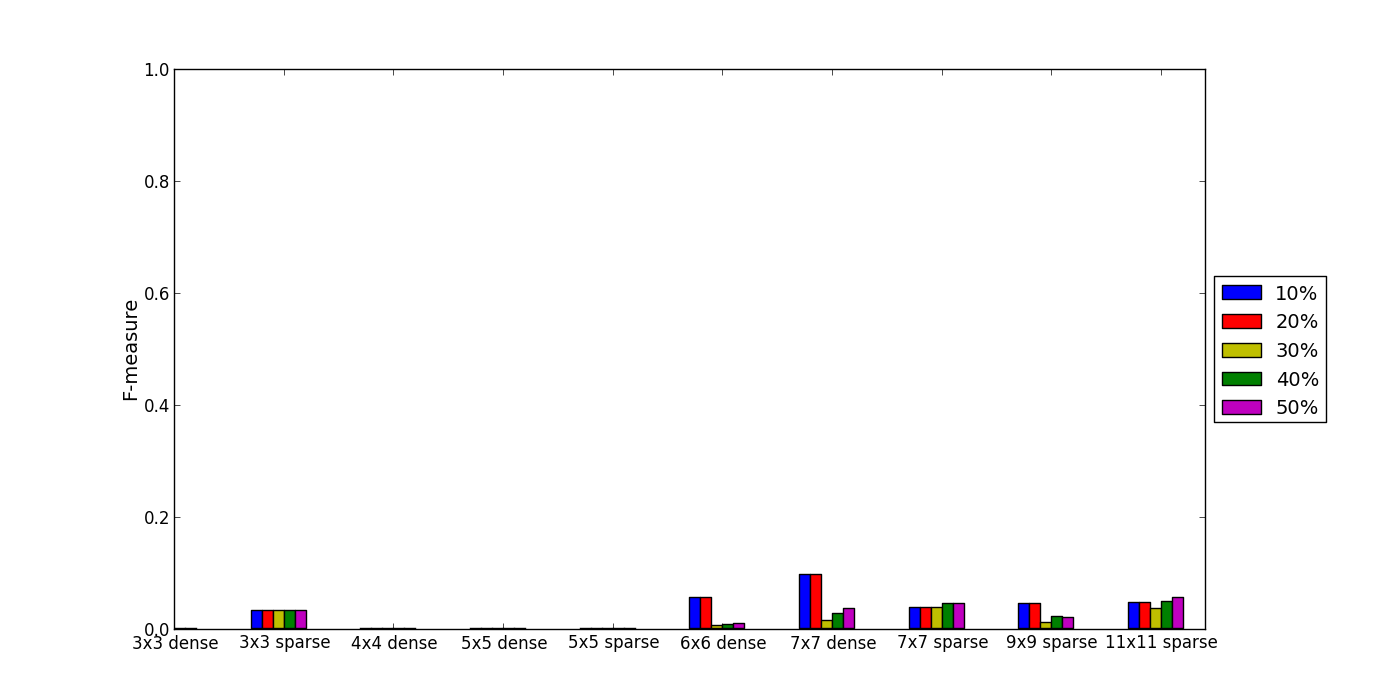
\includegraphics[width=1.2\textwidth]{assets/experiment_charts/time_TextRegion_heading_f1.png}}
    \caption{TIME: Classificação de títulos}
    \label{fig:time_TextRegion_heading_f1}
  \end{figure*}

  \begin{center}
    \begin{table}[p]
      \caption{Média MCC na classificação de títulos do conjunto de dados TIME}
      \begin{tabular}{ l | c c c c c || c c c c c | }
        \cline{2-11}
        & \multicolumn{10}{|c|}{janelas} \\
        \cline{2-11}
        & \multicolumn{5}{c||}{densa} & \multicolumn{5}{c|}{esparsa} \\
        \cline{2-11}
        & 3x3 & 4x4 & 5x5 & 6x6 & 7x7 & 3x3 & 5x5 & 7x7 & 9x9 & 11x11 \\
        \hline
        \multicolumn{1}{|l|}{10\%}& 0.0000& -0.0015& -0.0147& 0.0281& 0.0649& -0.0371& 0.0000& -0.0177& 0.0202& -0.0050\\
        \multicolumn{1}{|l|}{30\%}& 0.0000& -0.0014& -0.0122& -0.0186& -0.0148& -0.0371& 0.0000& -0.0190& -0.0087& -0.0215\\
        \multicolumn{1}{|l|}{40\%}& 0.0000& 0.0000& -0.0024& -0.0027& 0.0109& -0.0371& 0.0000& -0.0061& 0.0151& 0.0018\\
        \multicolumn{1}{|l|}{50\%}& 0.0000& -0.0001& -0.0015& 0.0069& 0.0251& -0.0371& 0.0000& -0.0053& 0.0263& 0.0121\\
        \hline  
      \end{tabular}
      \label{tab:time_mcc_heading}
    \end{table}
  \end{center}

  \begin{figure*}[p]
    \centerline{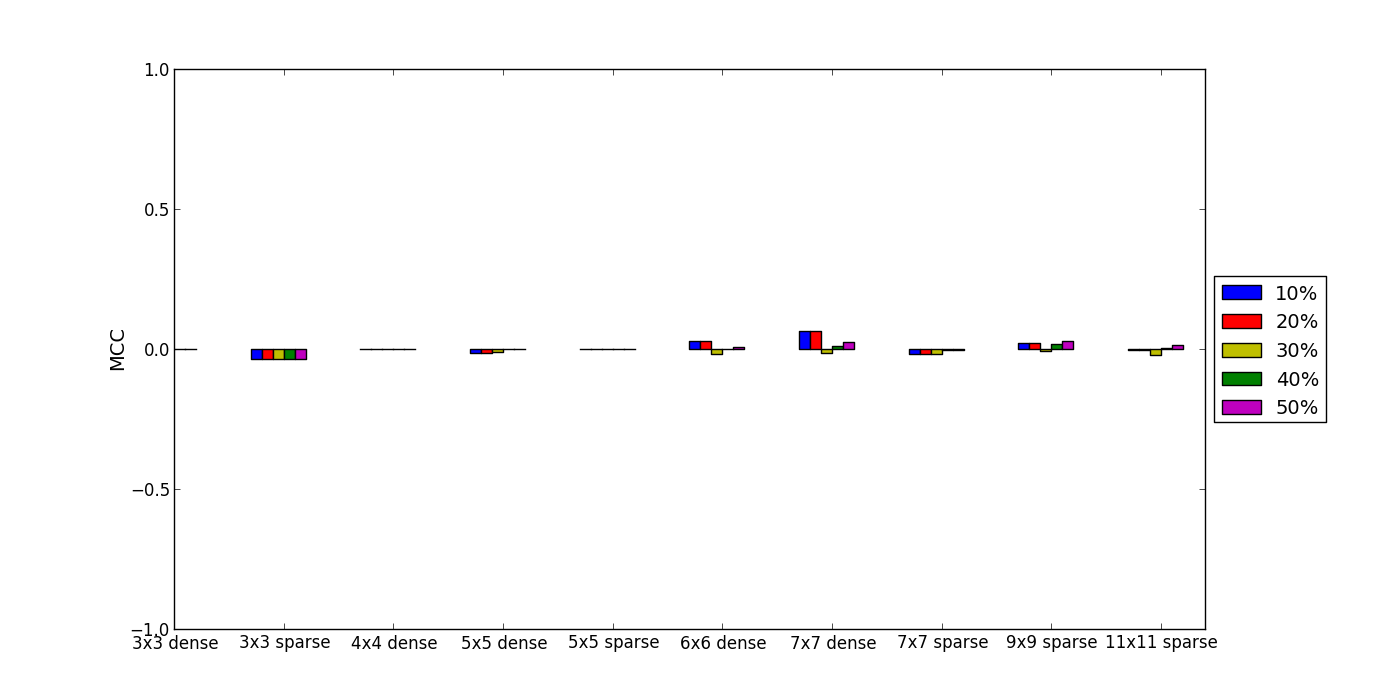
\includegraphics[width=1.2\textwidth]{assets/experiment_charts/time_TextRegion_heading_mcc.png}}
    \caption{TIME: Classificação de títulos}
    \label{fig:time_TextRegion_heading_mcc}
  \end{figure*}

\clearpage

  \subsection{Imagens finais}

    As tabelas \ref{tab:segmentation_689}, \ref{tab:segmentation_692}, \ref{tab:segmentation_695}, \ref{tab:segmentation_802} e \ref{tab:segmentation_803} apresentam as duplas de imagens segmentada e ideal para cada uma das imagens do conjunto de teste CACM. As tabelas \ref{tab:segmentation_783}, \ref{tab:segmentation_784}, \ref{tab:segmentation_785} e\ref{tab:segmentation_786} contém as imagens da TIME. A imagem segmentada exibida foi obtida utilizando o operador morfológico de melhor F-measure (janela 9x9 esparsa com maior número de exemplos de treinamento). A cor azul representa regiões de parágrafo, verde para títulos e vermelho para marcar o que sobrou.

    \begin{table}[p]
      \caption{Segmentação da imagem 689}
      \begin{center}
        \begin{tabular}{ c c }
          Ideal & Segmentada \\
          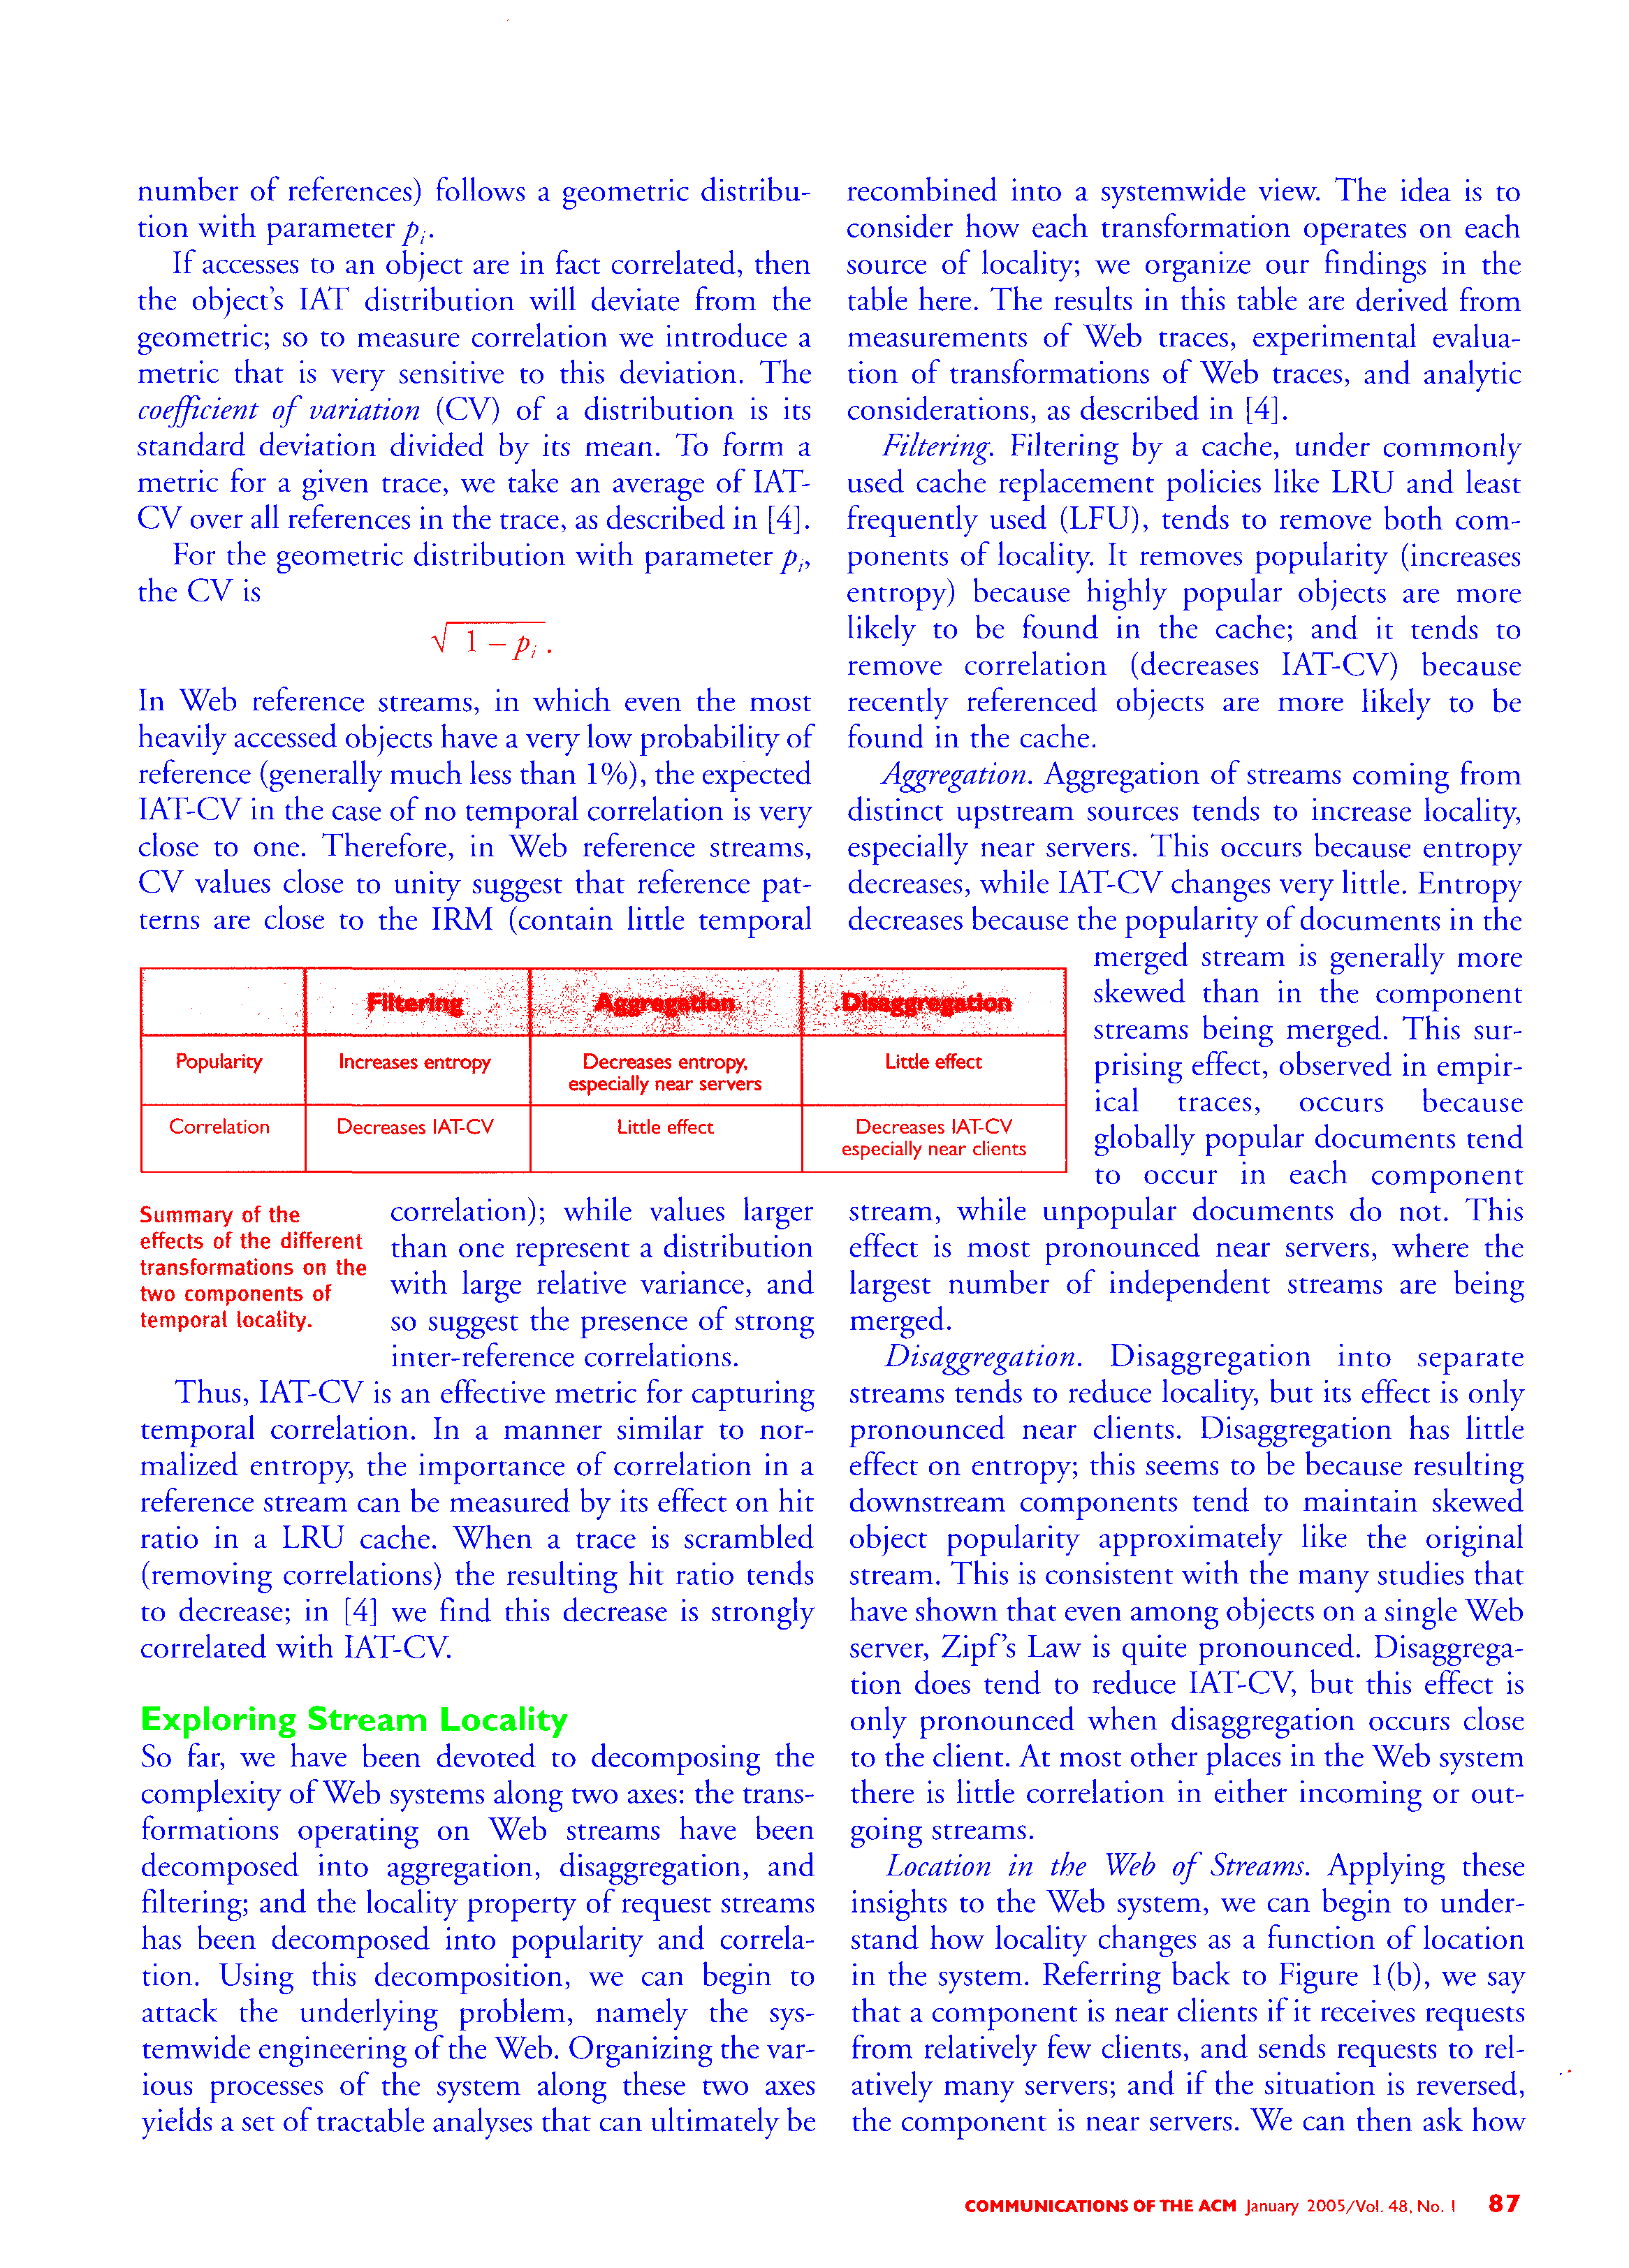
\includegraphics[width=0.4\textwidth]{assets/final_ideal/cacm_689_ideal.png}
          &
          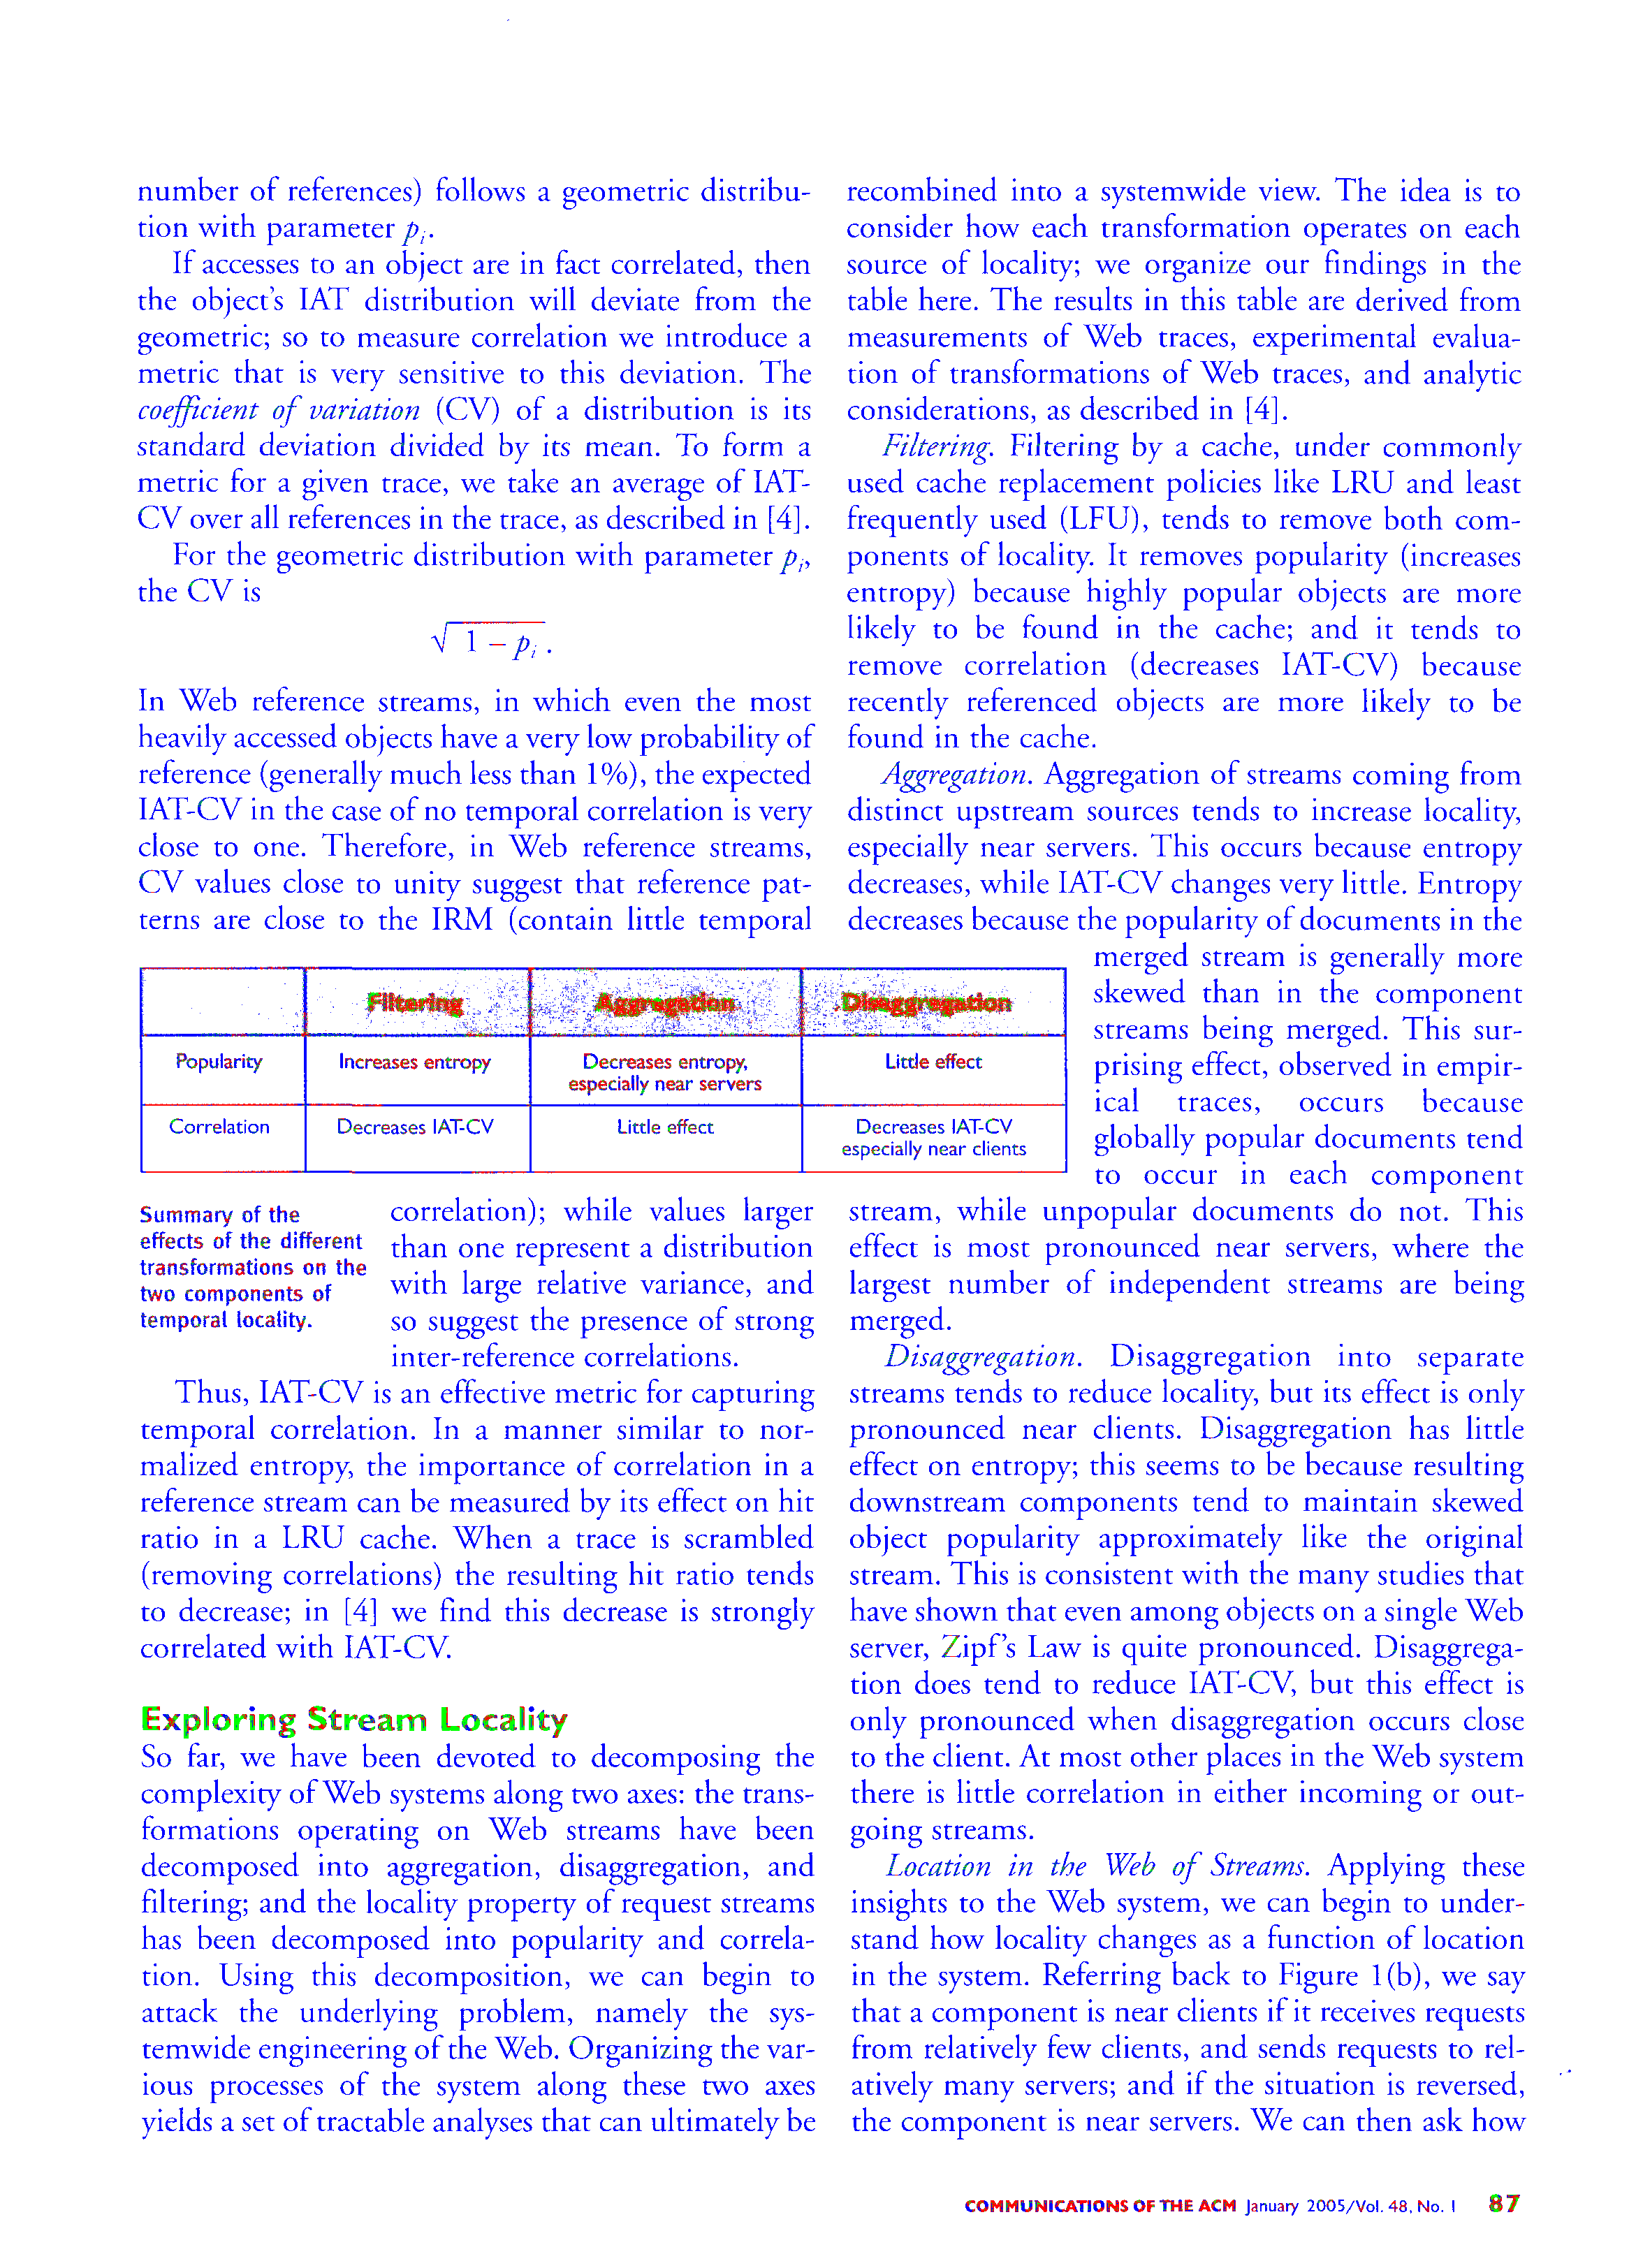
\includegraphics[width=0.4\textwidth]{assets/result_imagens/cacm_50_percent_sparse_9x9_689_final.png}
        \end{tabular}
      \end{center}
      \label{tab:segmentation_689}
    \end{table}
    \begin{table}[p]
      \caption{Segmentação da imagem 692}
      \begin{center}
        \begin{tabular}{ c c }
        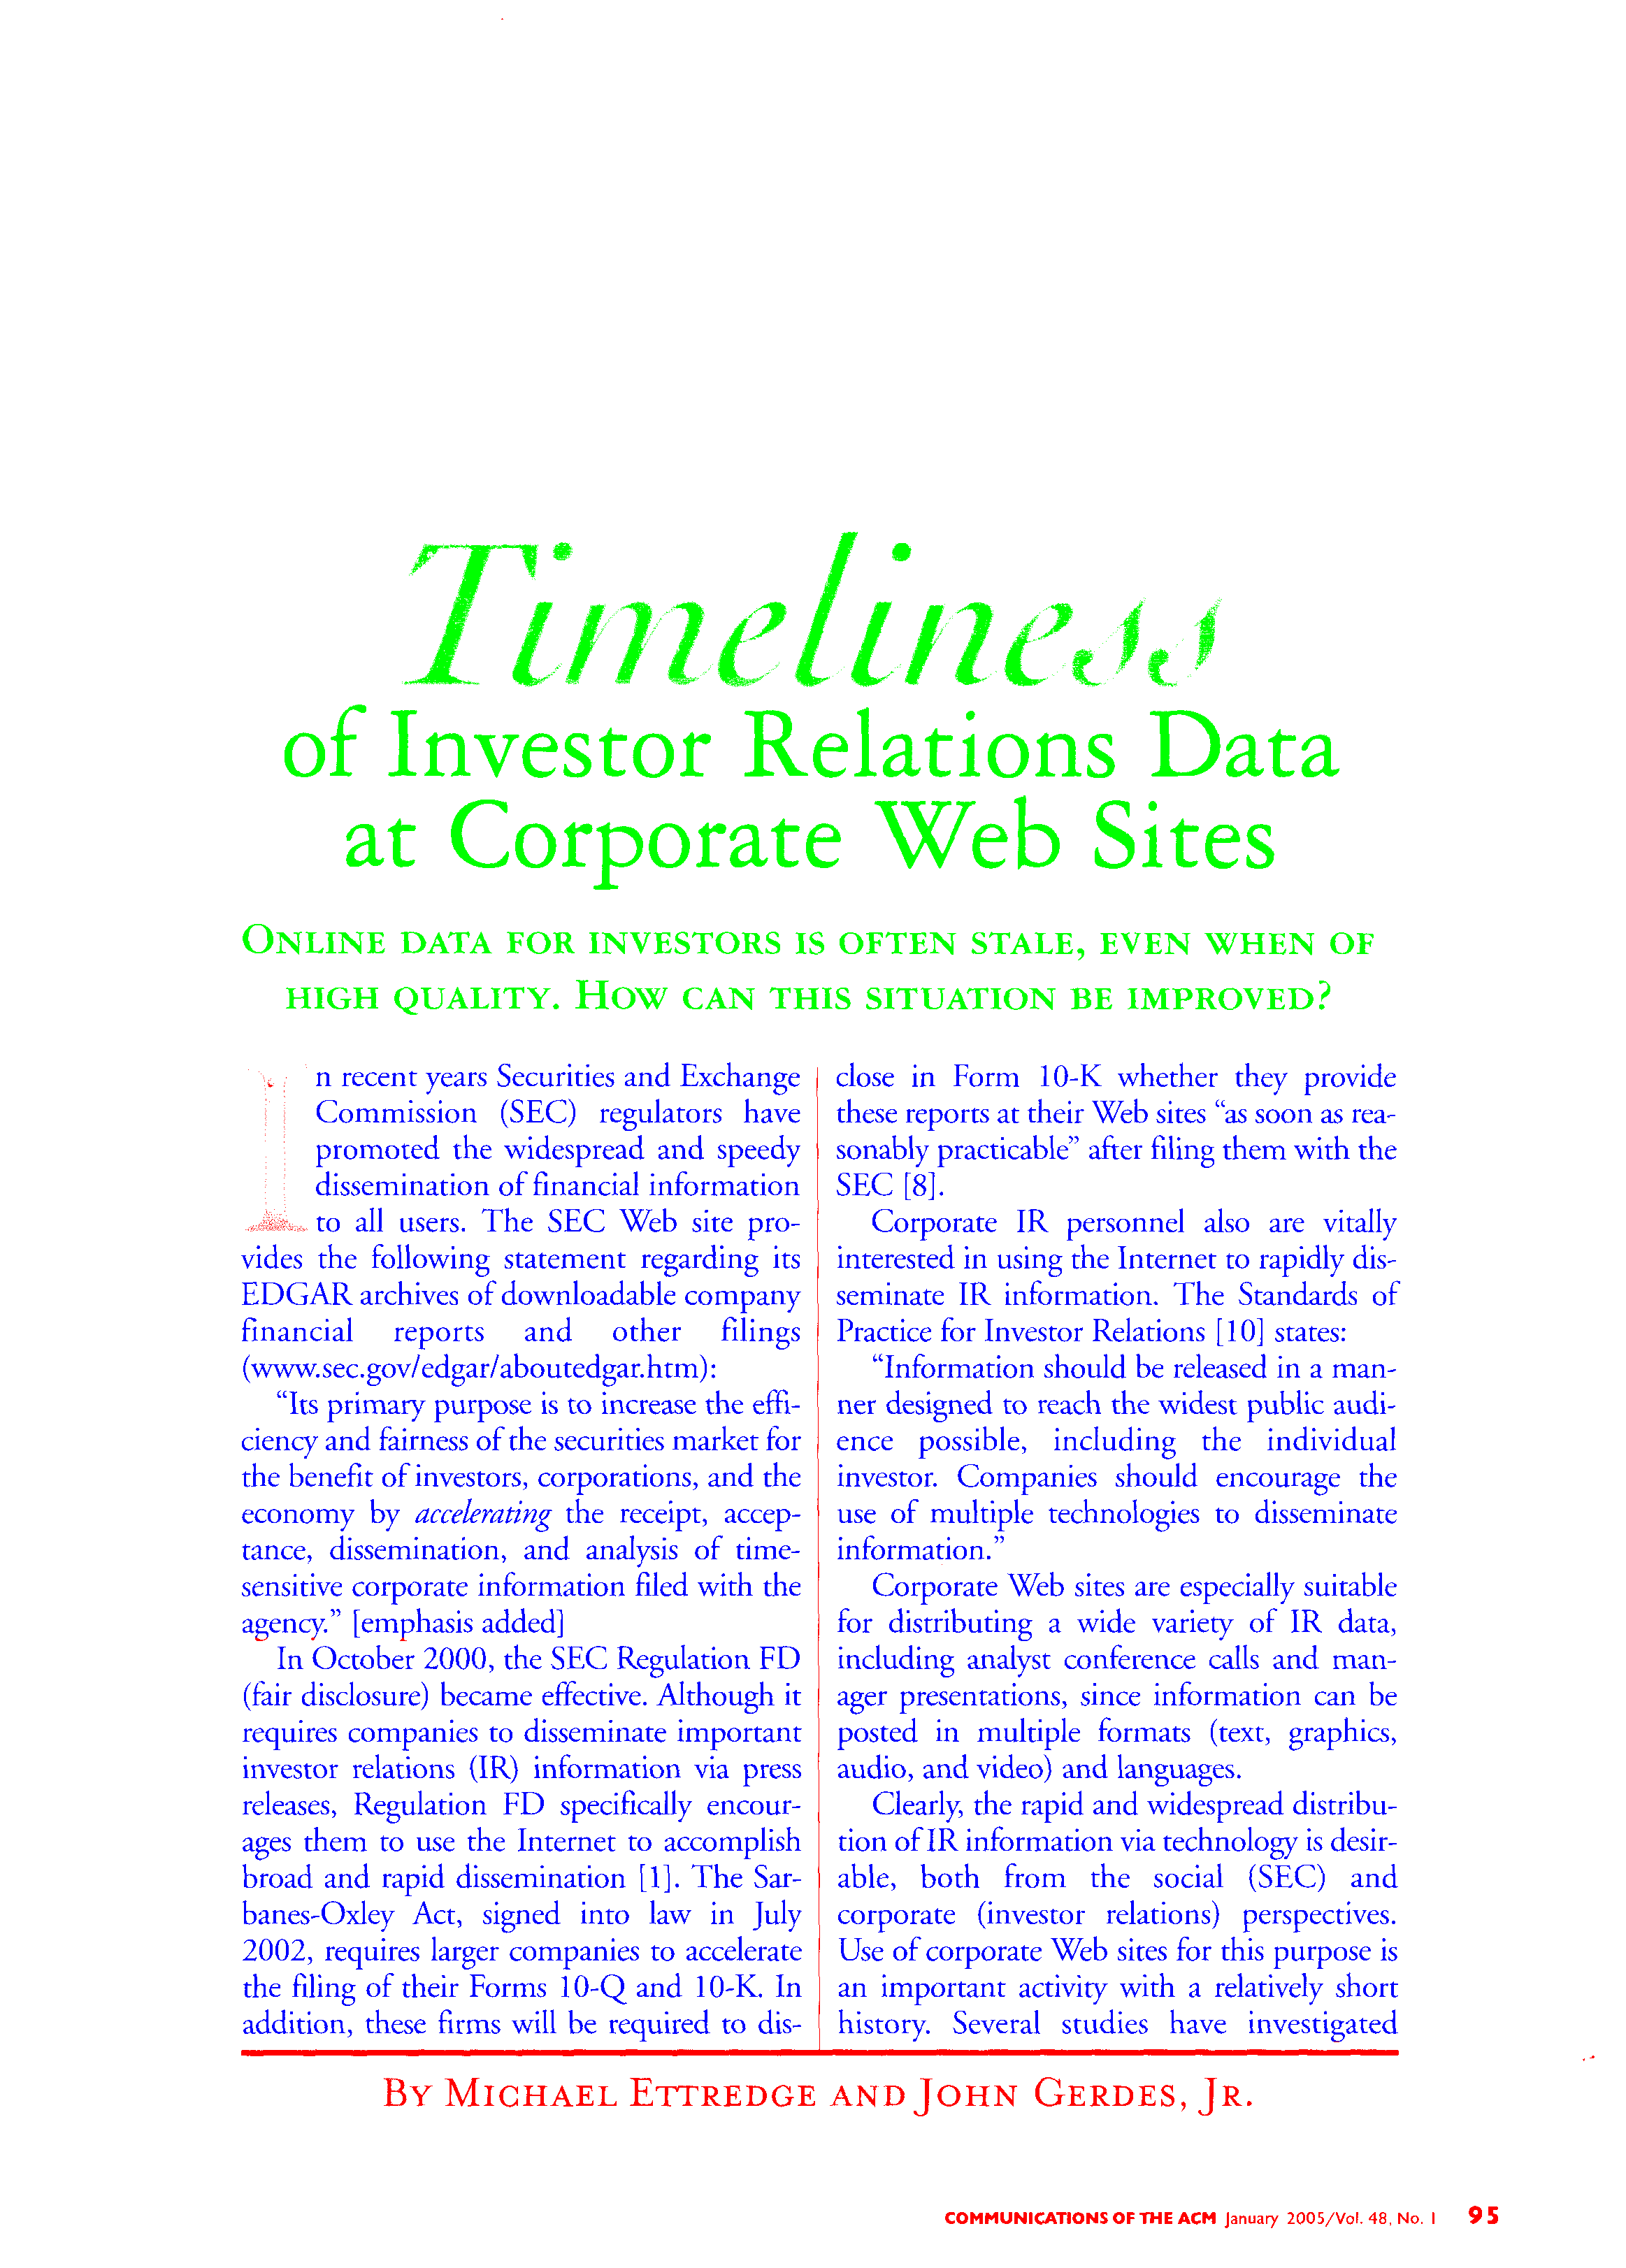
\includegraphics[width=0.4\textwidth]{assets/final_ideal/cacm_692_ideal.png}
        &
        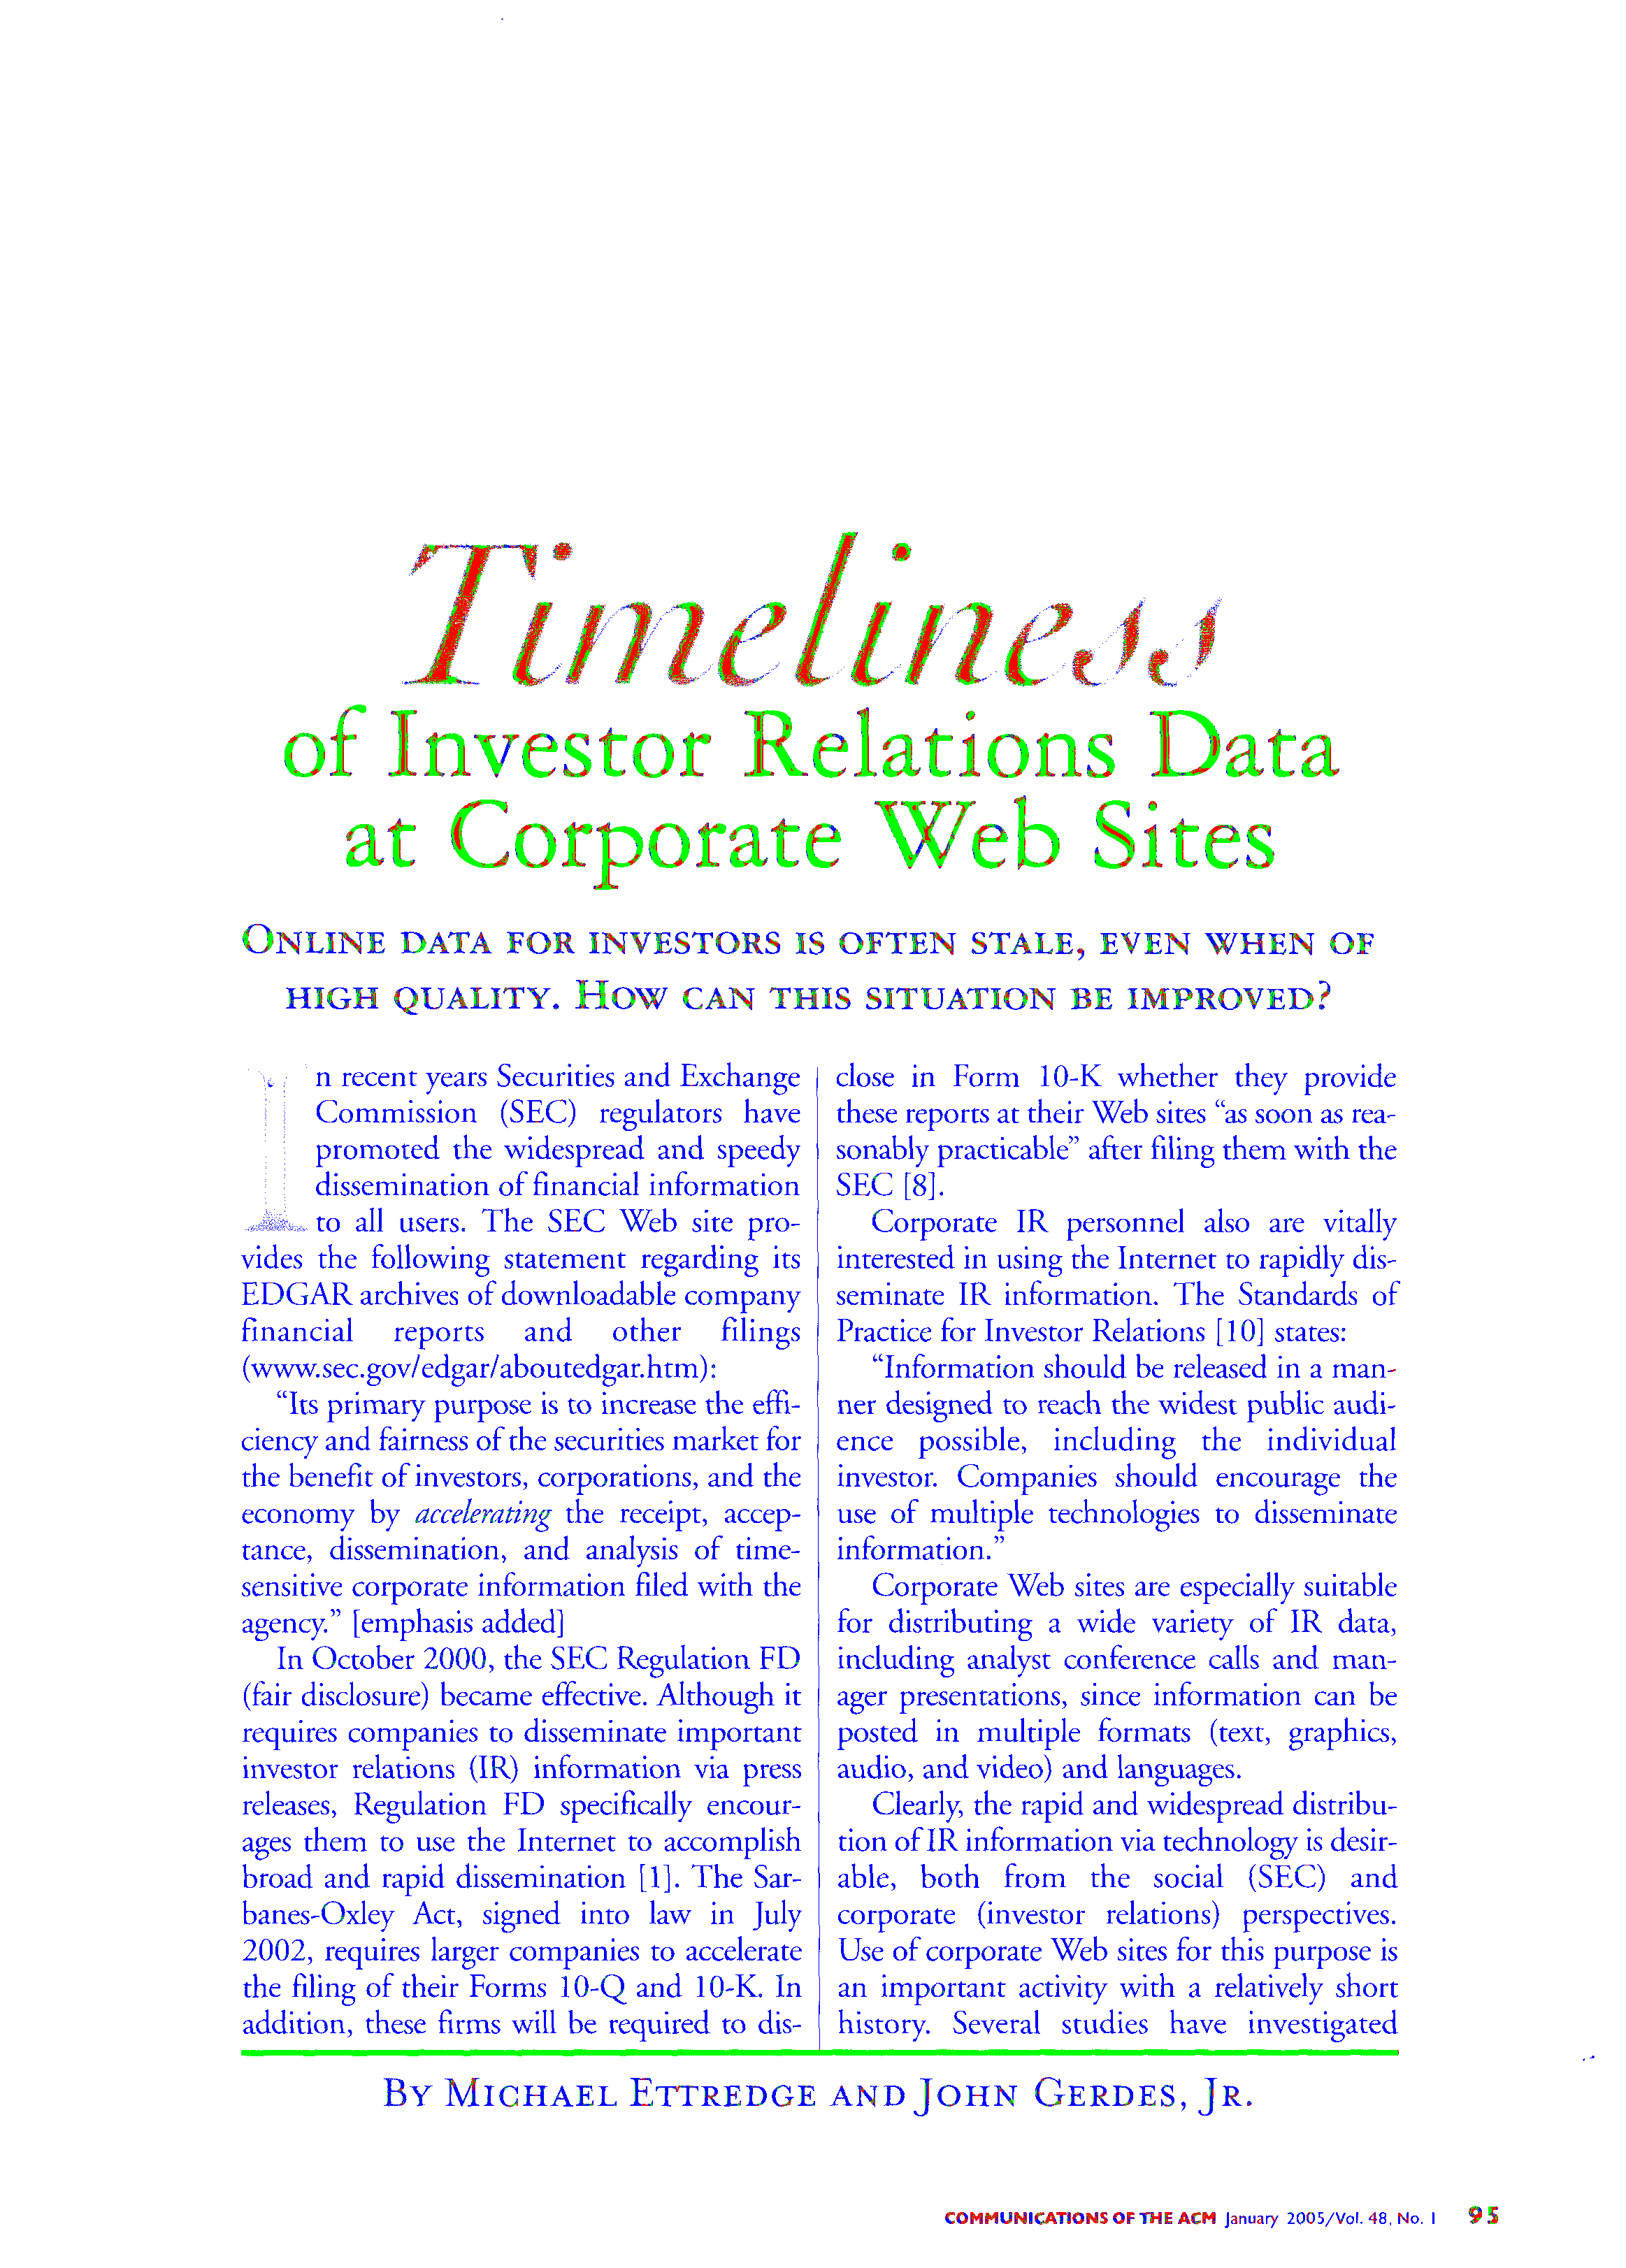
\includegraphics[width=0.4\textwidth]{assets/result_imagens/cacm_50_percent_sparse_9x9_692_final.png}
        \end{tabular}
      \end{center}
      \label{tab:segmentation_692}
    \end{table}
    \begin{table}[p]
      \caption{Segmentação da imagem 695}
      \begin{center}
        \begin{tabular}{ c c }
        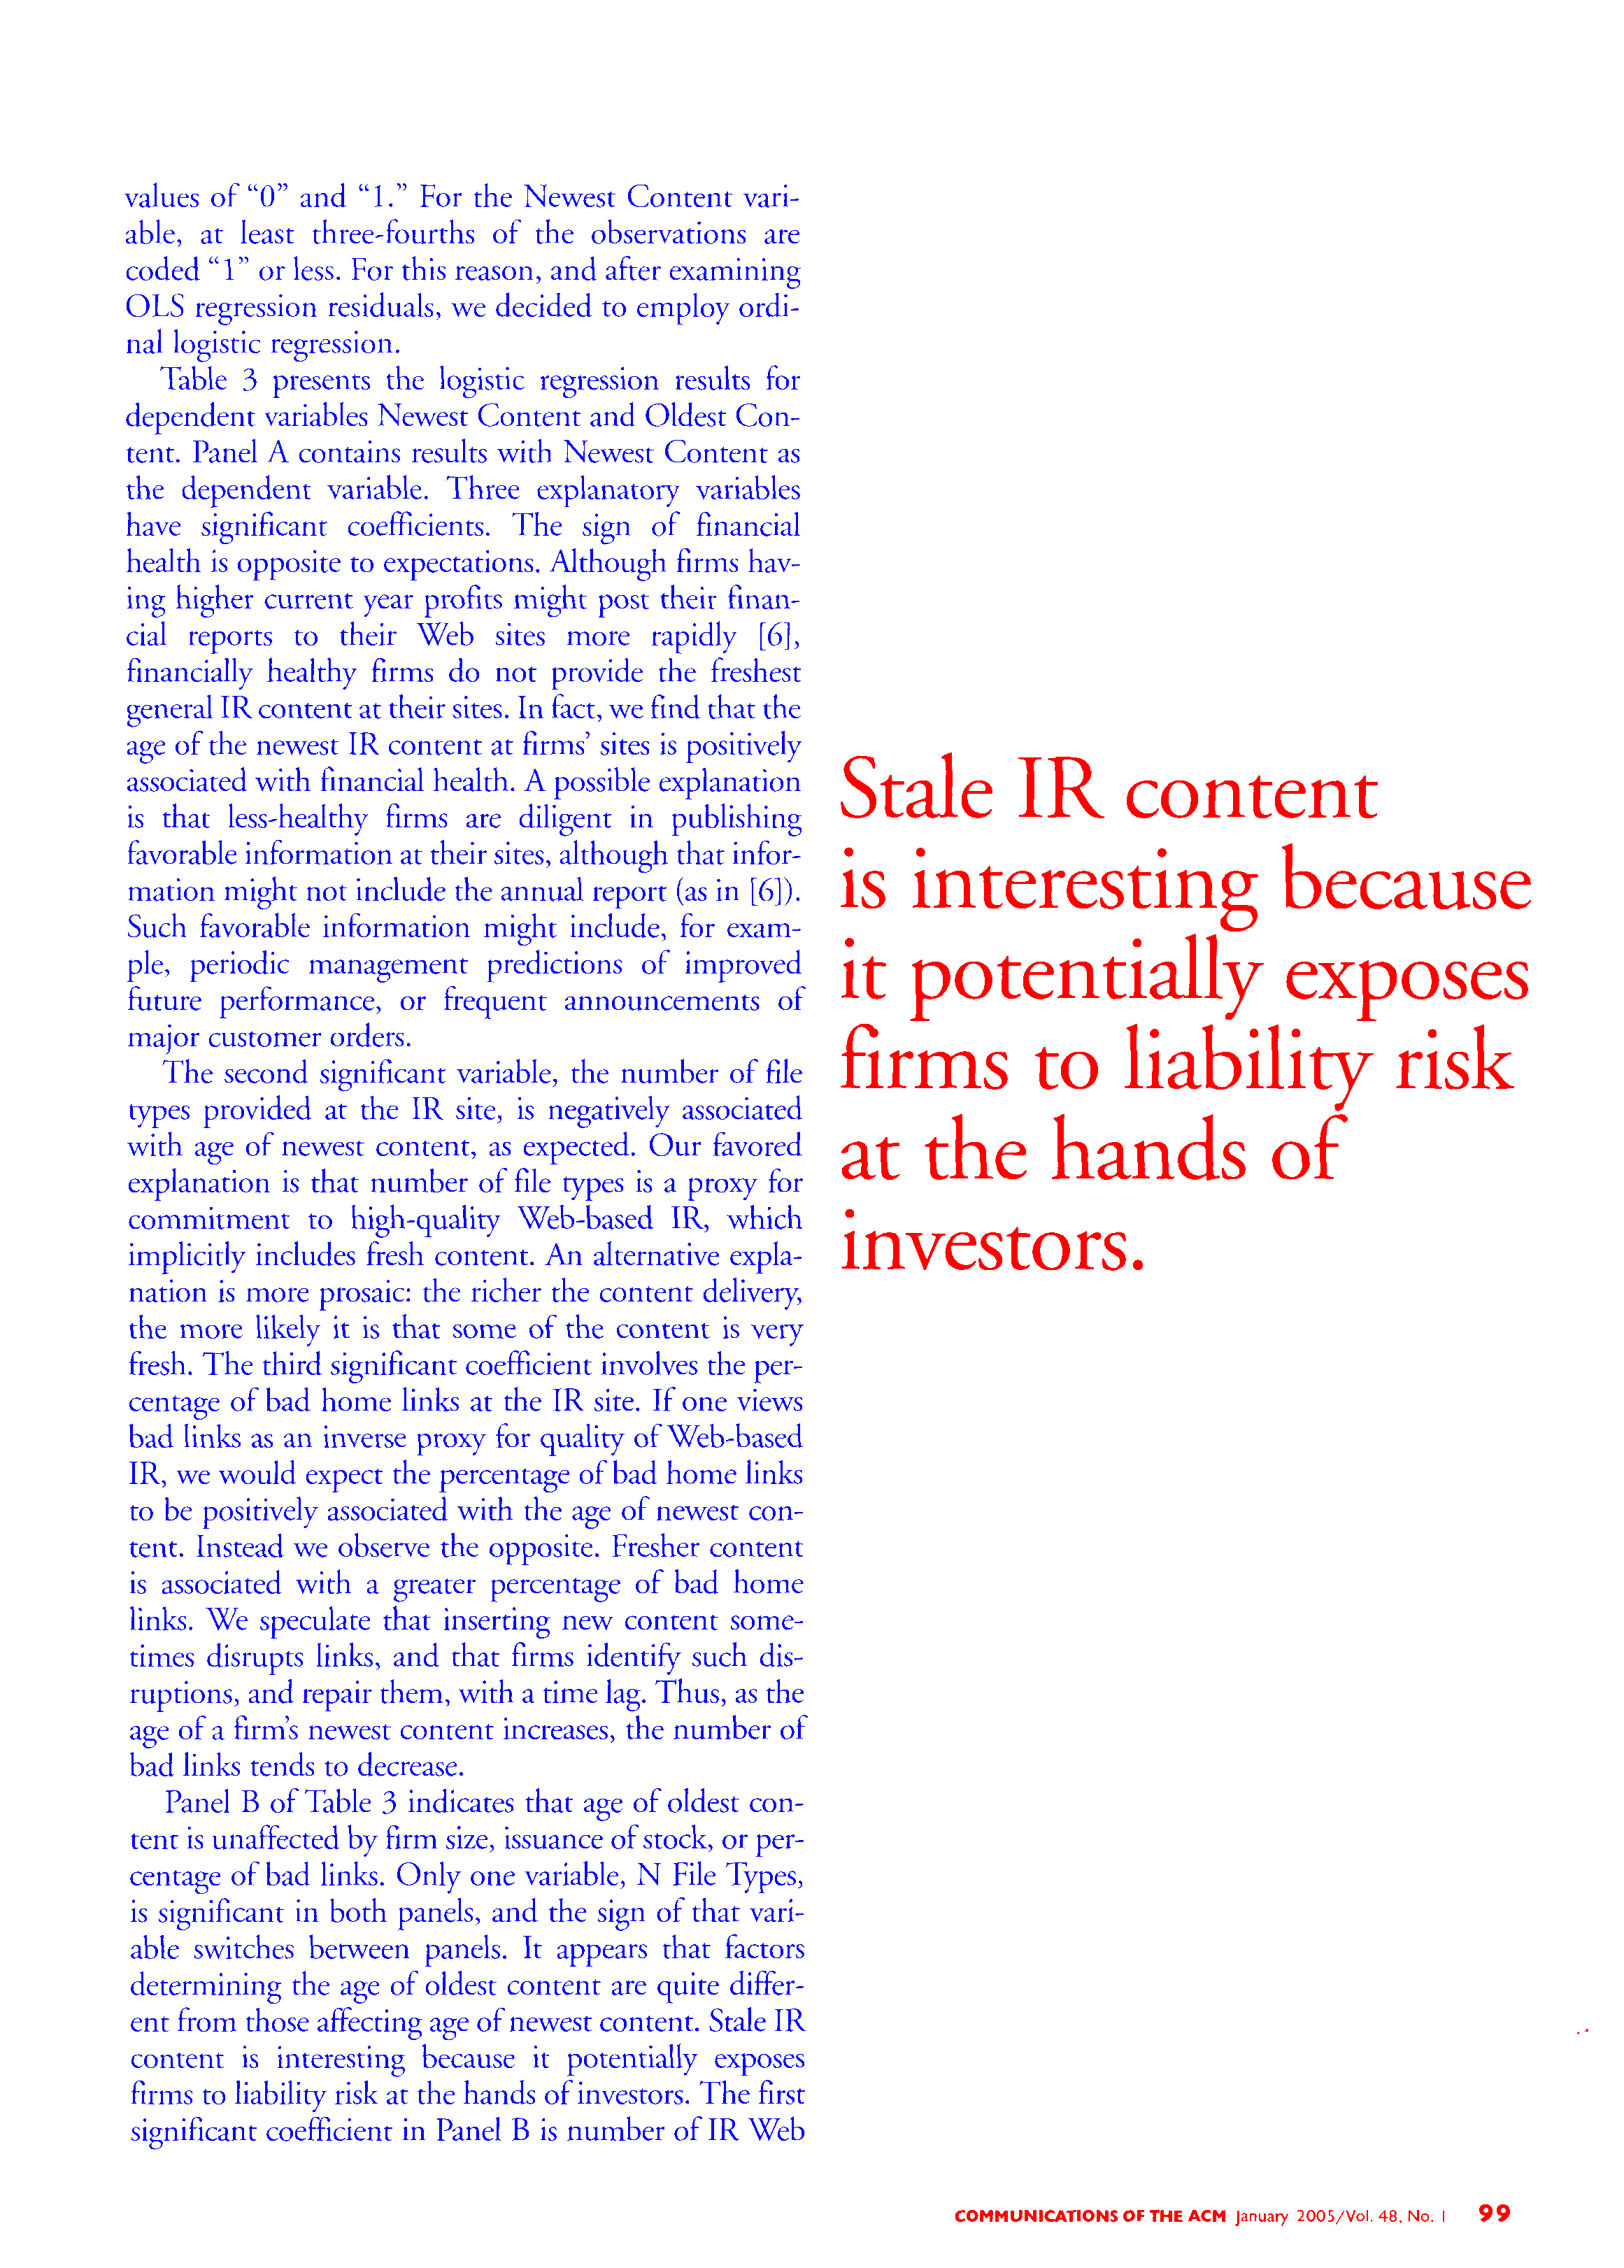
\includegraphics[width=0.4\textwidth]{assets/final_ideal/cacm_695_ideal.png}
        &
        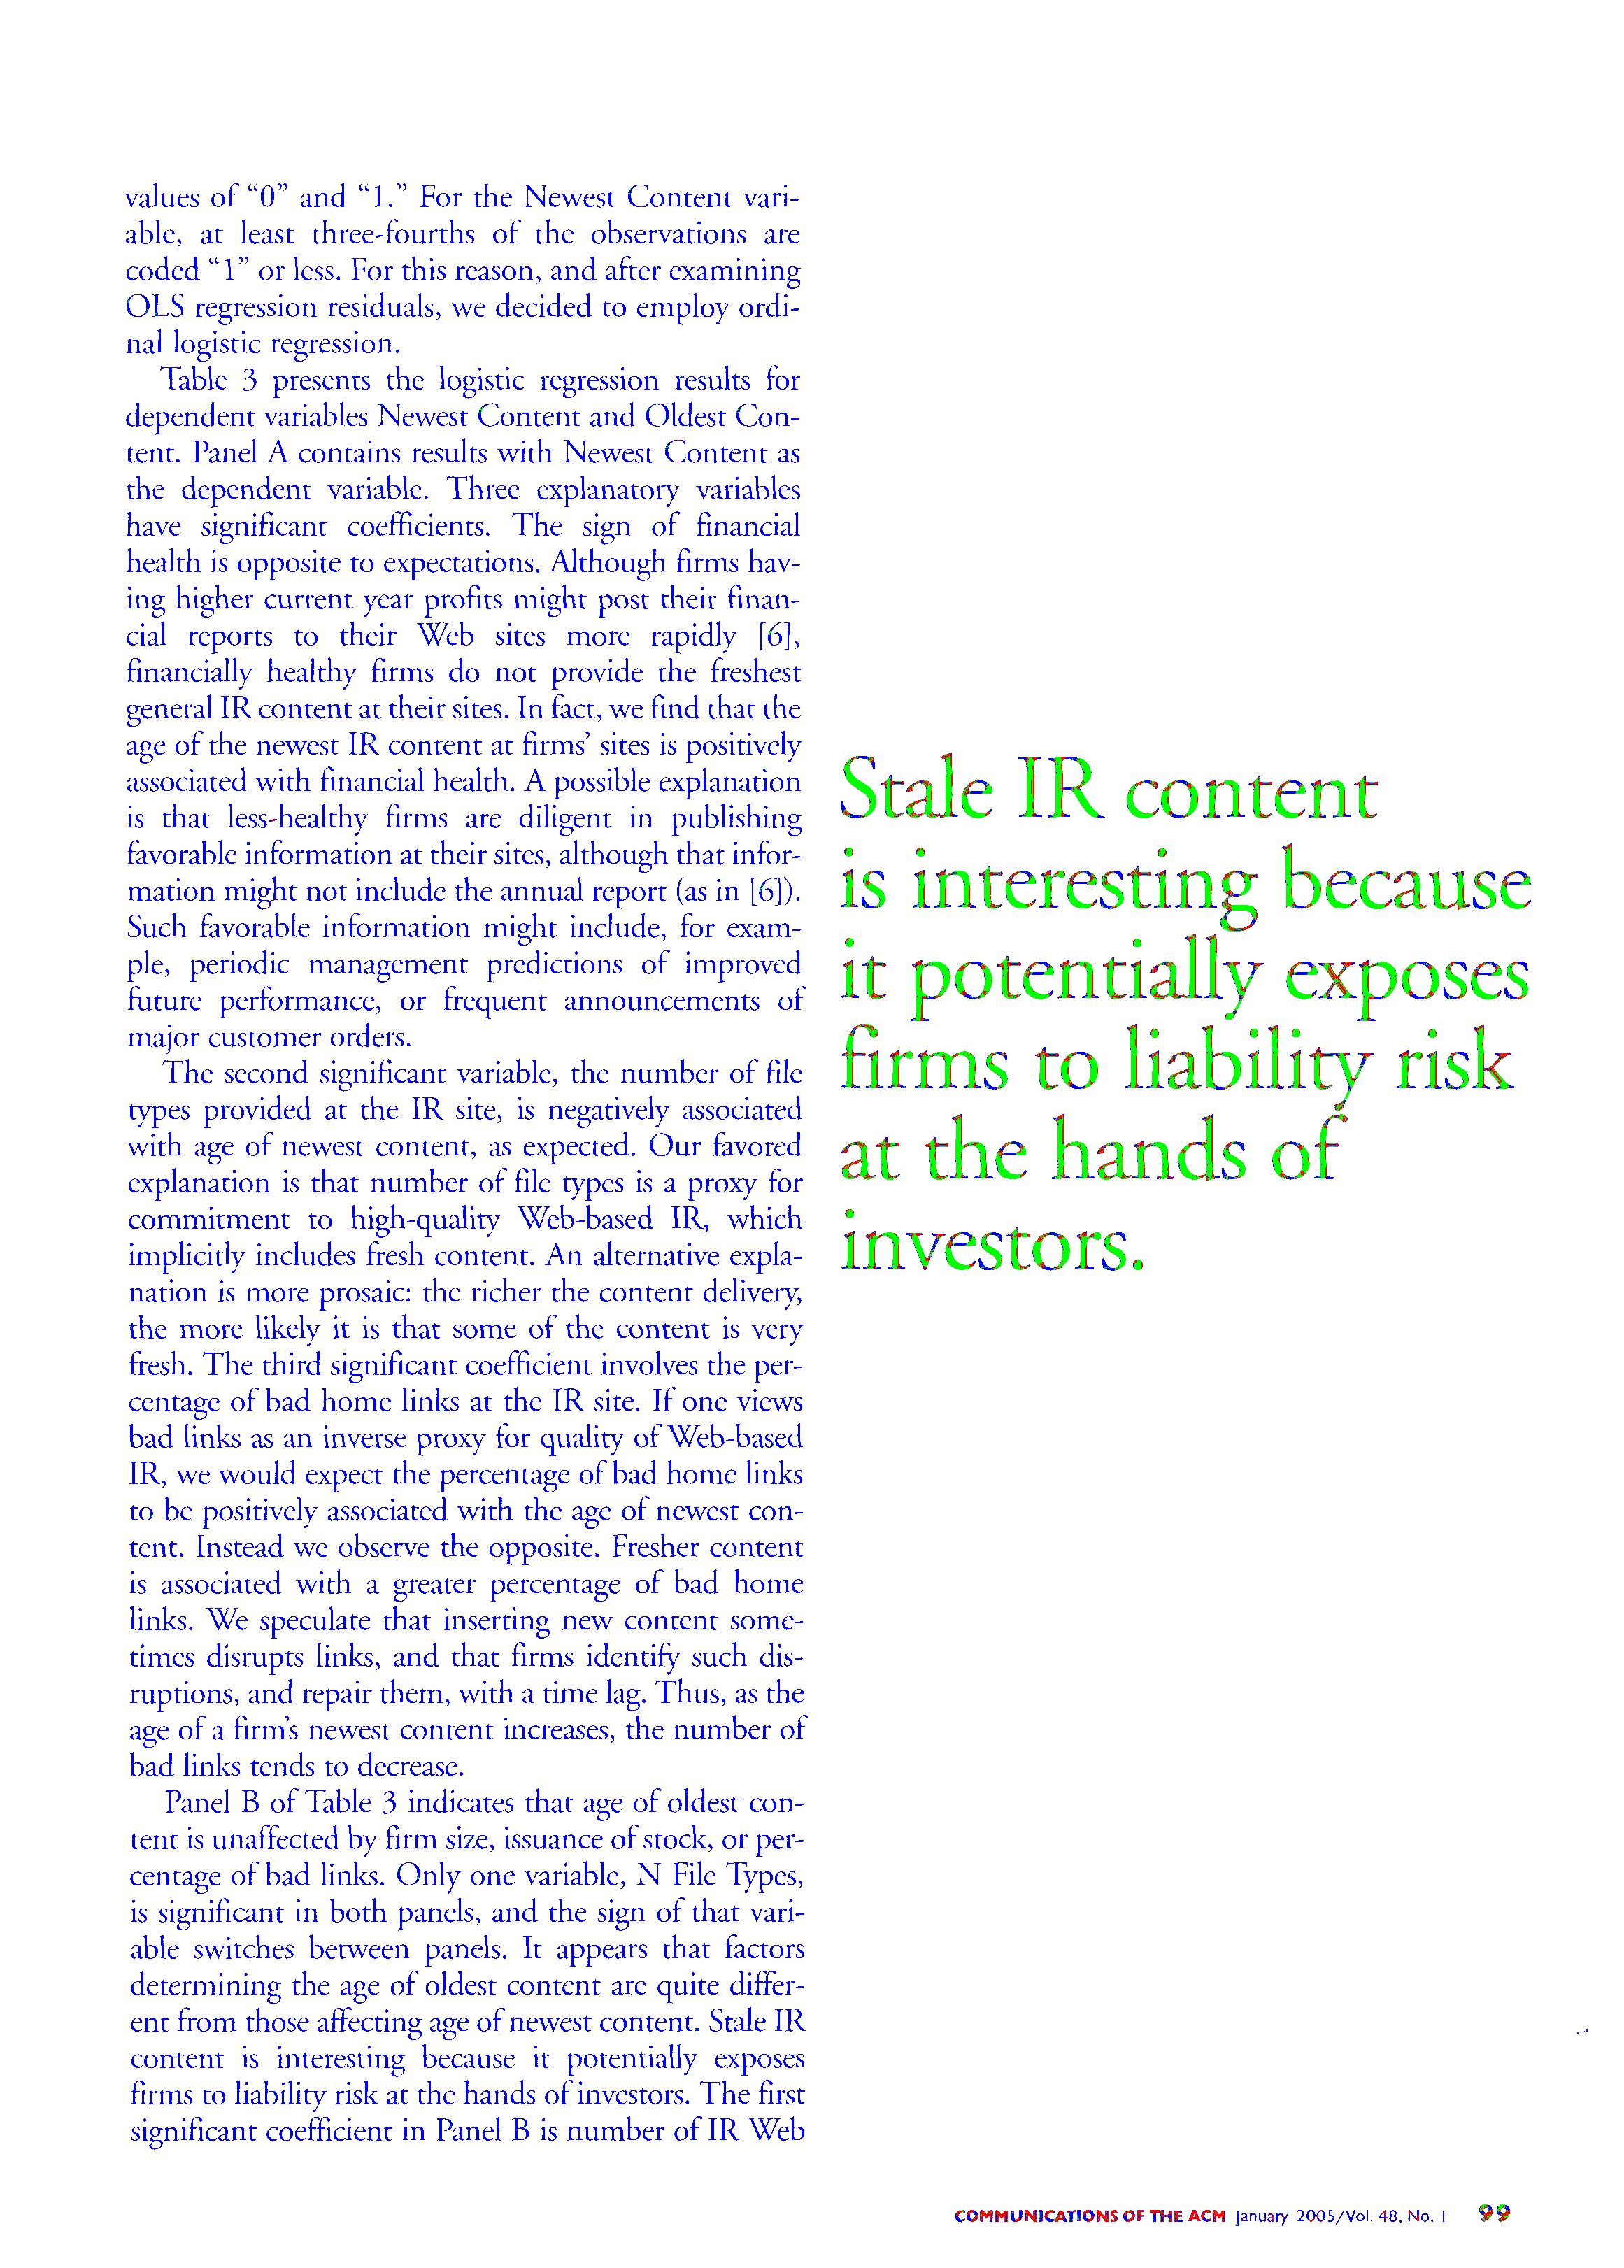
\includegraphics[width=0.4\textwidth]{assets/result_imagens/cacm_50_percent_sparse_9x9_695_final.png}
        \end{tabular}
      \end{center}
      \label{tab:segmentation_695}
    \end{table}
    \begin{table}[p]
      \caption{Segmentação da imagem 802}
      \begin{center}
        \begin{tabular}{ c c }
        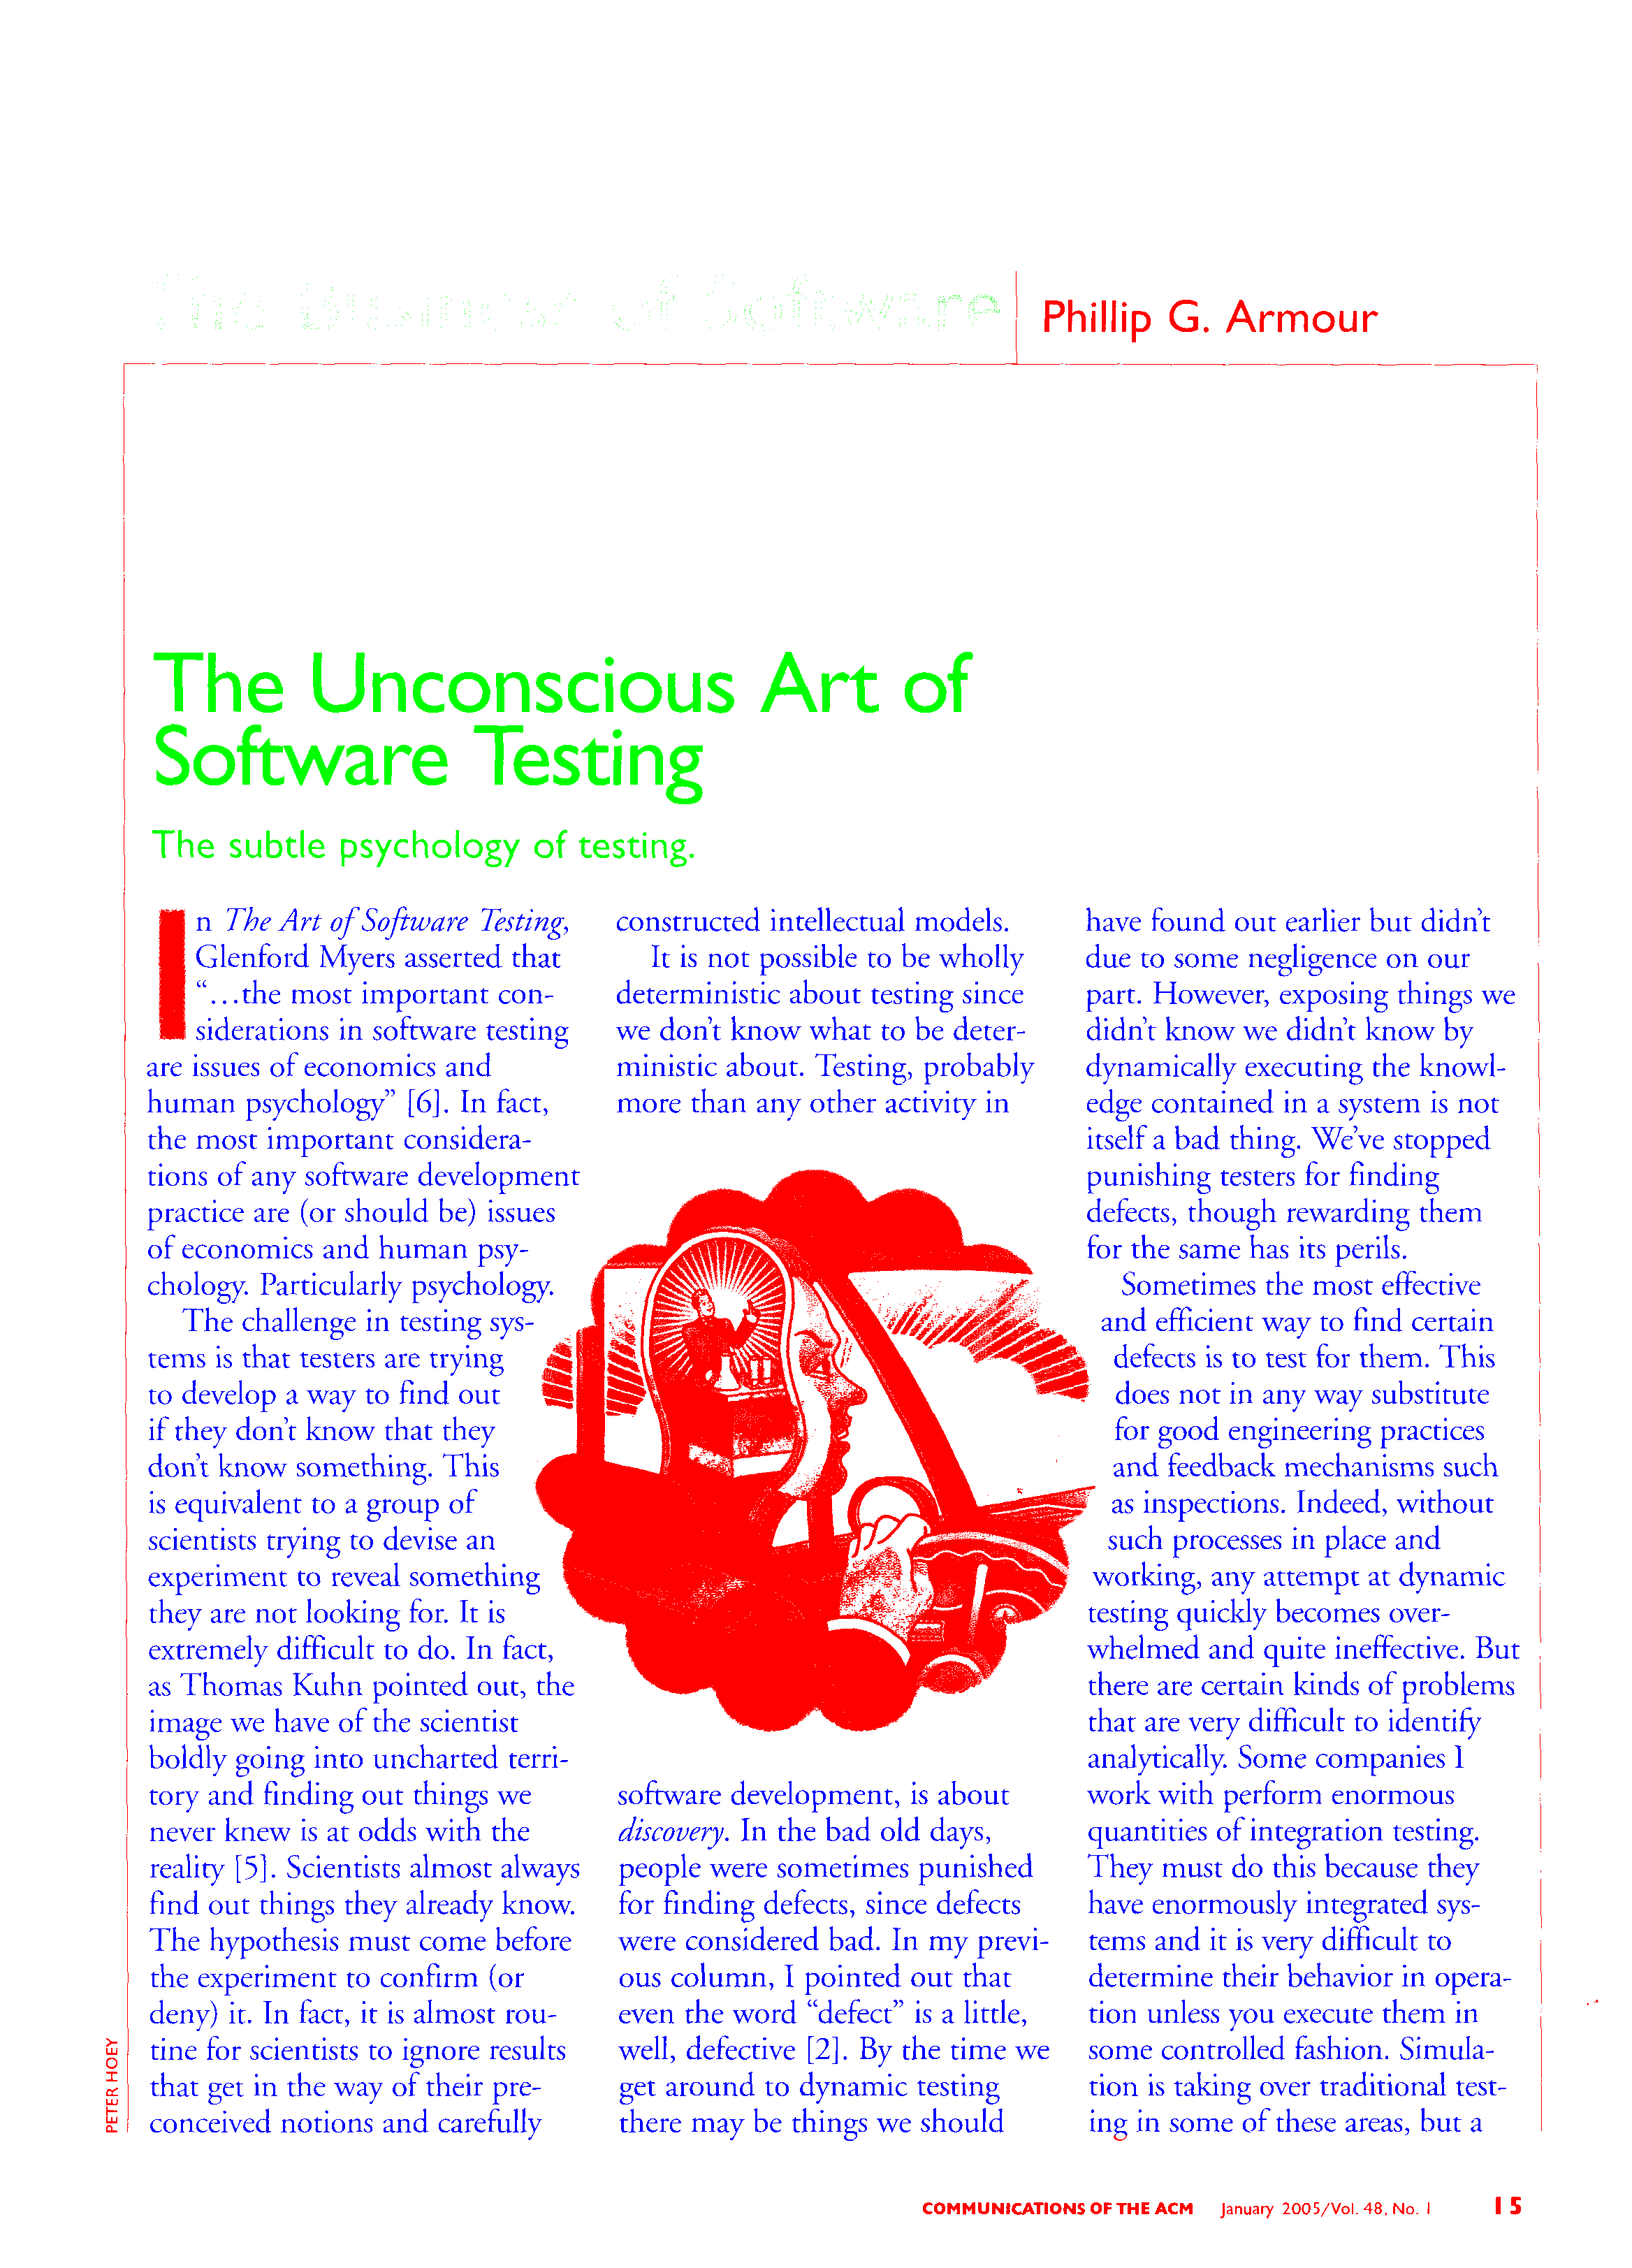
\includegraphics[width=0.4\textwidth]{assets/final_ideal/cacm_802_ideal.png}
        &
        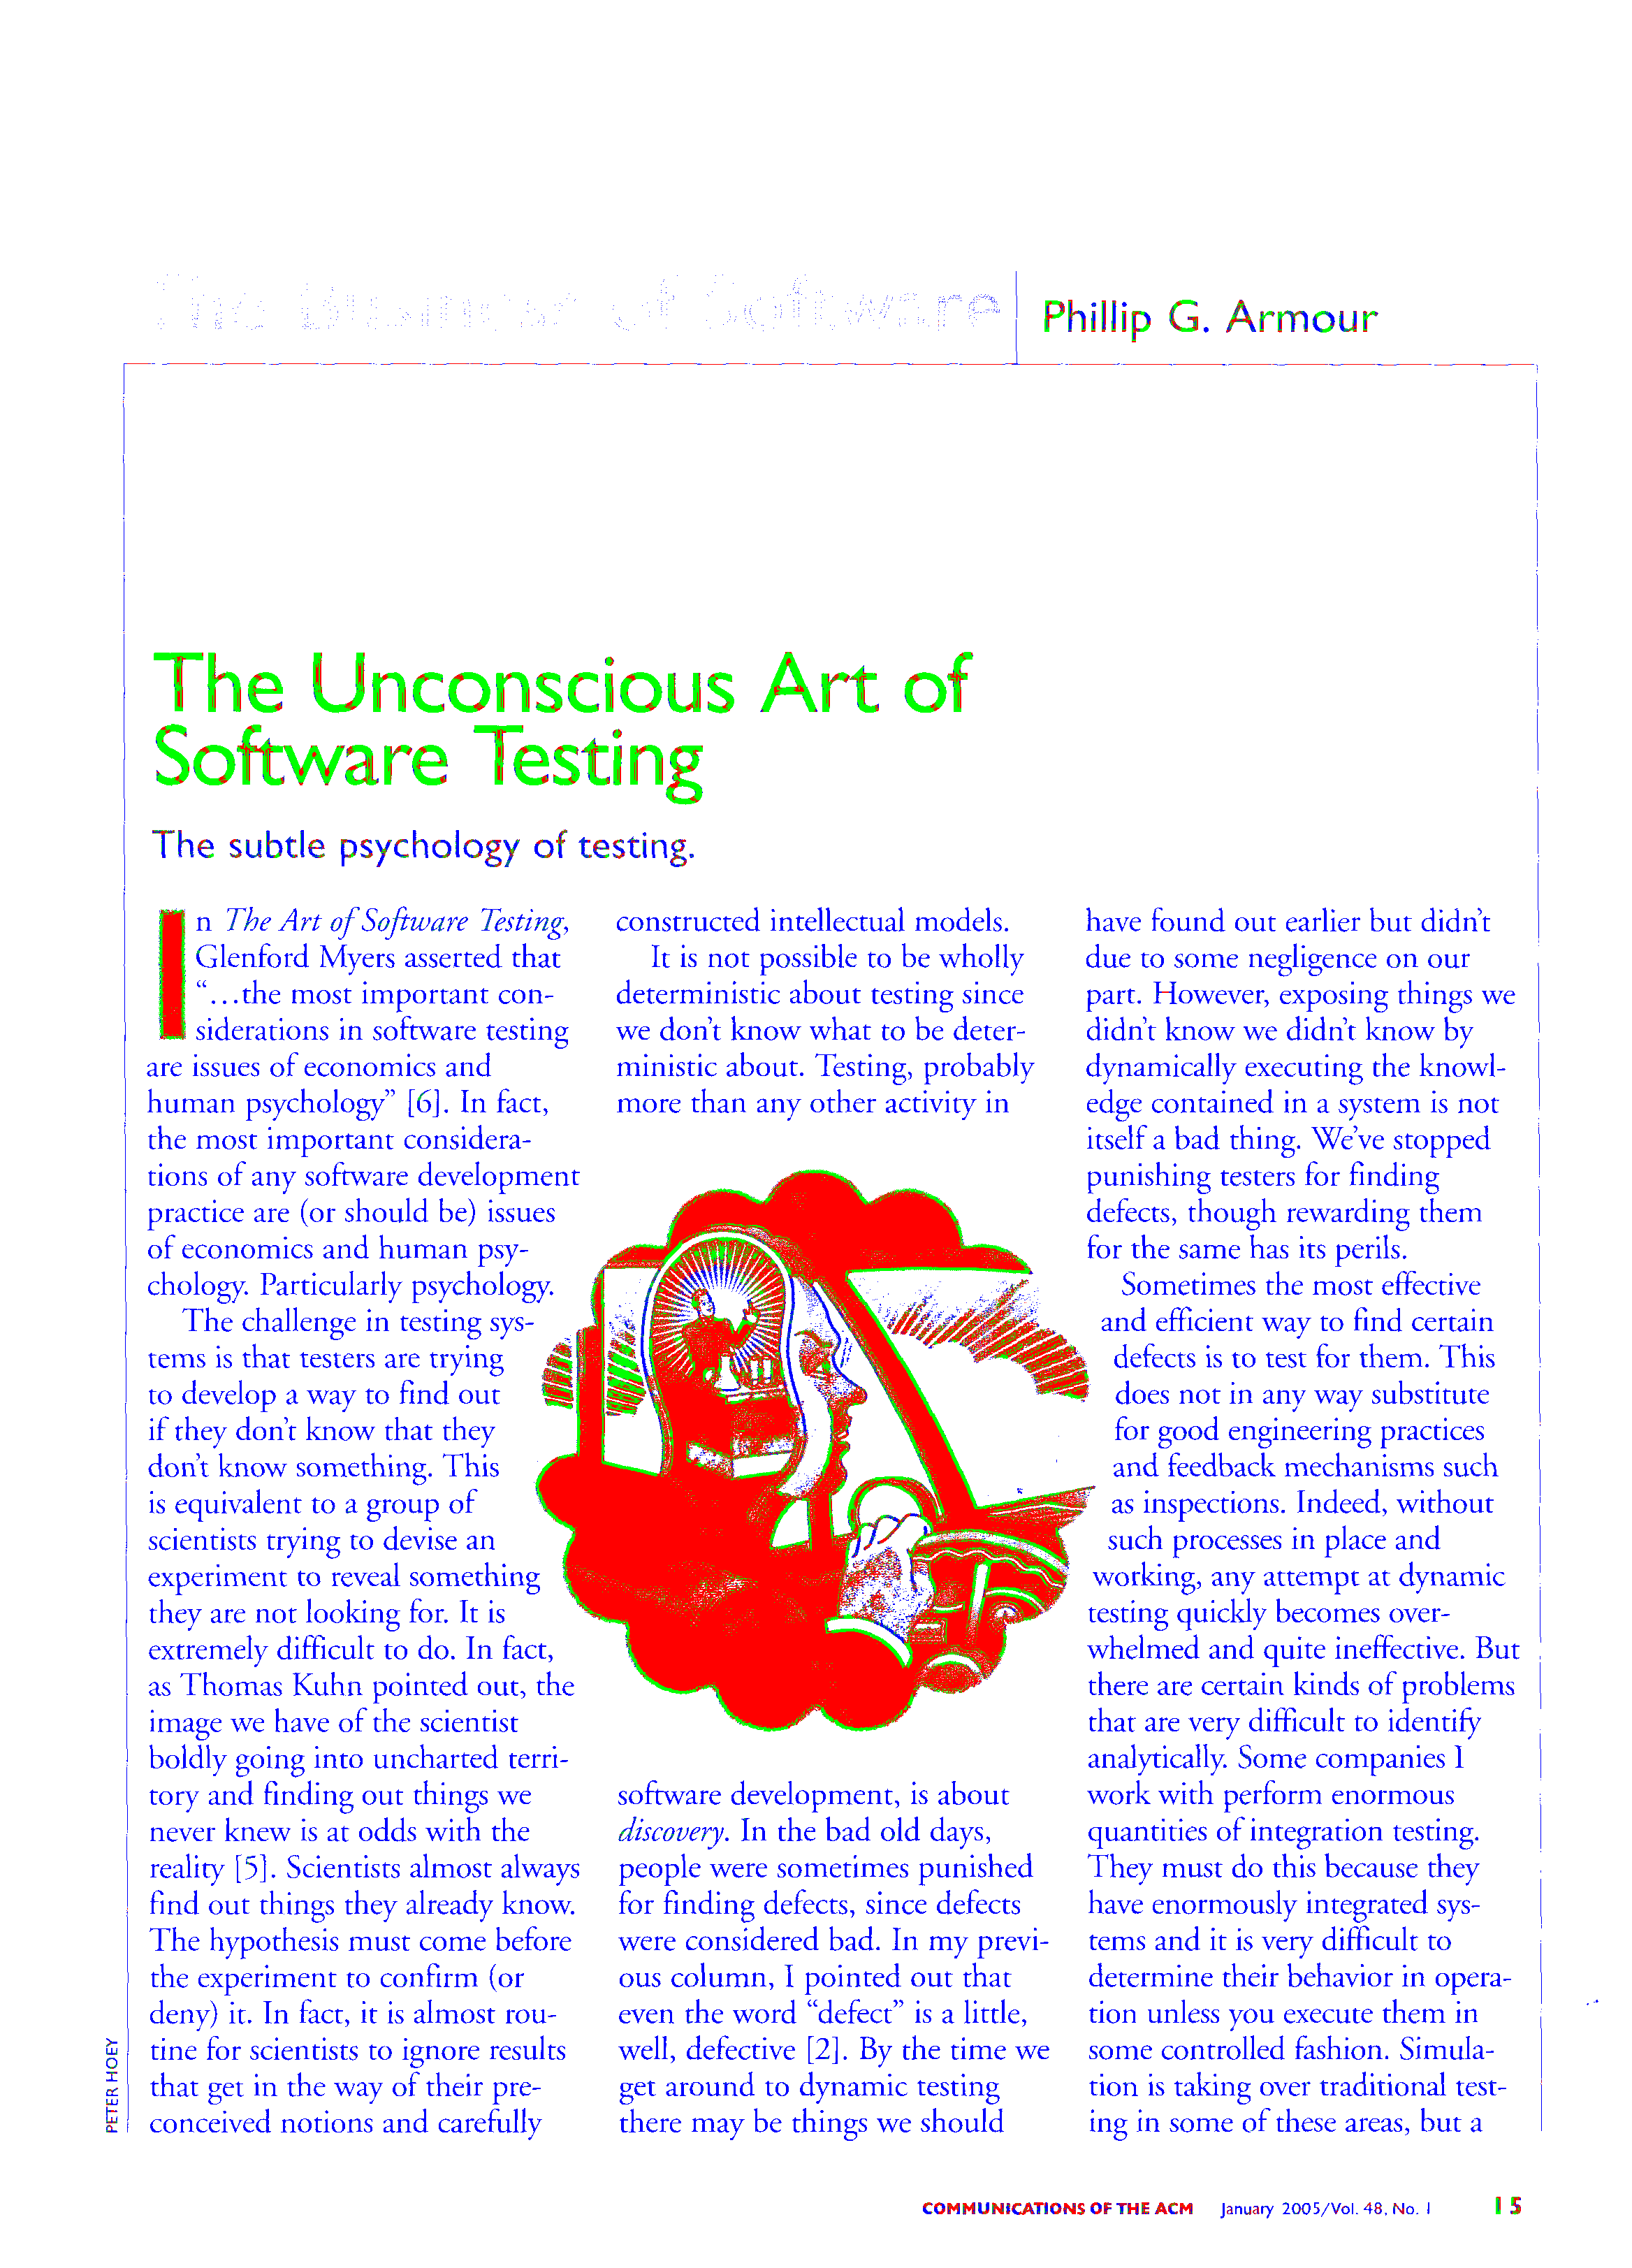
\includegraphics[width=0.4\textwidth]{assets/result_imagens/cacm_50_percent_sparse_9x9_802_final.png}
        \end{tabular}
      \end{center}
      \label{tab:segmentation_802}
    \end{table}
    \begin{table}[p]
      \caption{Segmentação da imagem 803}
      \begin{center}
        \begin{tabular}{ c c }
        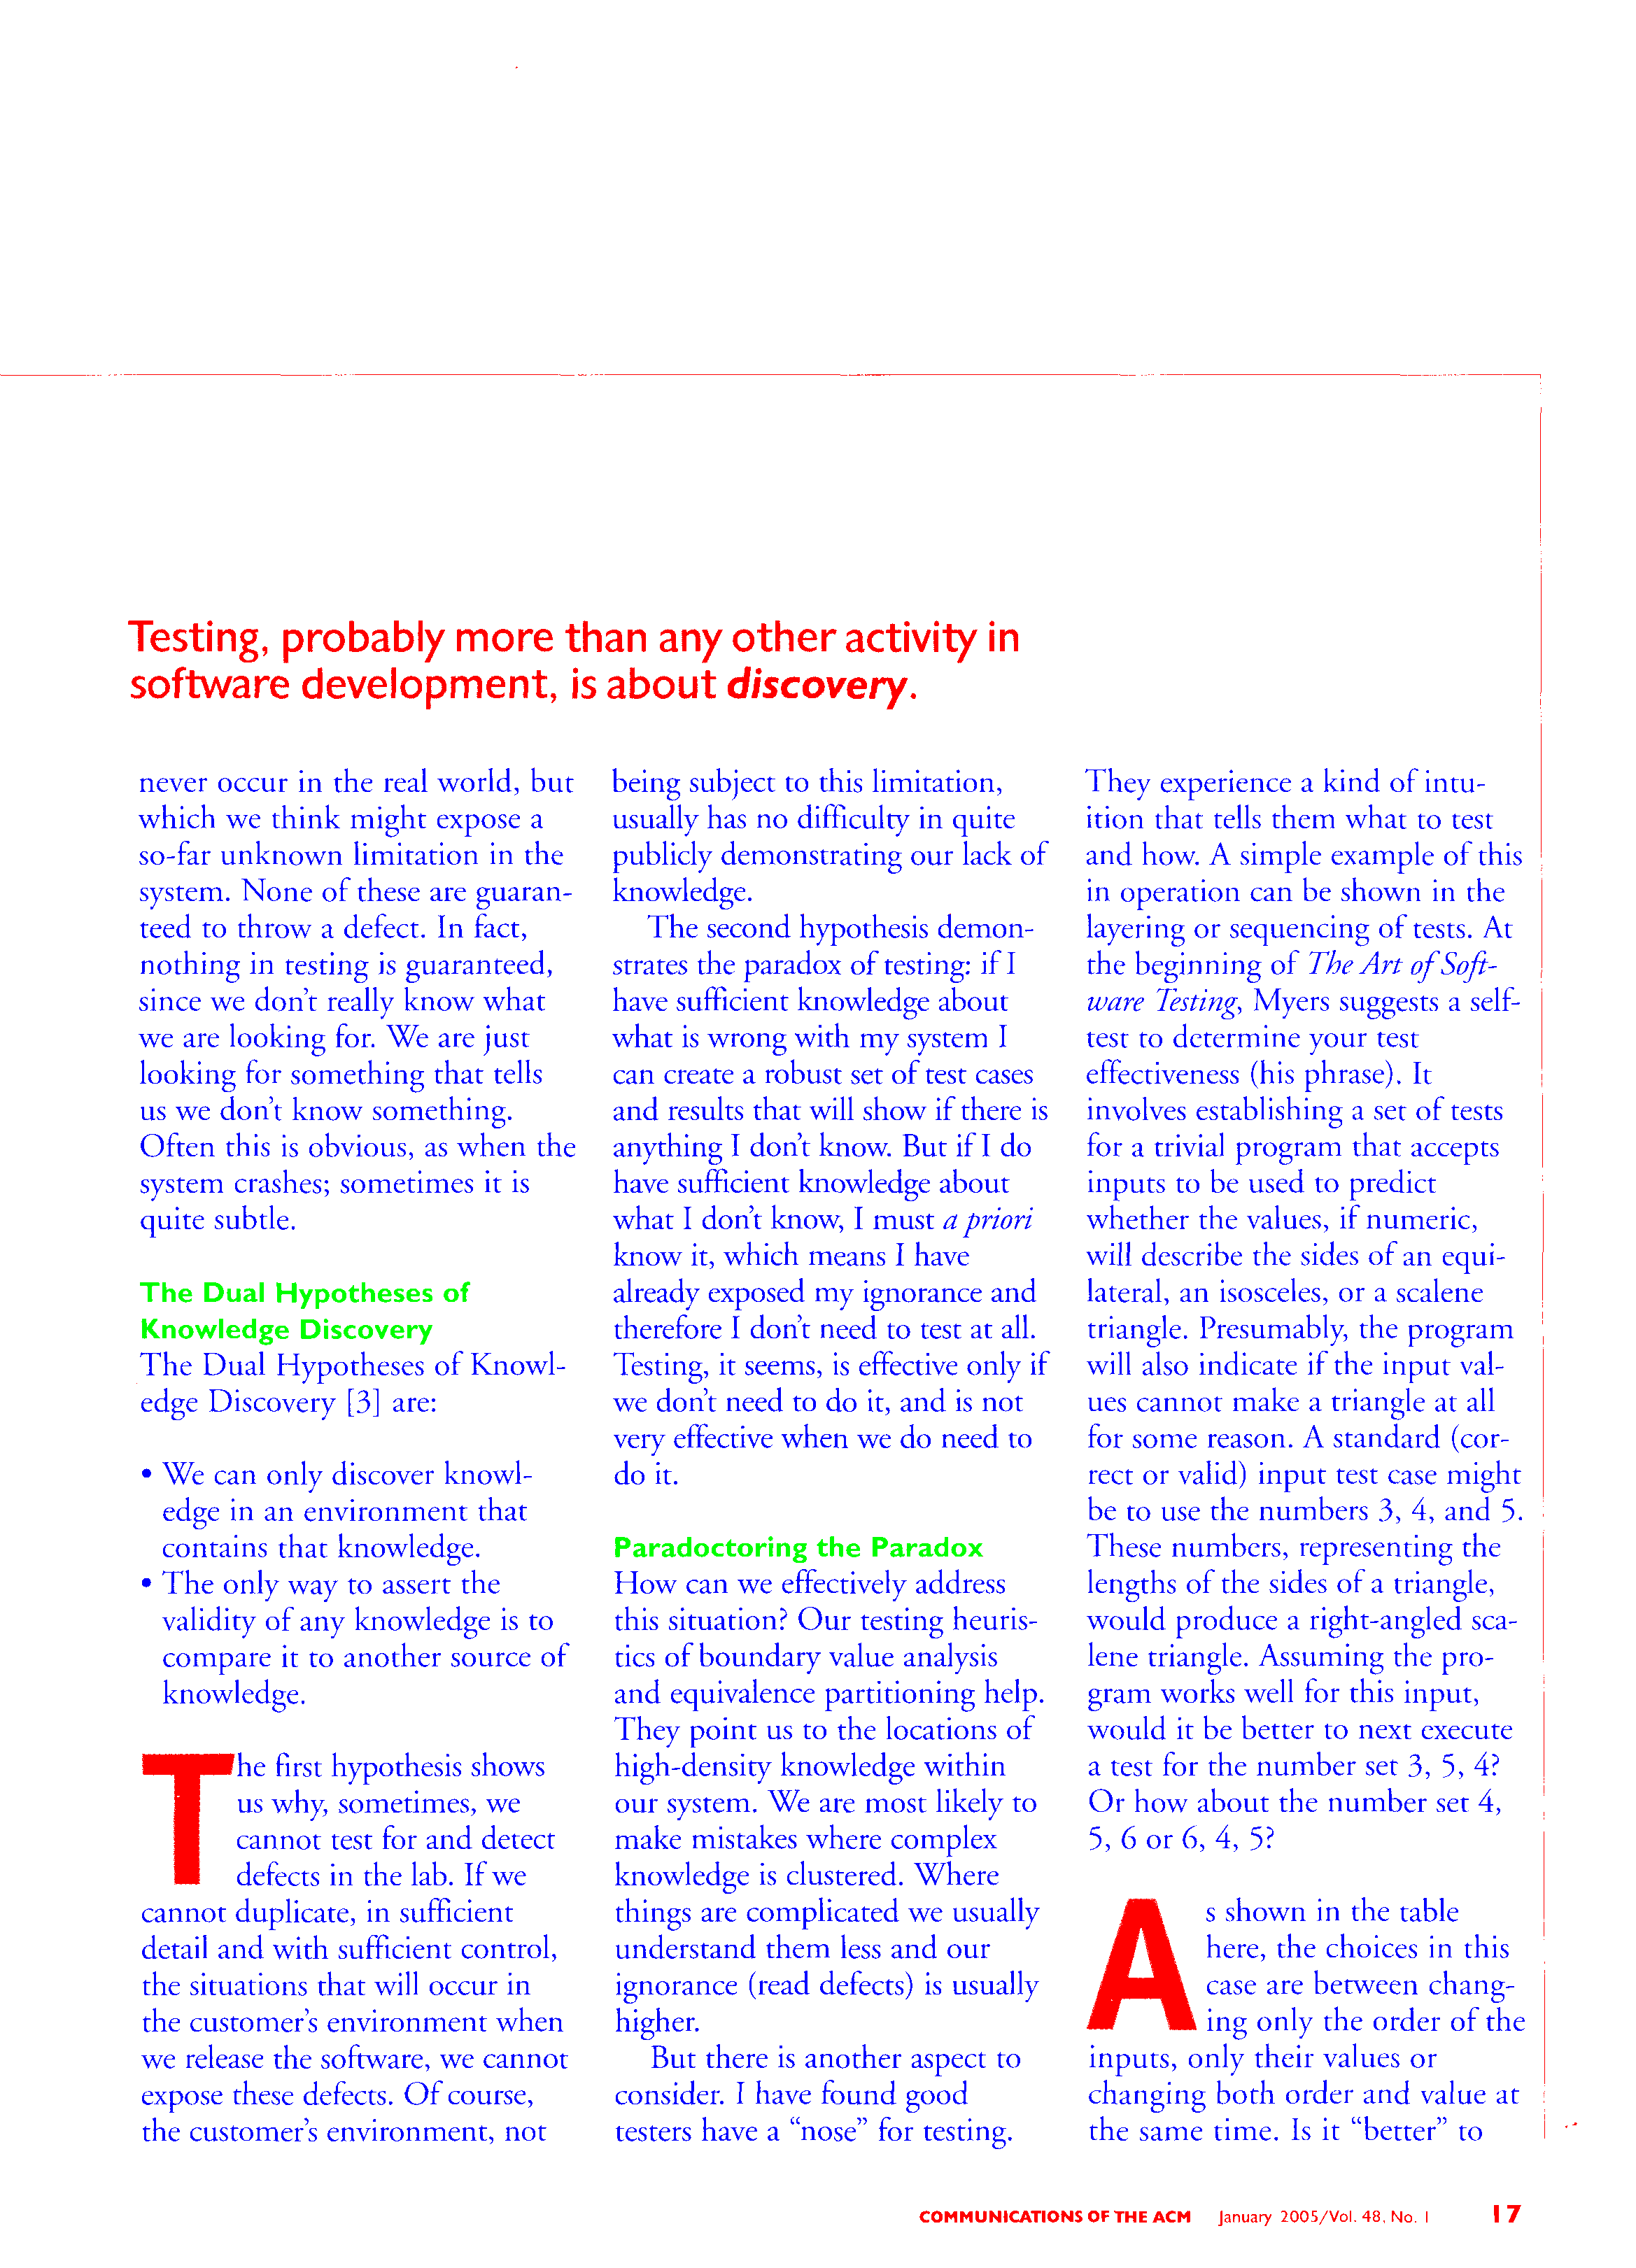
\includegraphics[width=0.4\textwidth]{assets/final_ideal/cacm_803_ideal.png}
        &
        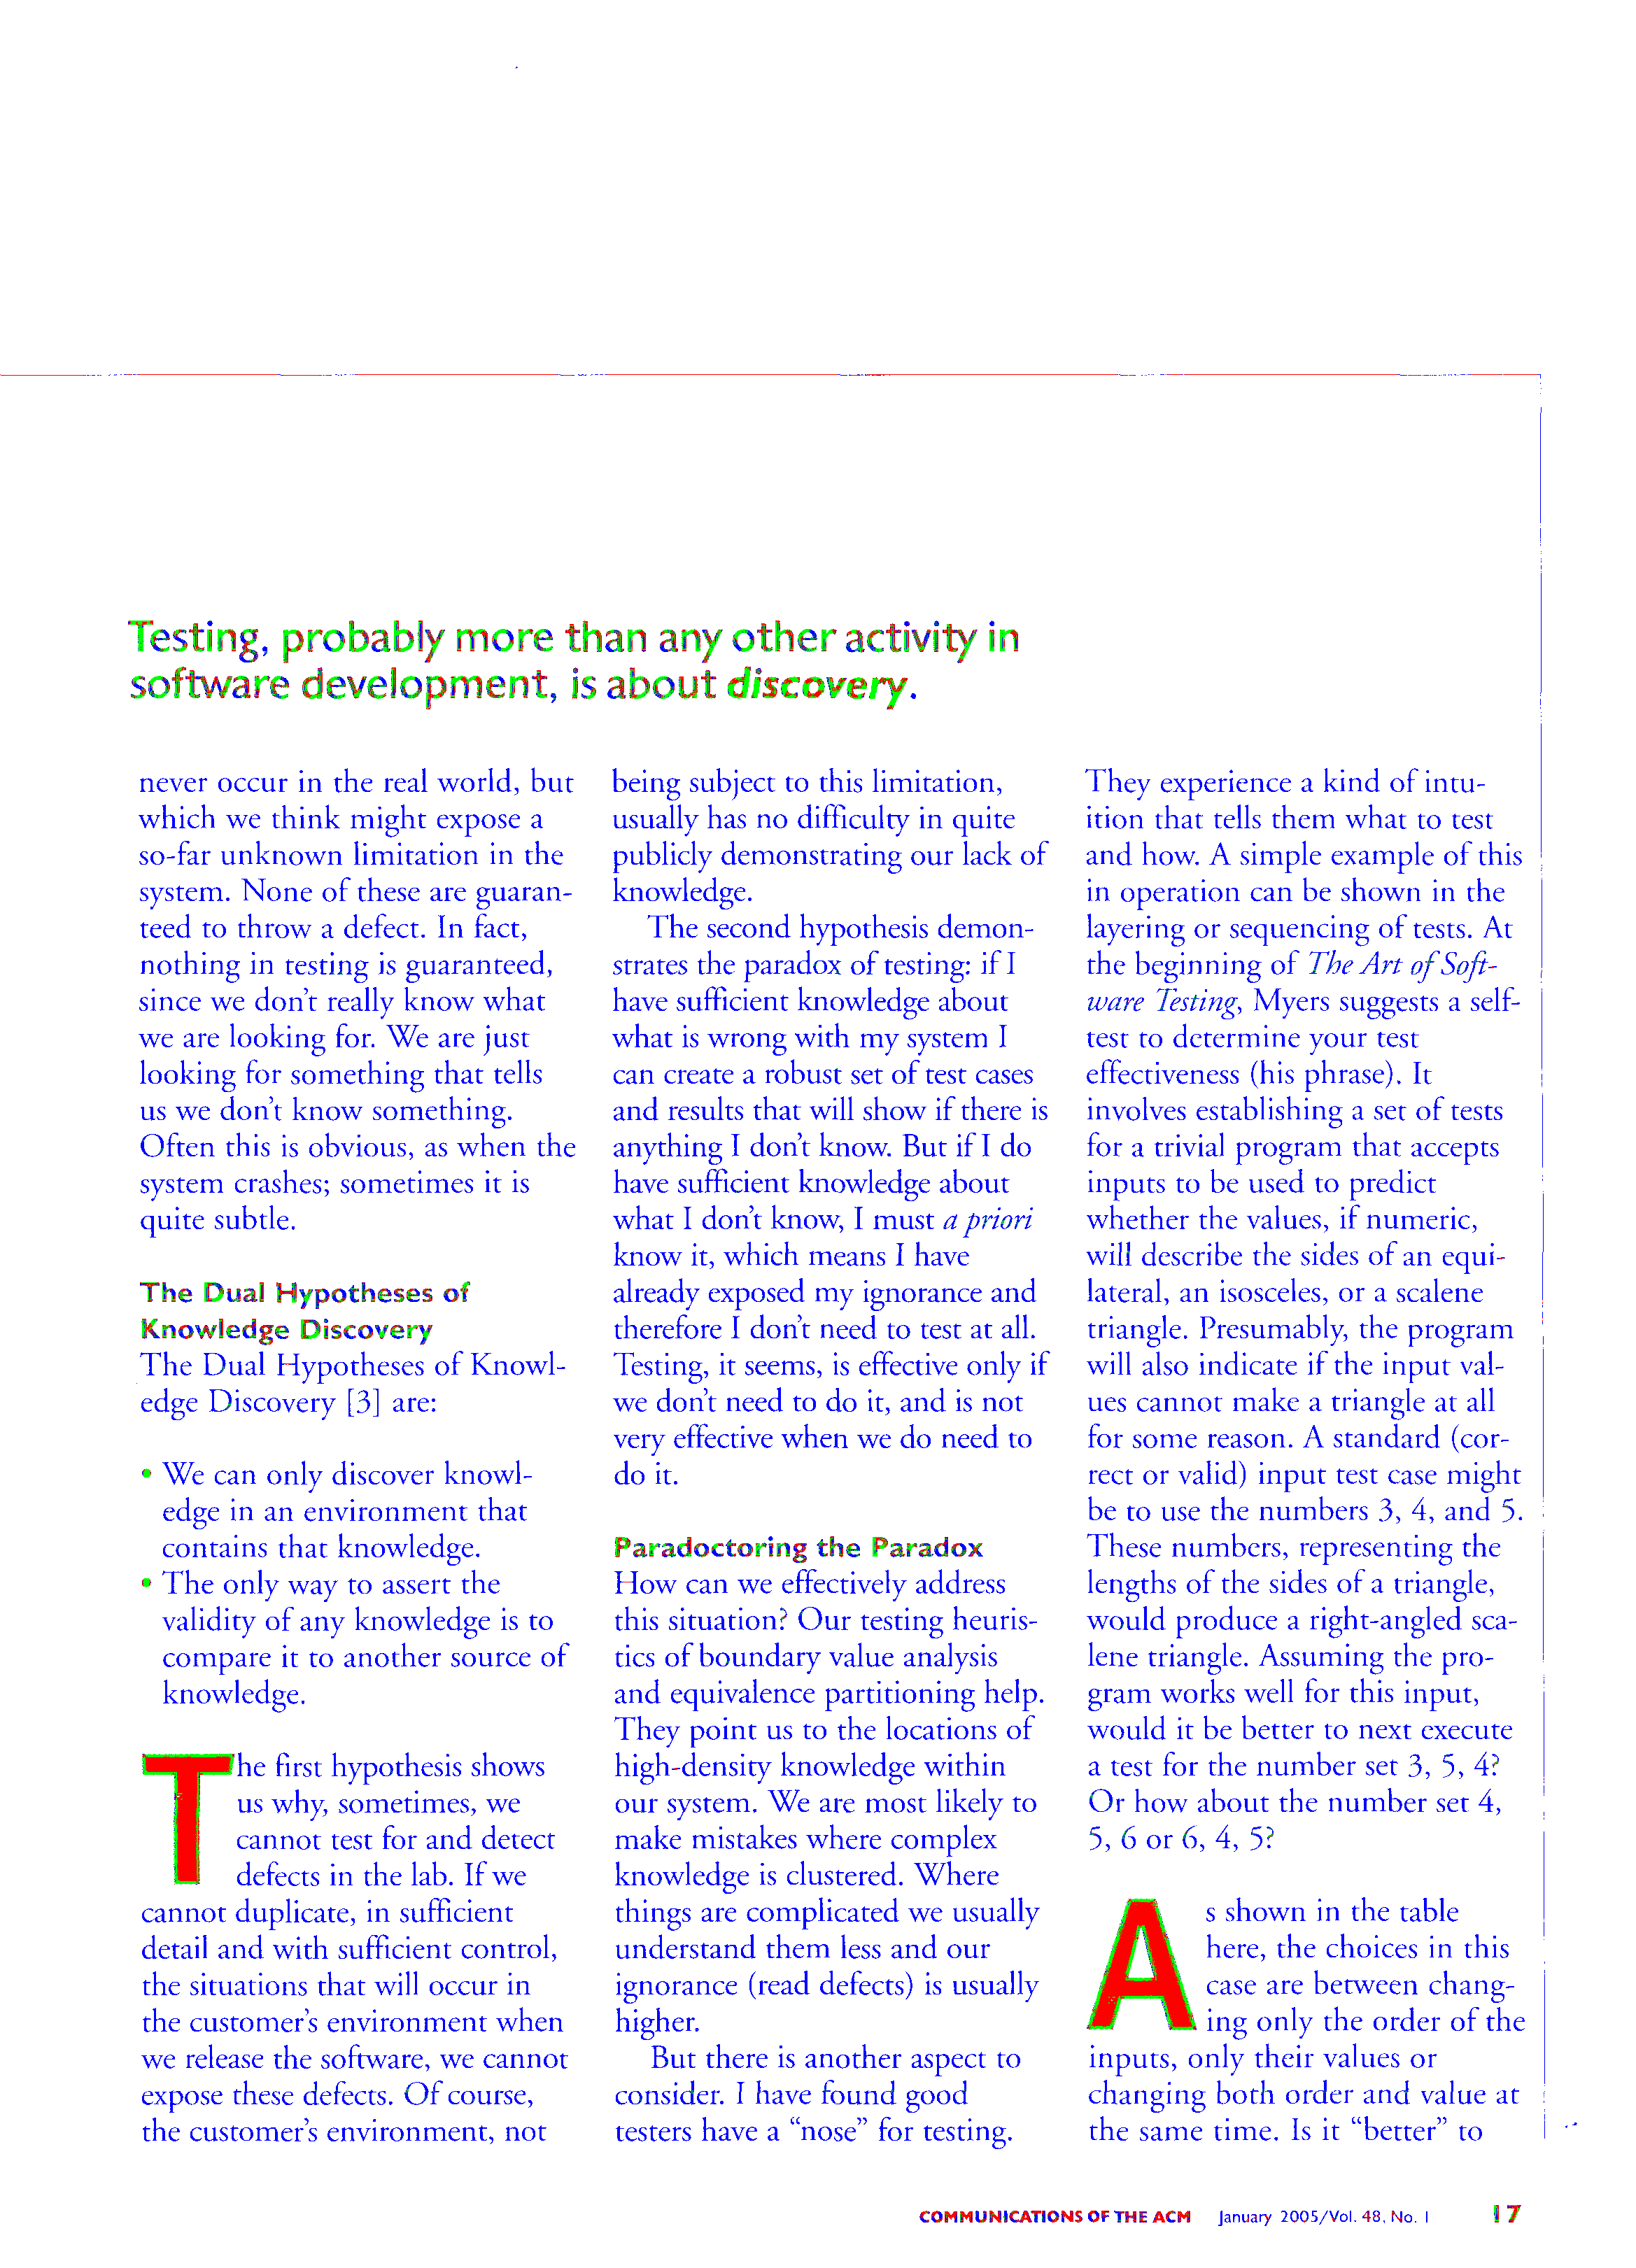
\includegraphics[width=0.4\textwidth]{assets/result_imagens/cacm_50_percent_sparse_9x9_803_final.png}
        \end{tabular}
      \end{center}
      \label{tab:segmentation_803}
    \end{table}

    % 
    % TIME
    % 

    \begin{table}[p]
      \caption{Segmentação da imagem 783}
      \begin{center}
        \begin{tabular}{ c c }
          Ideal & Segmentada \\
          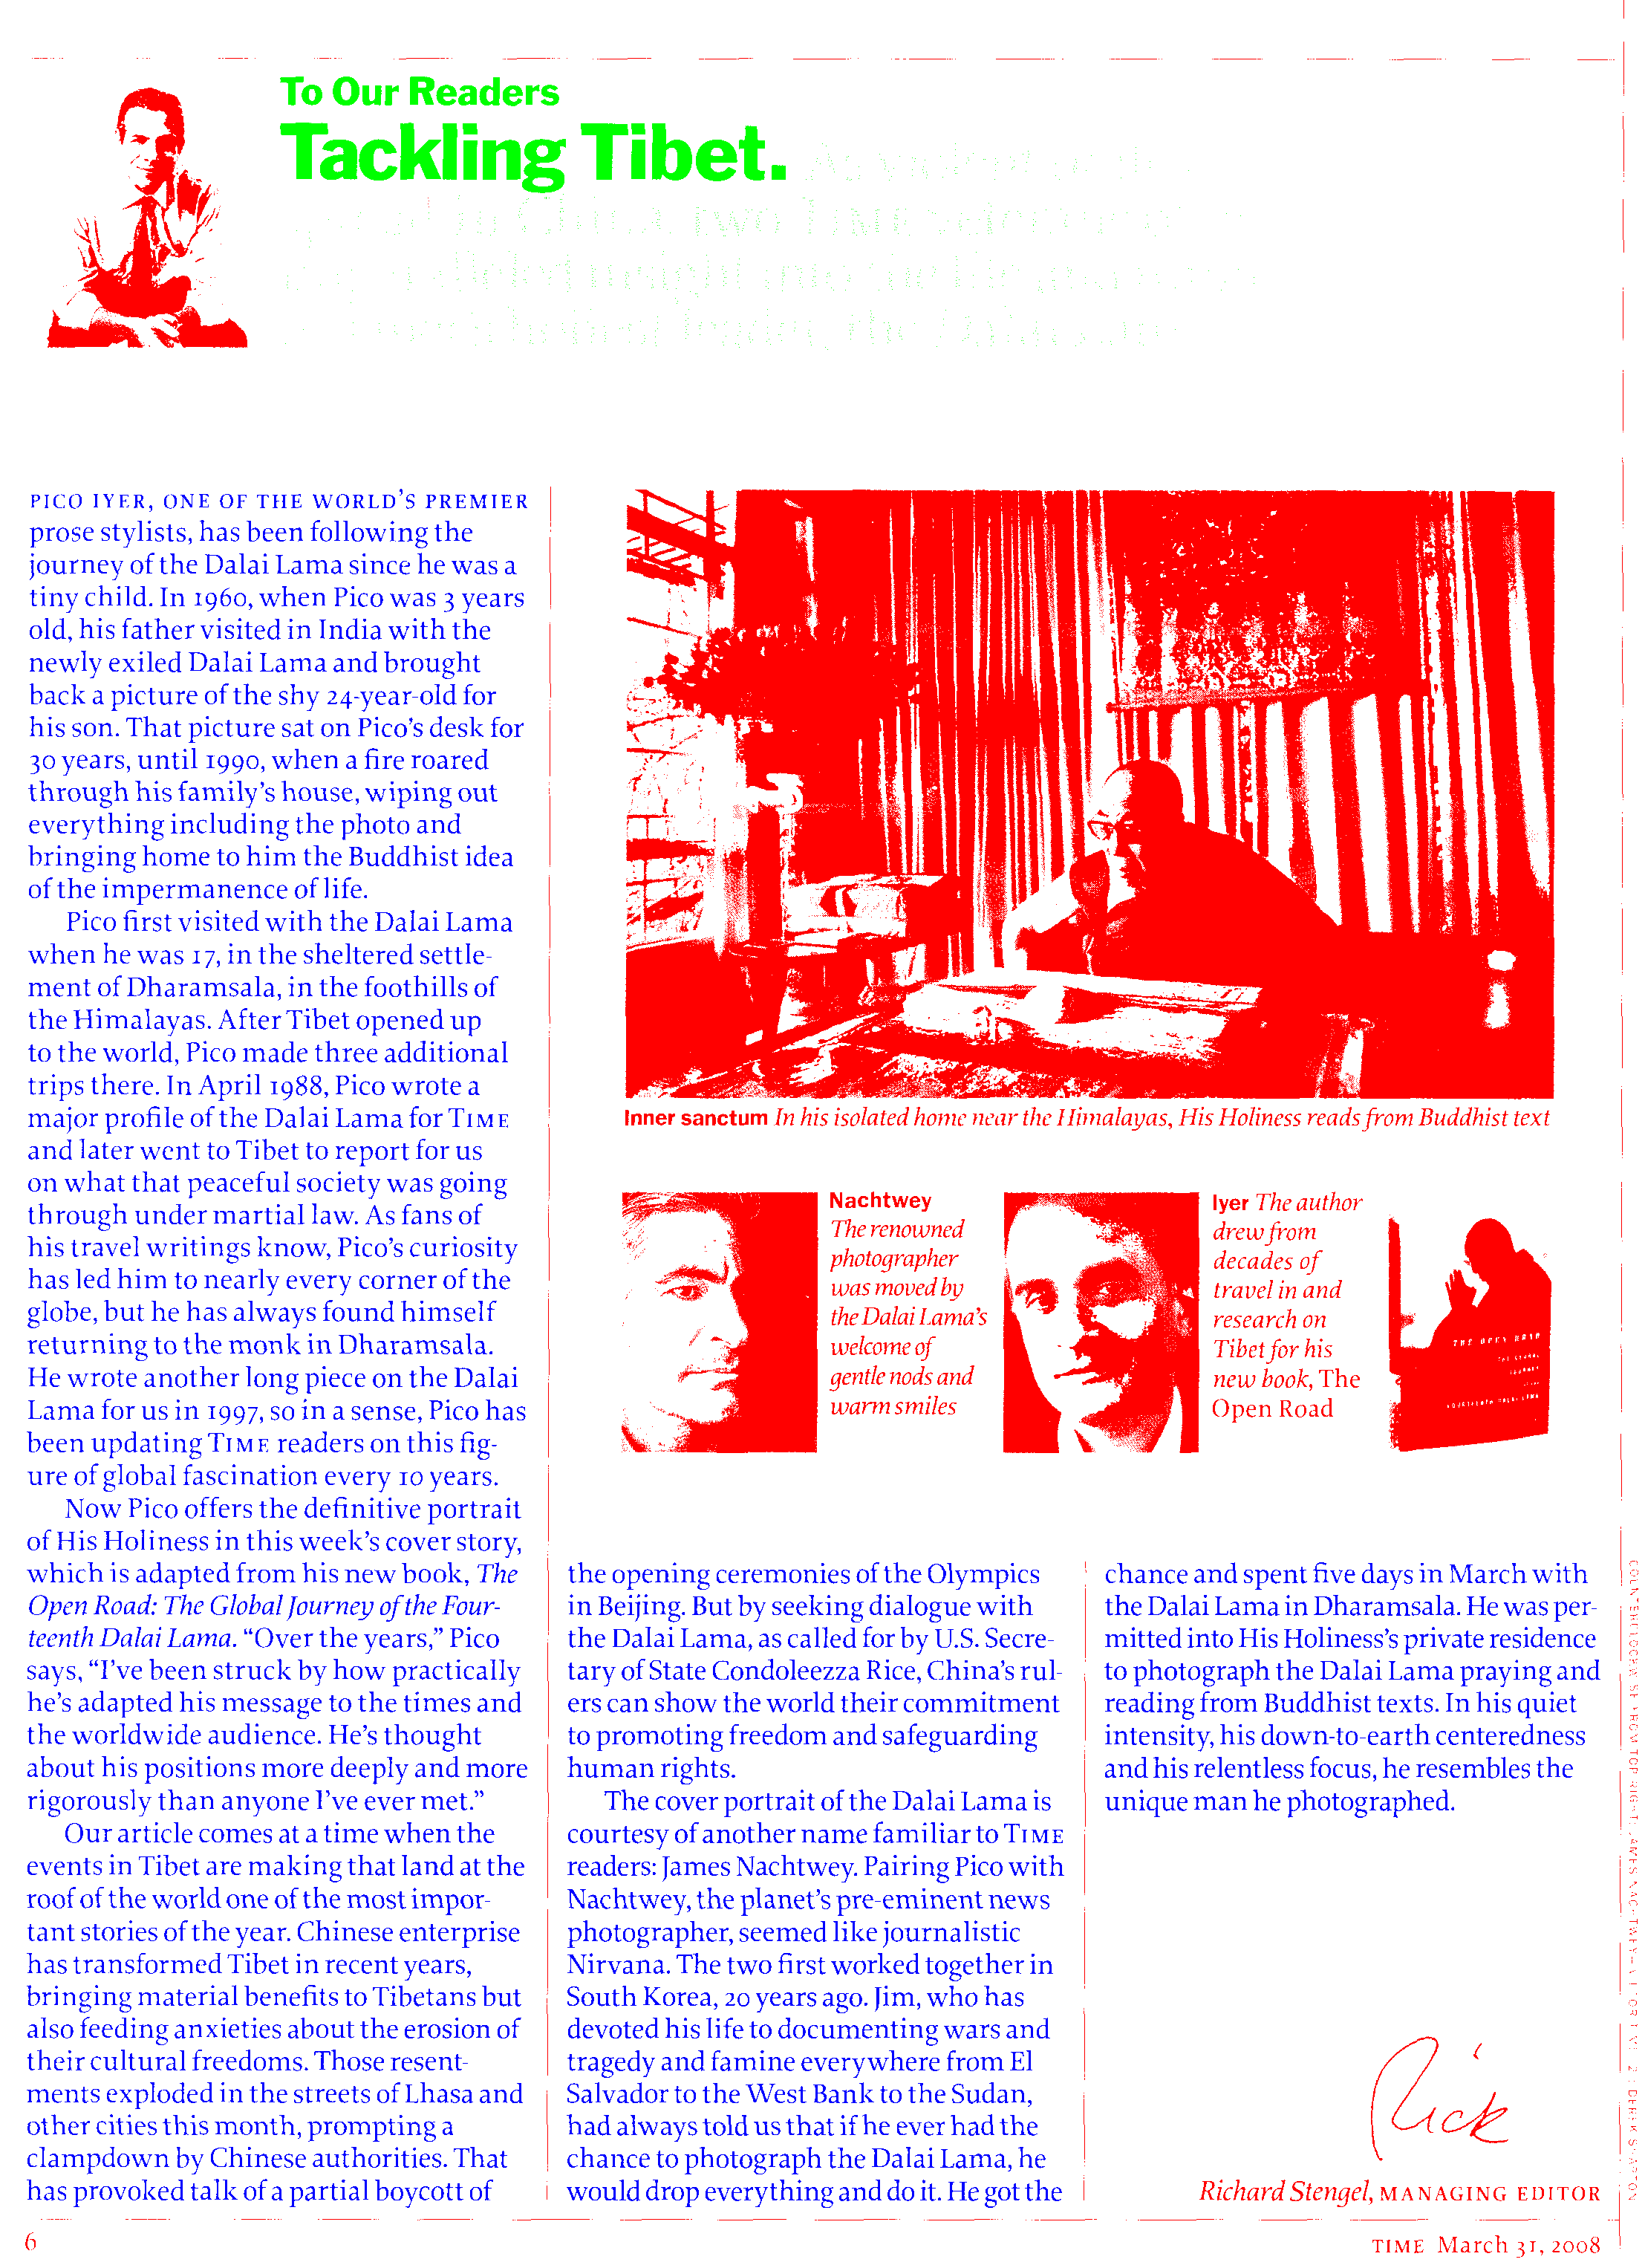
\includegraphics[width=0.4\textwidth]{assets/final_ideal/time_783_ideal.png}
          &
          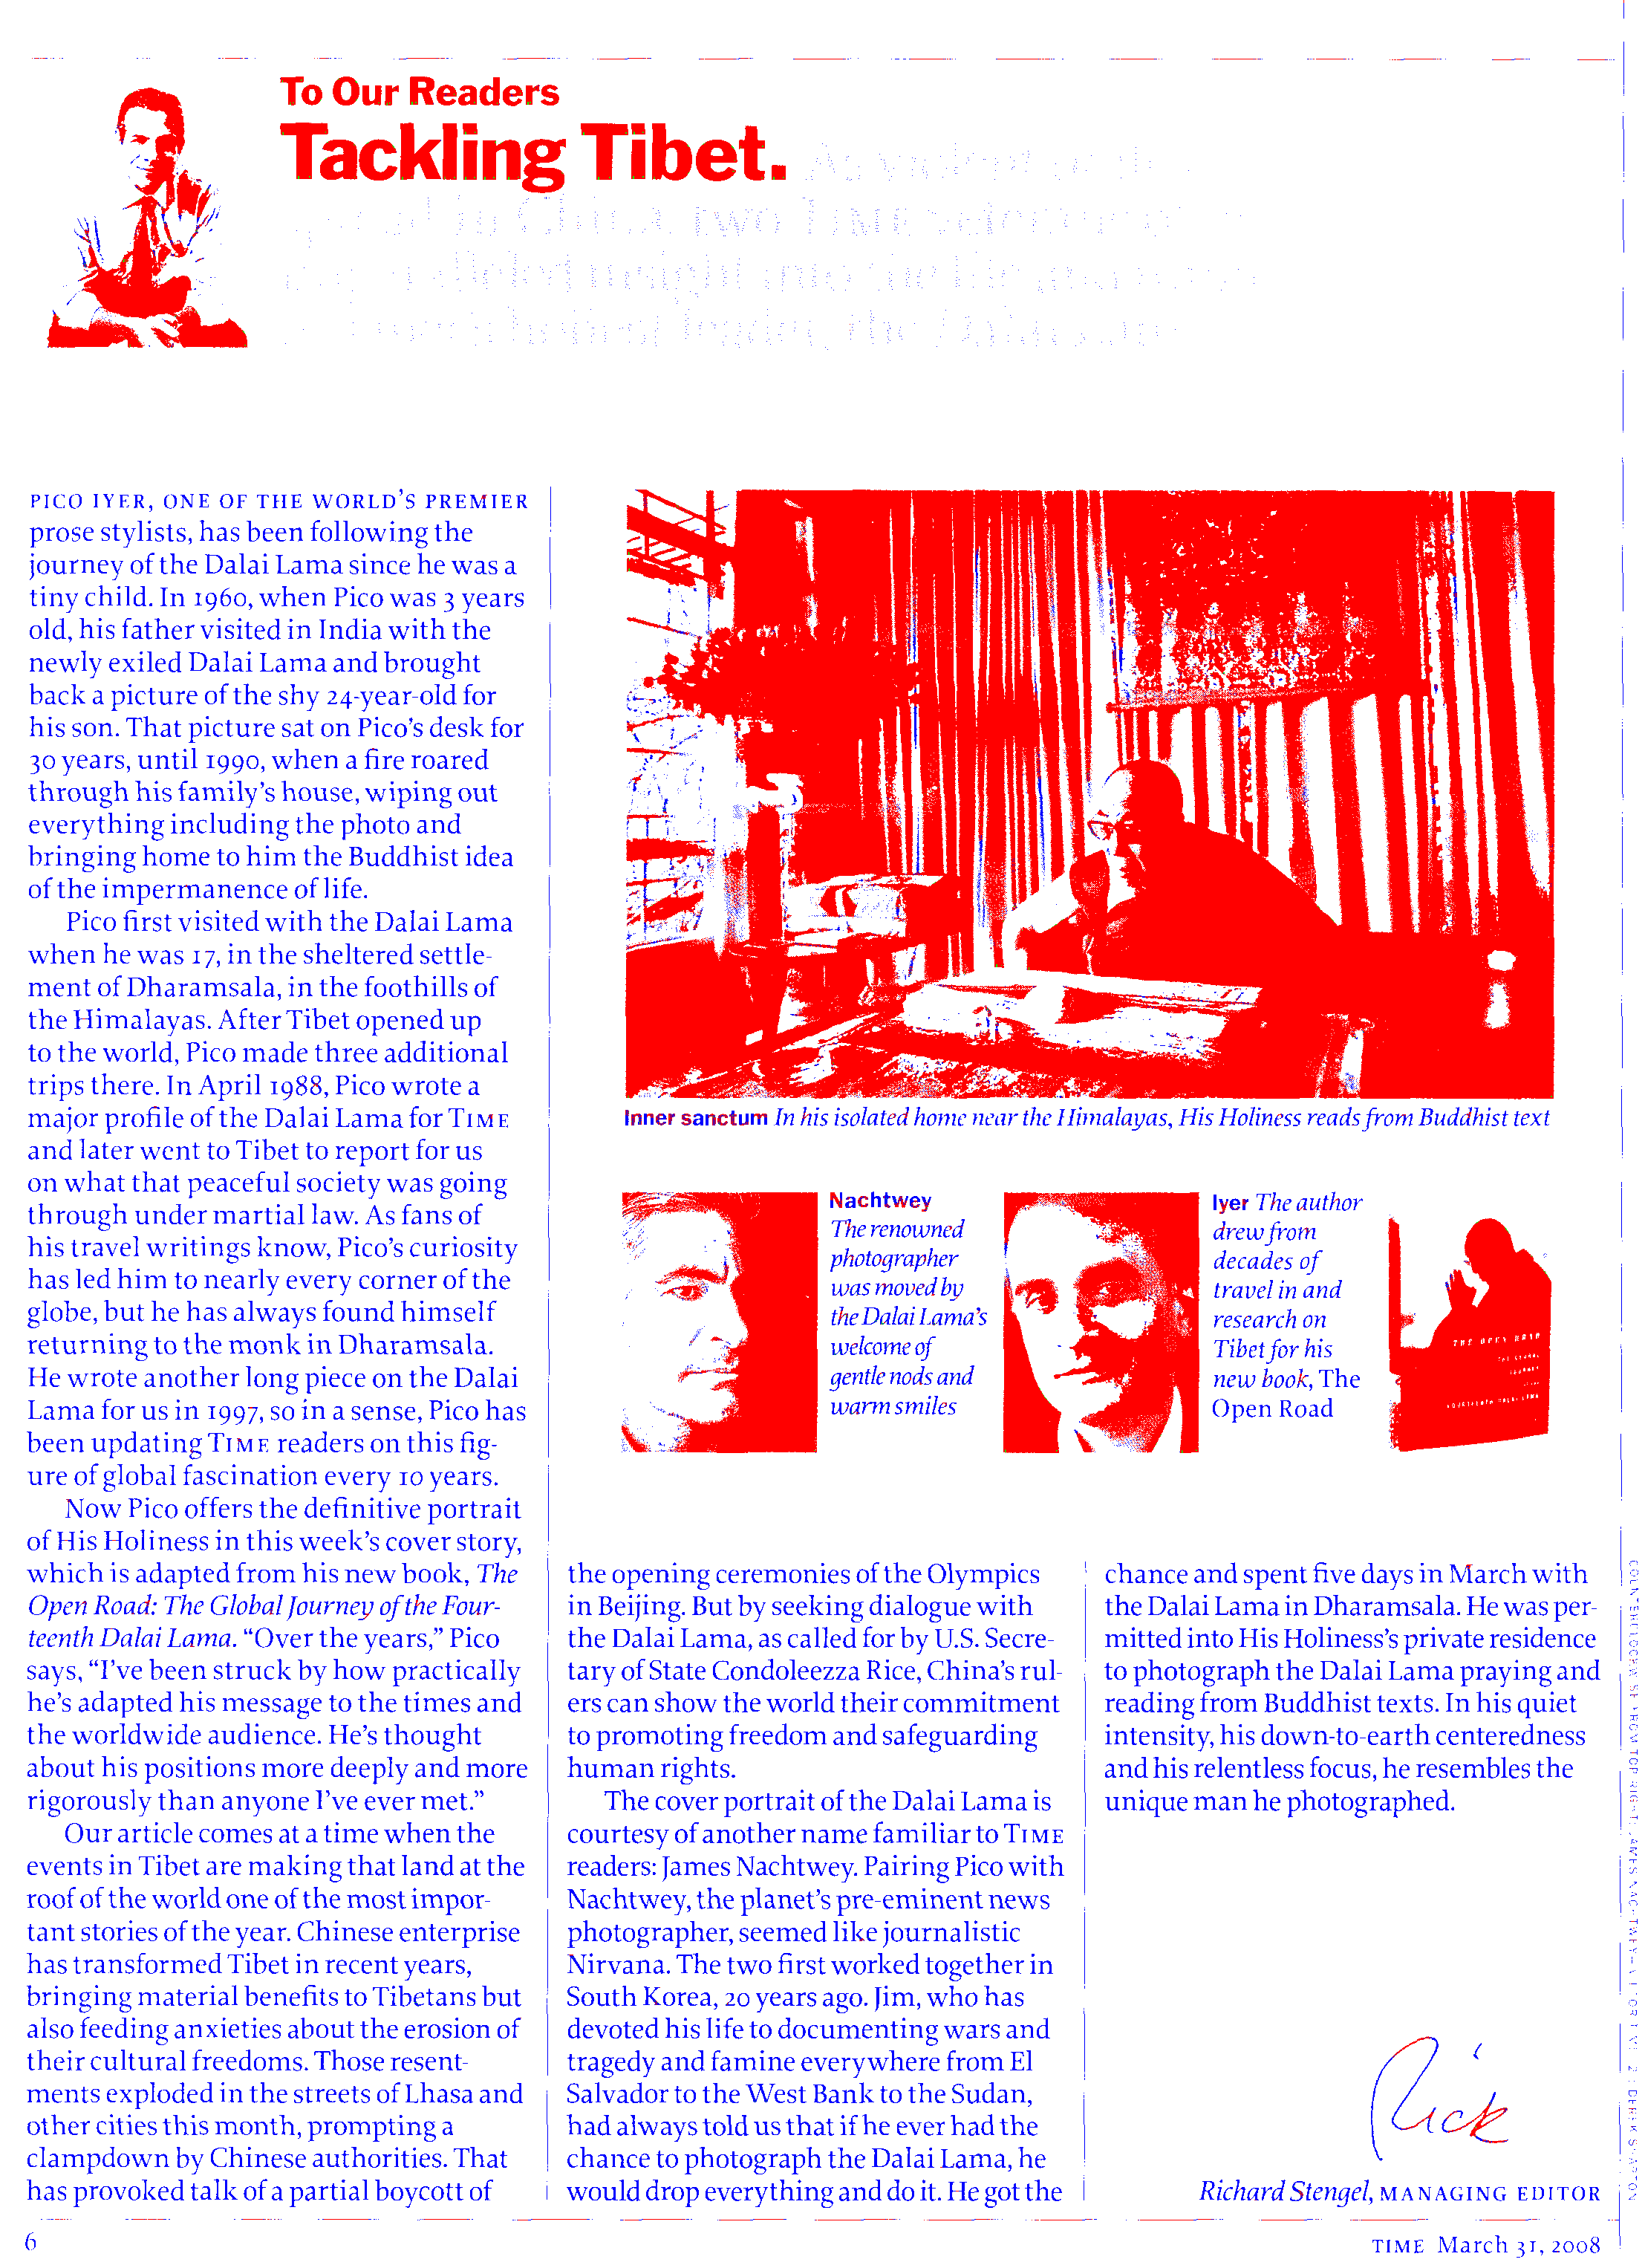
\includegraphics[width=0.4\textwidth]{assets/result_imagens/time_50_percent_sparse_9x9_783_final.png}
        \end{tabular}
      \end{center}
      \label{tab:segmentation_783}
    \end{table}
    \begin{table}[p]
      \caption{Segmentação da imagem 784}
      \begin{center}
        \begin{tabular}{ c c }
          Ideal & Segmentada \\
          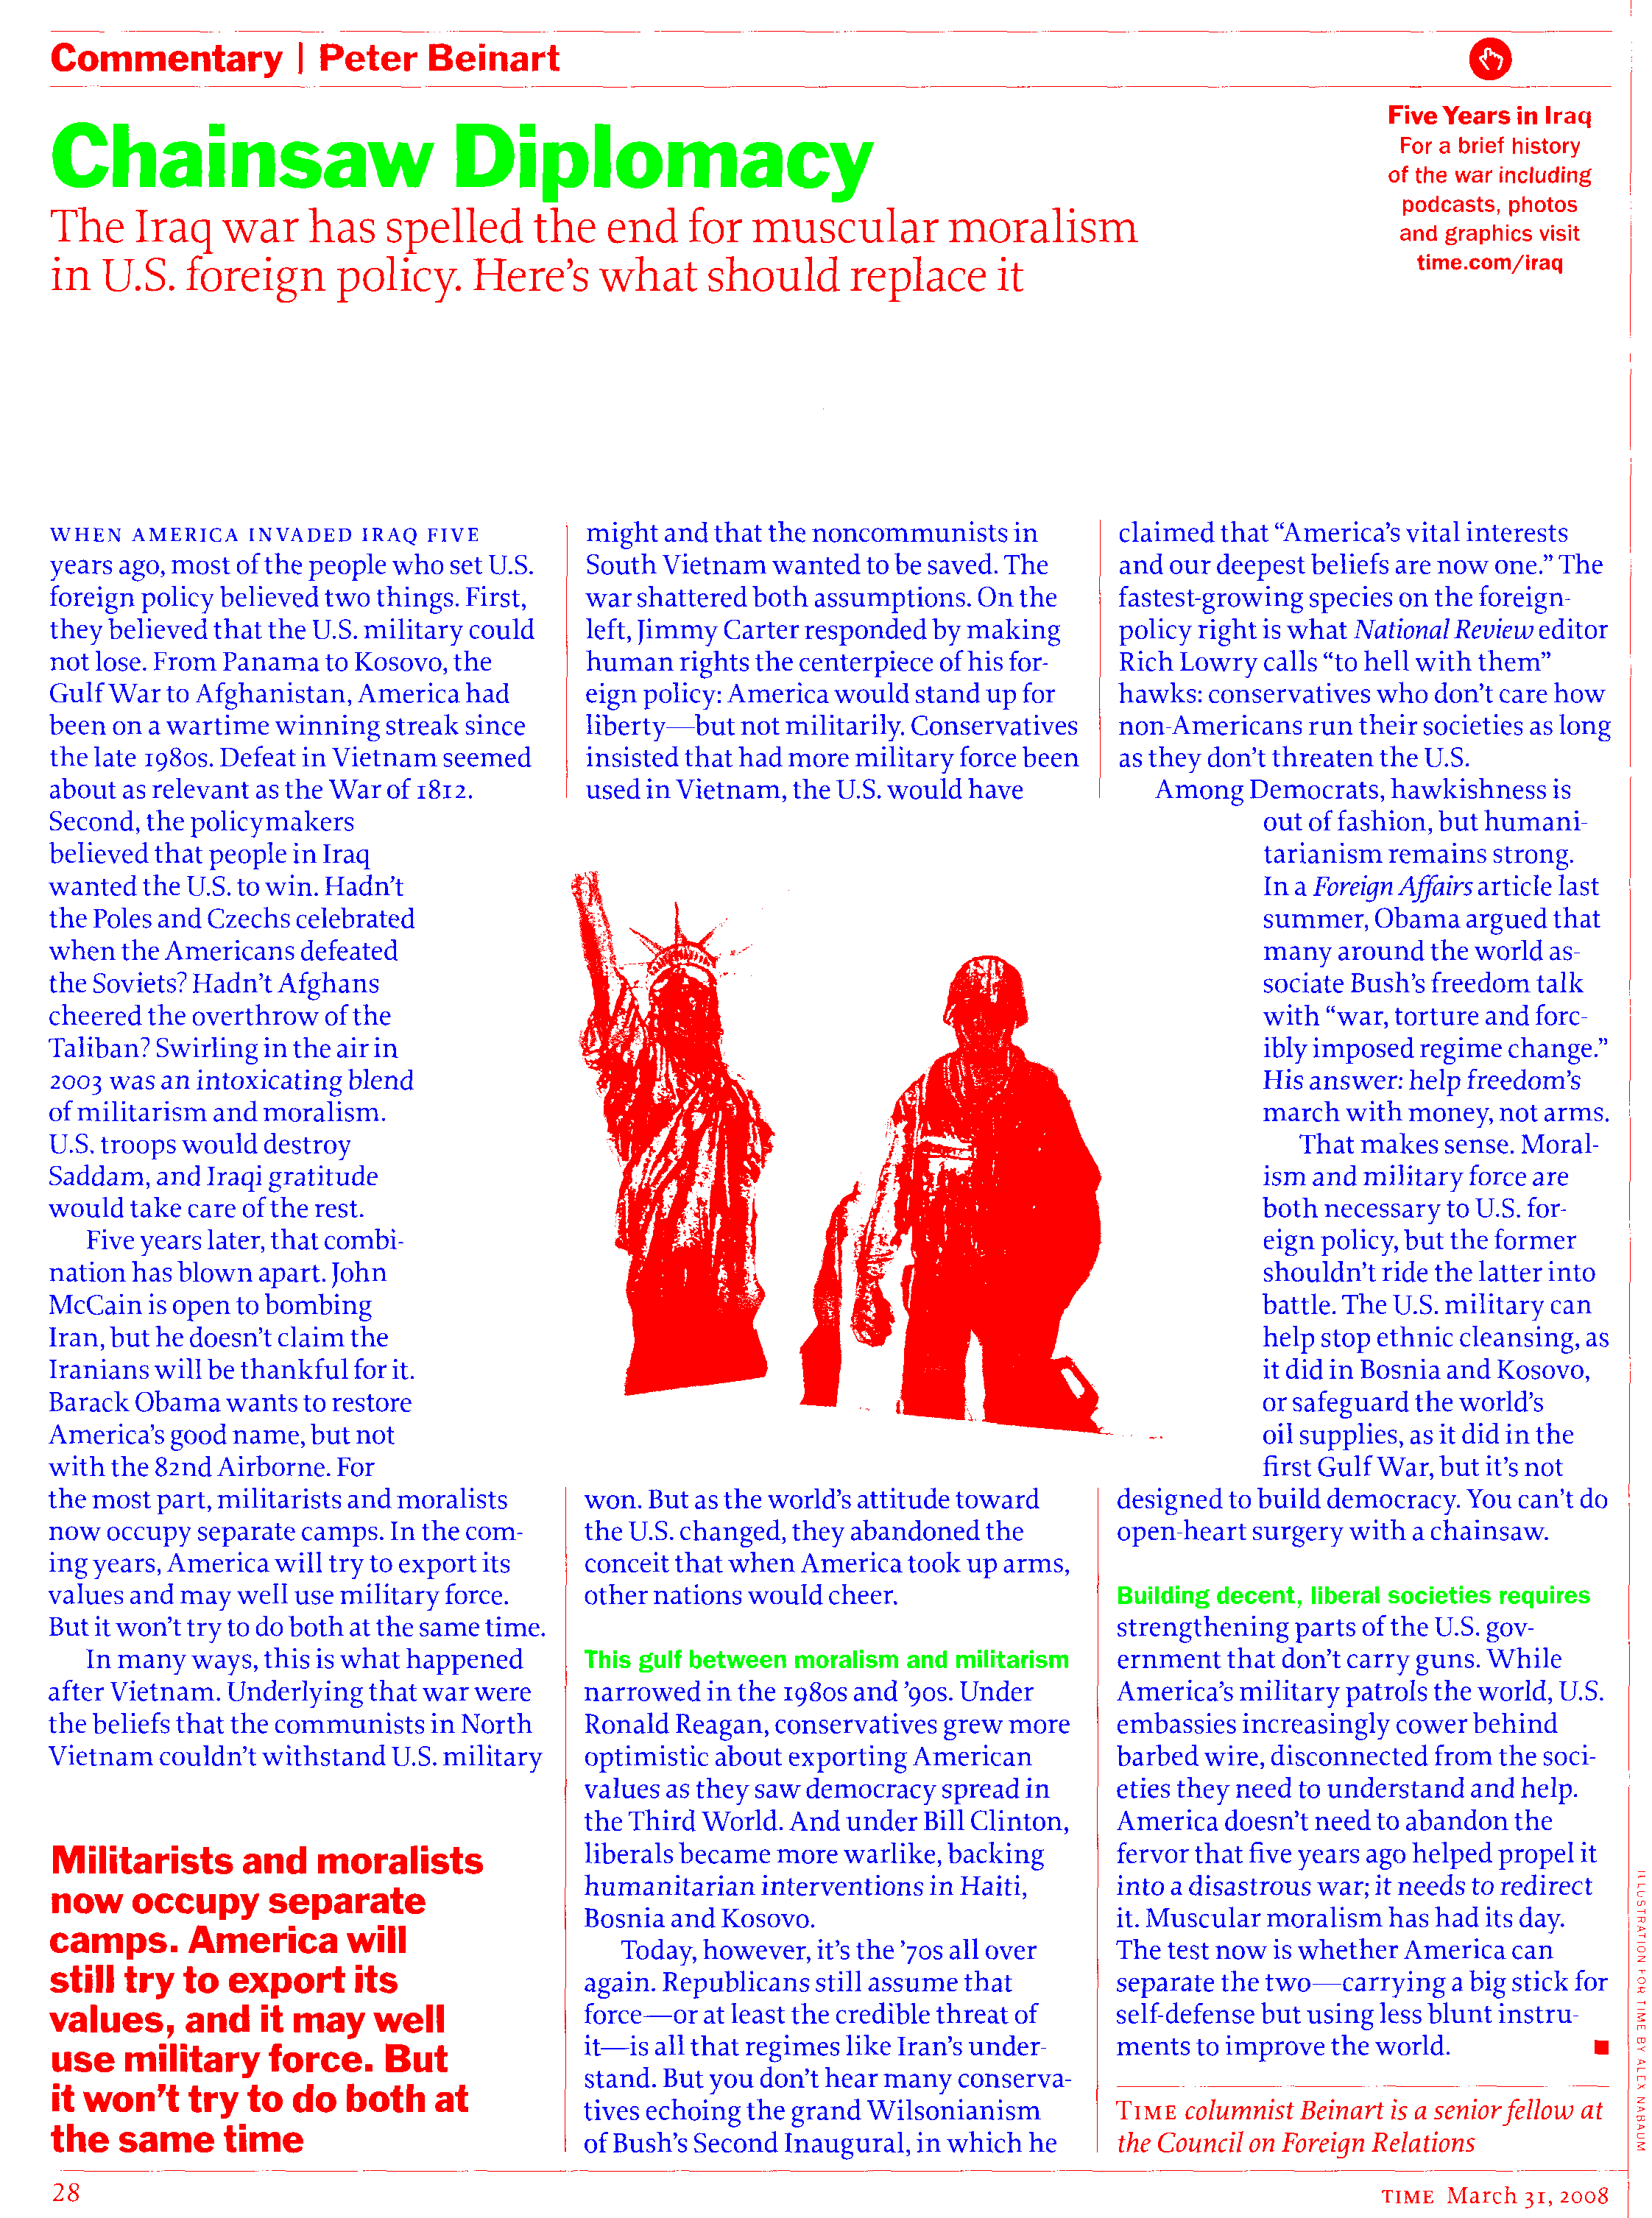
\includegraphics[width=0.4\textwidth]{assets/final_ideal/time_784_ideal.png}
          &
          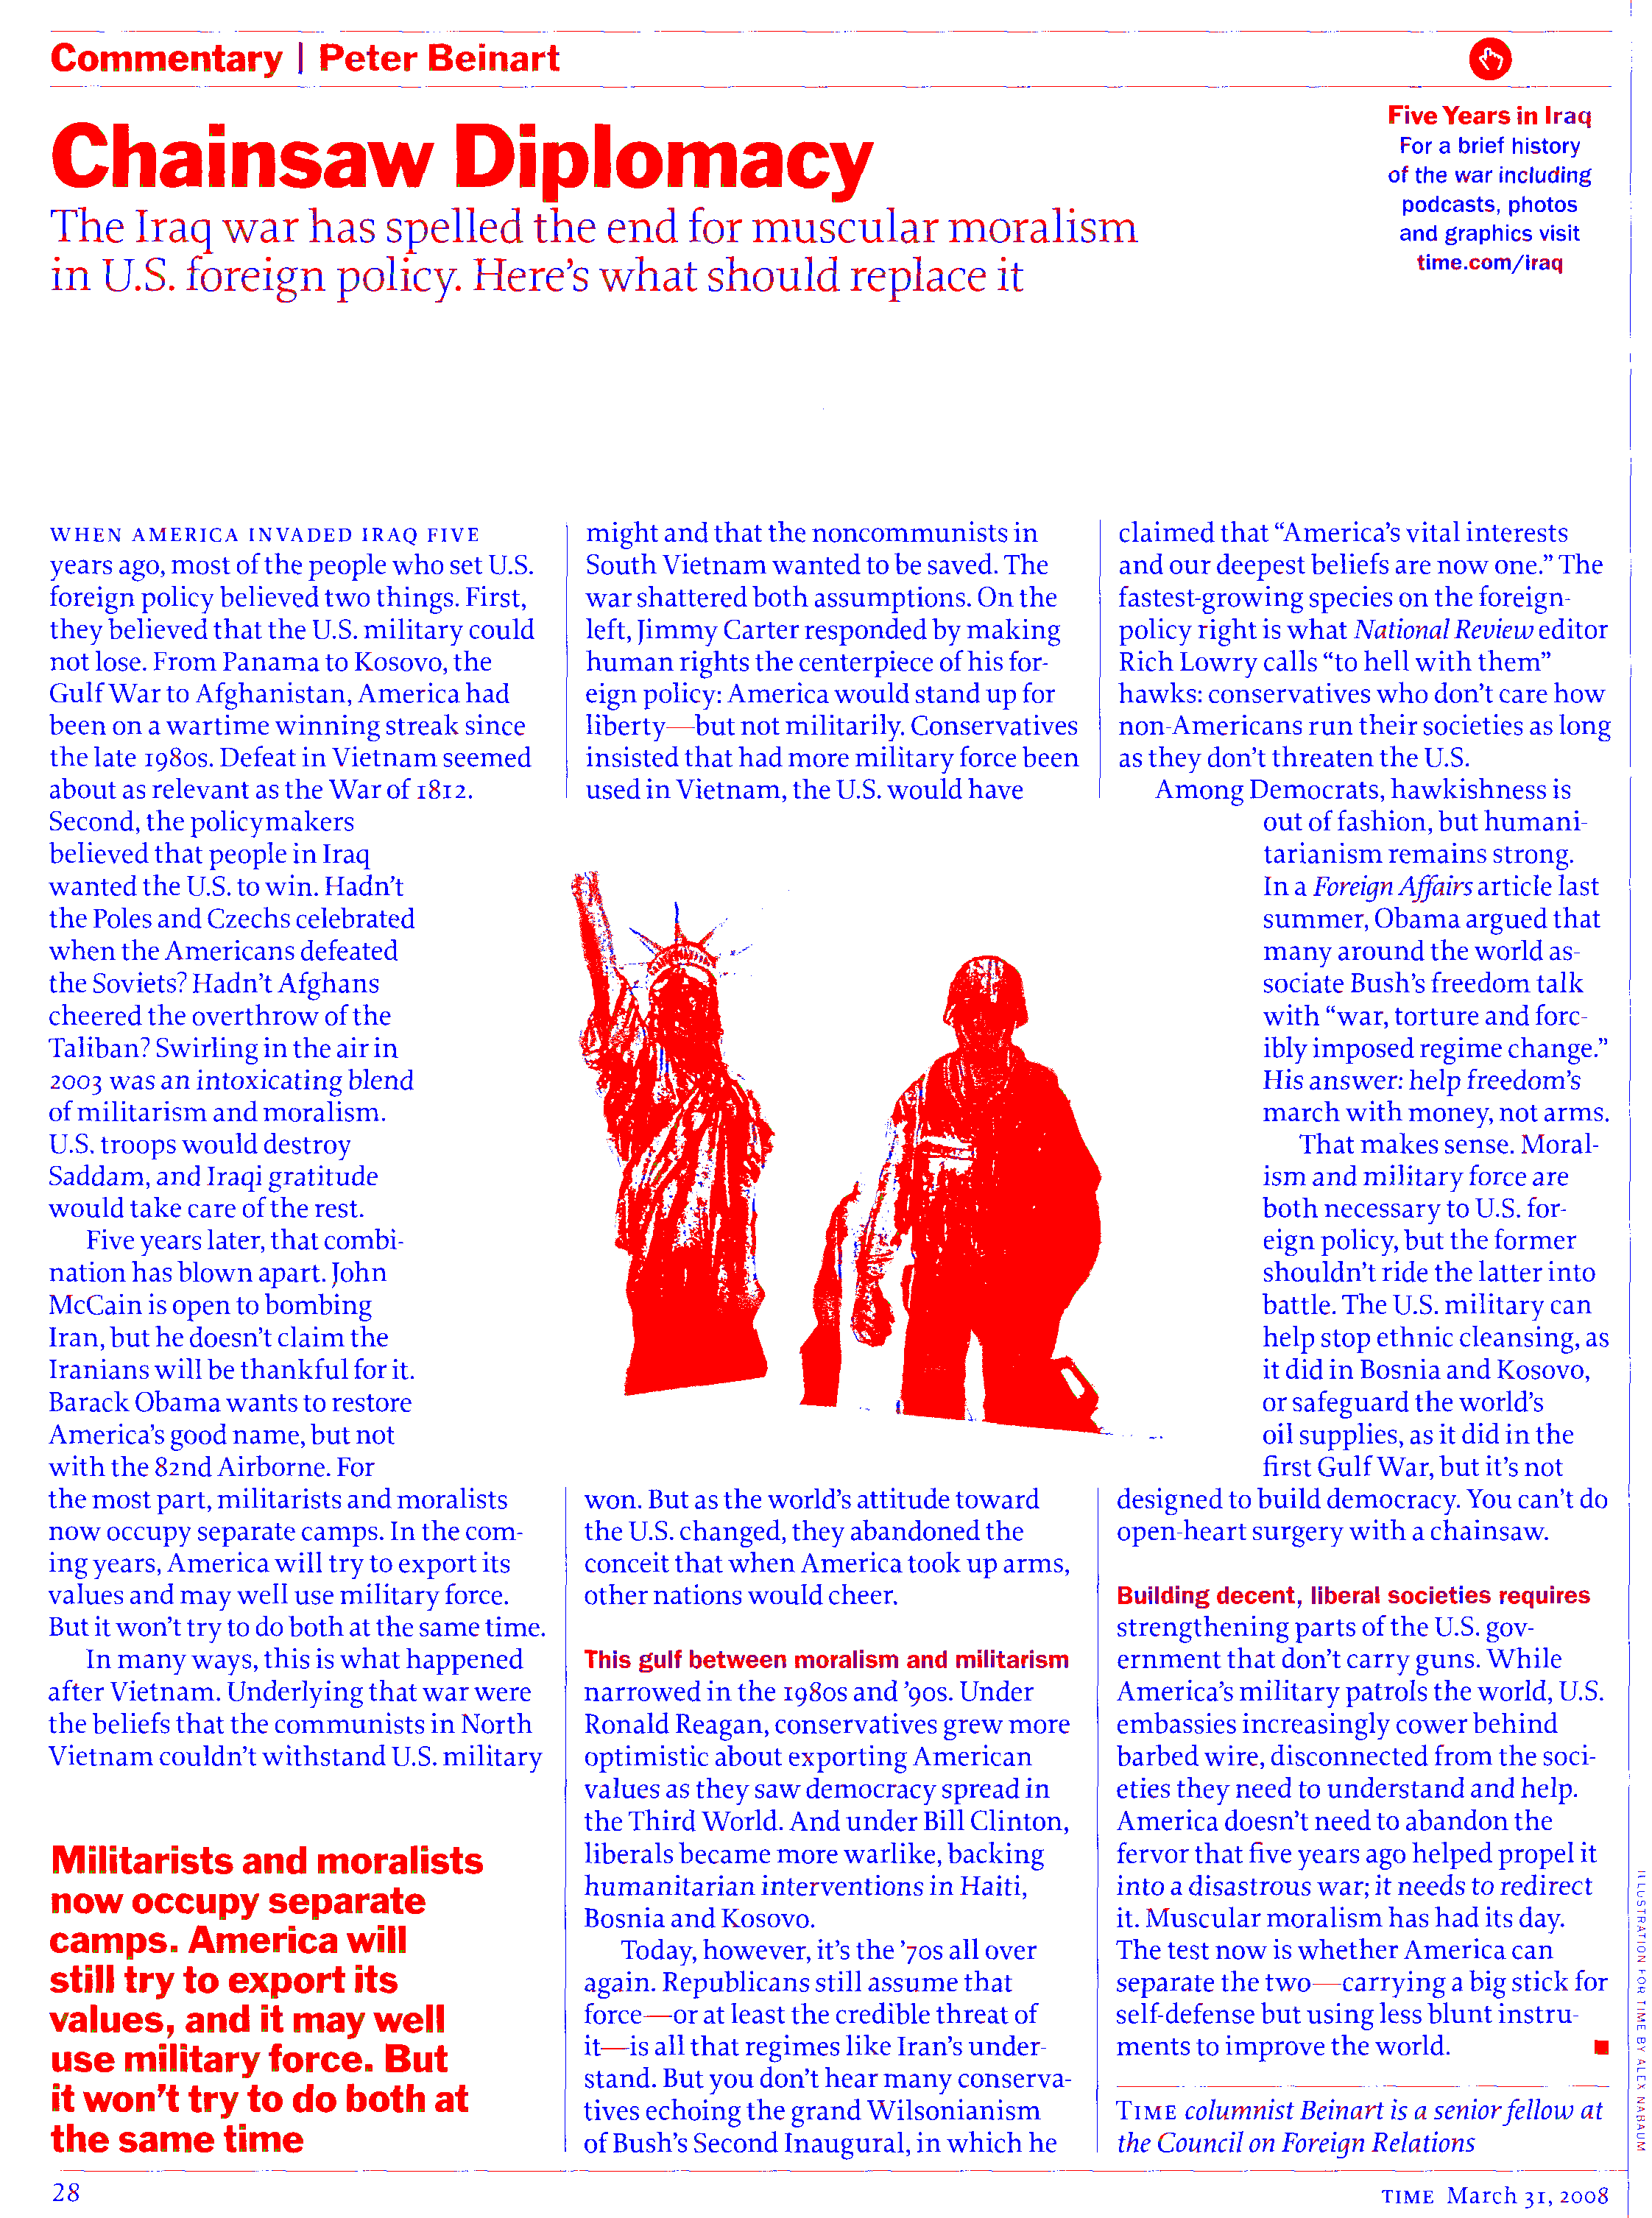
\includegraphics[width=0.4\textwidth]{assets/result_imagens/time_50_percent_sparse_9x9_784_final.png}
        \end{tabular}
      \end{center}
      \label{tab:segmentation_784}
    \end{table}
    \begin{table}[p]
      \caption{Segmentação da imagem 785}
      \begin{center}
        \begin{tabular}{ c c }
          Ideal & Segmentada \\
          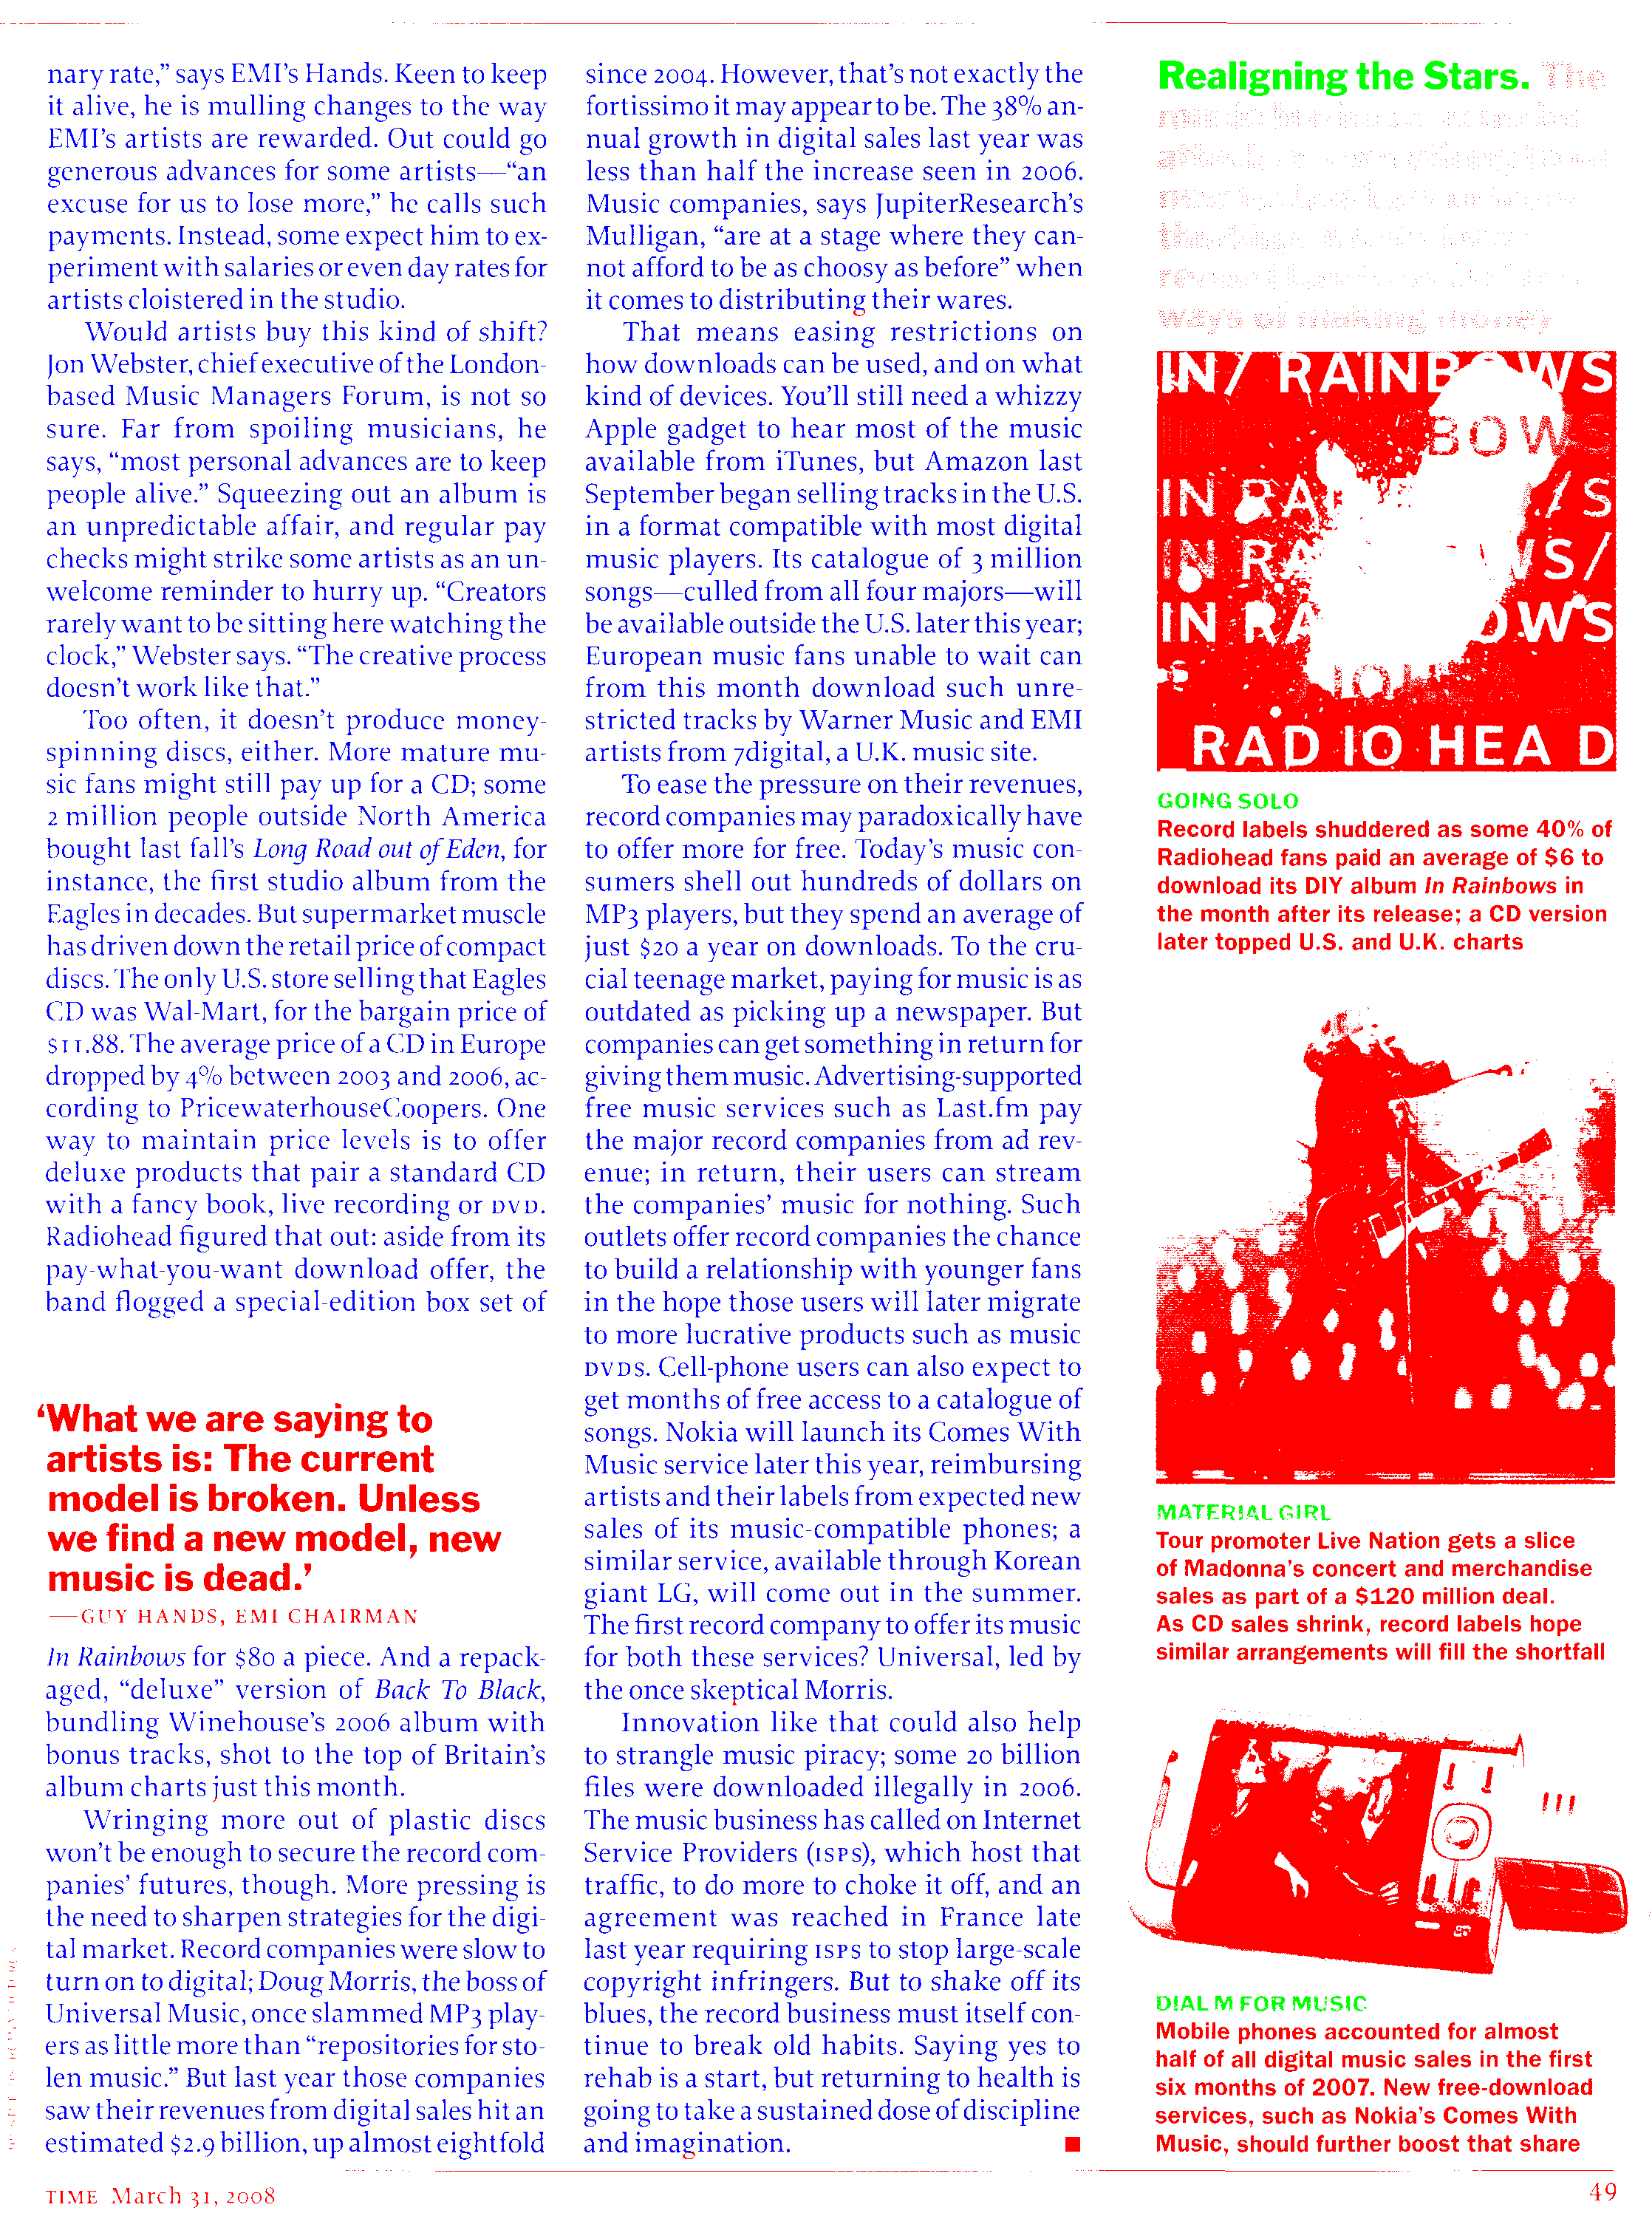
\includegraphics[width=0.4\textwidth]{assets/final_ideal/time_785_ideal.png}
          &
          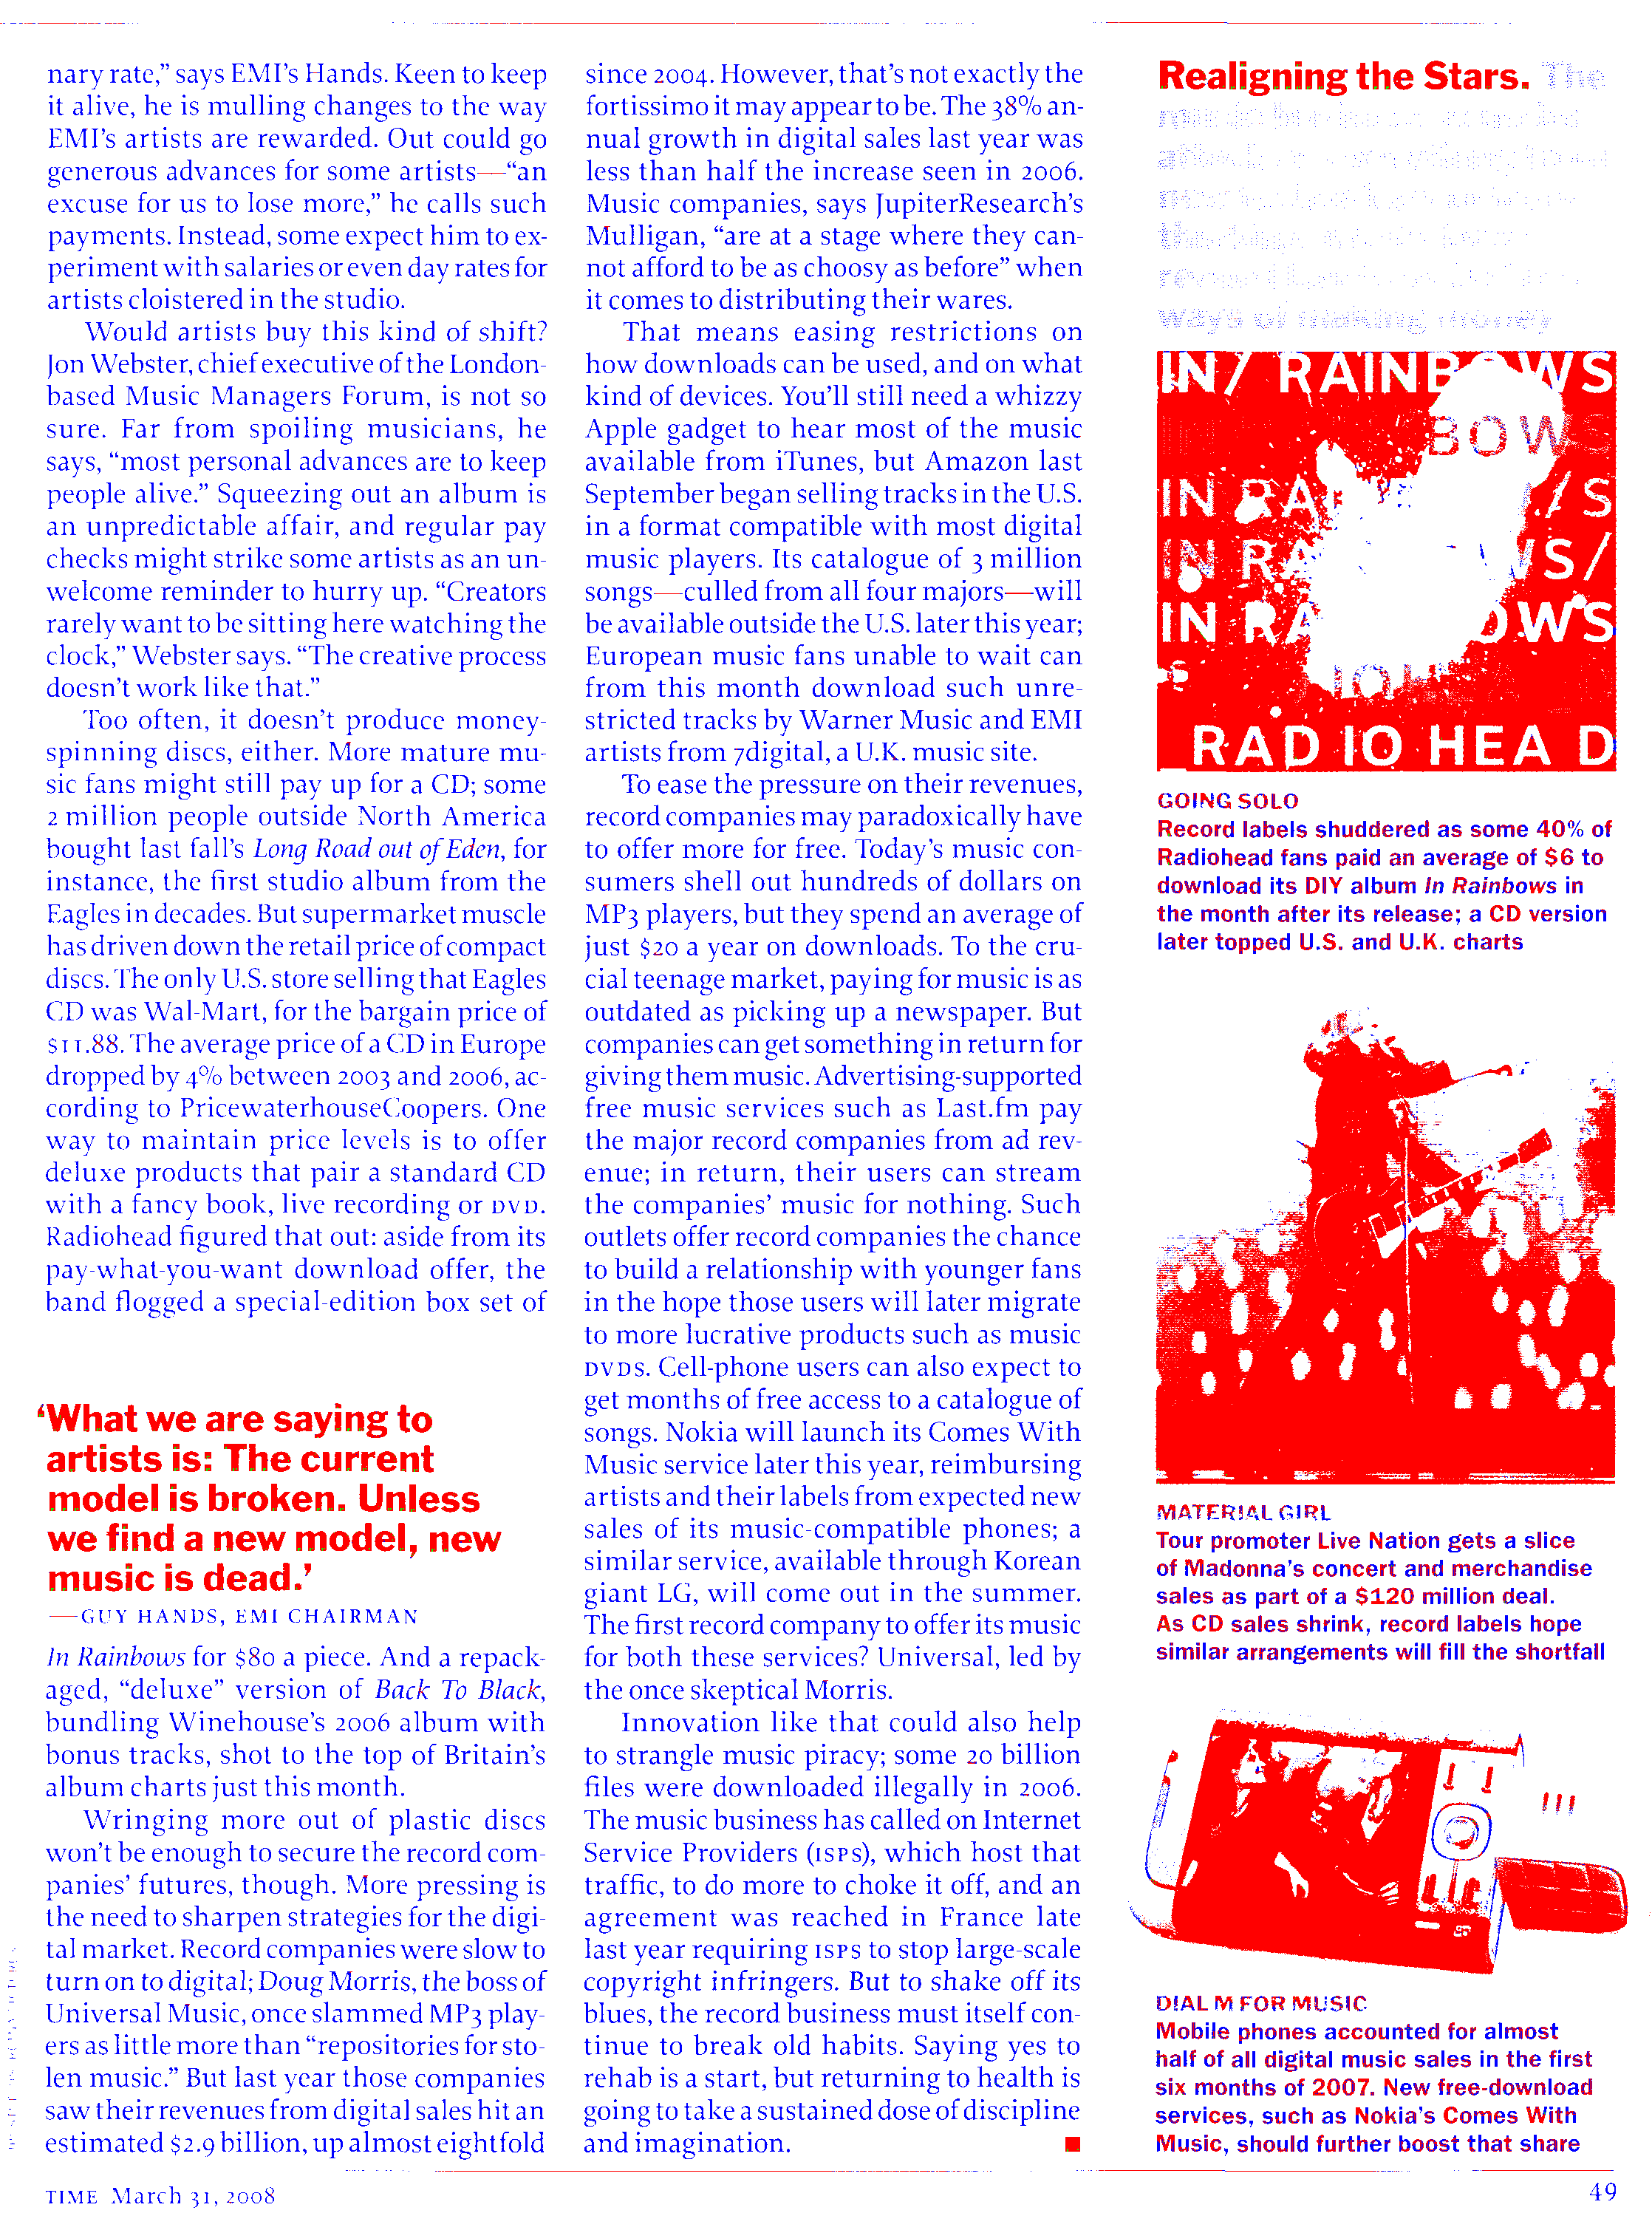
\includegraphics[width=0.4\textwidth]{assets/result_imagens/time_50_percent_sparse_9x9_785_final.png}
        \end{tabular}
      \end{center}
      \label{tab:segmentation_785}
    \end{table}
    \begin{table}[p]
      \caption{Segmentação da imagem 786}
      \begin{center}
        \begin{tabular}{ c c }
          Ideal & Segmentada \\
          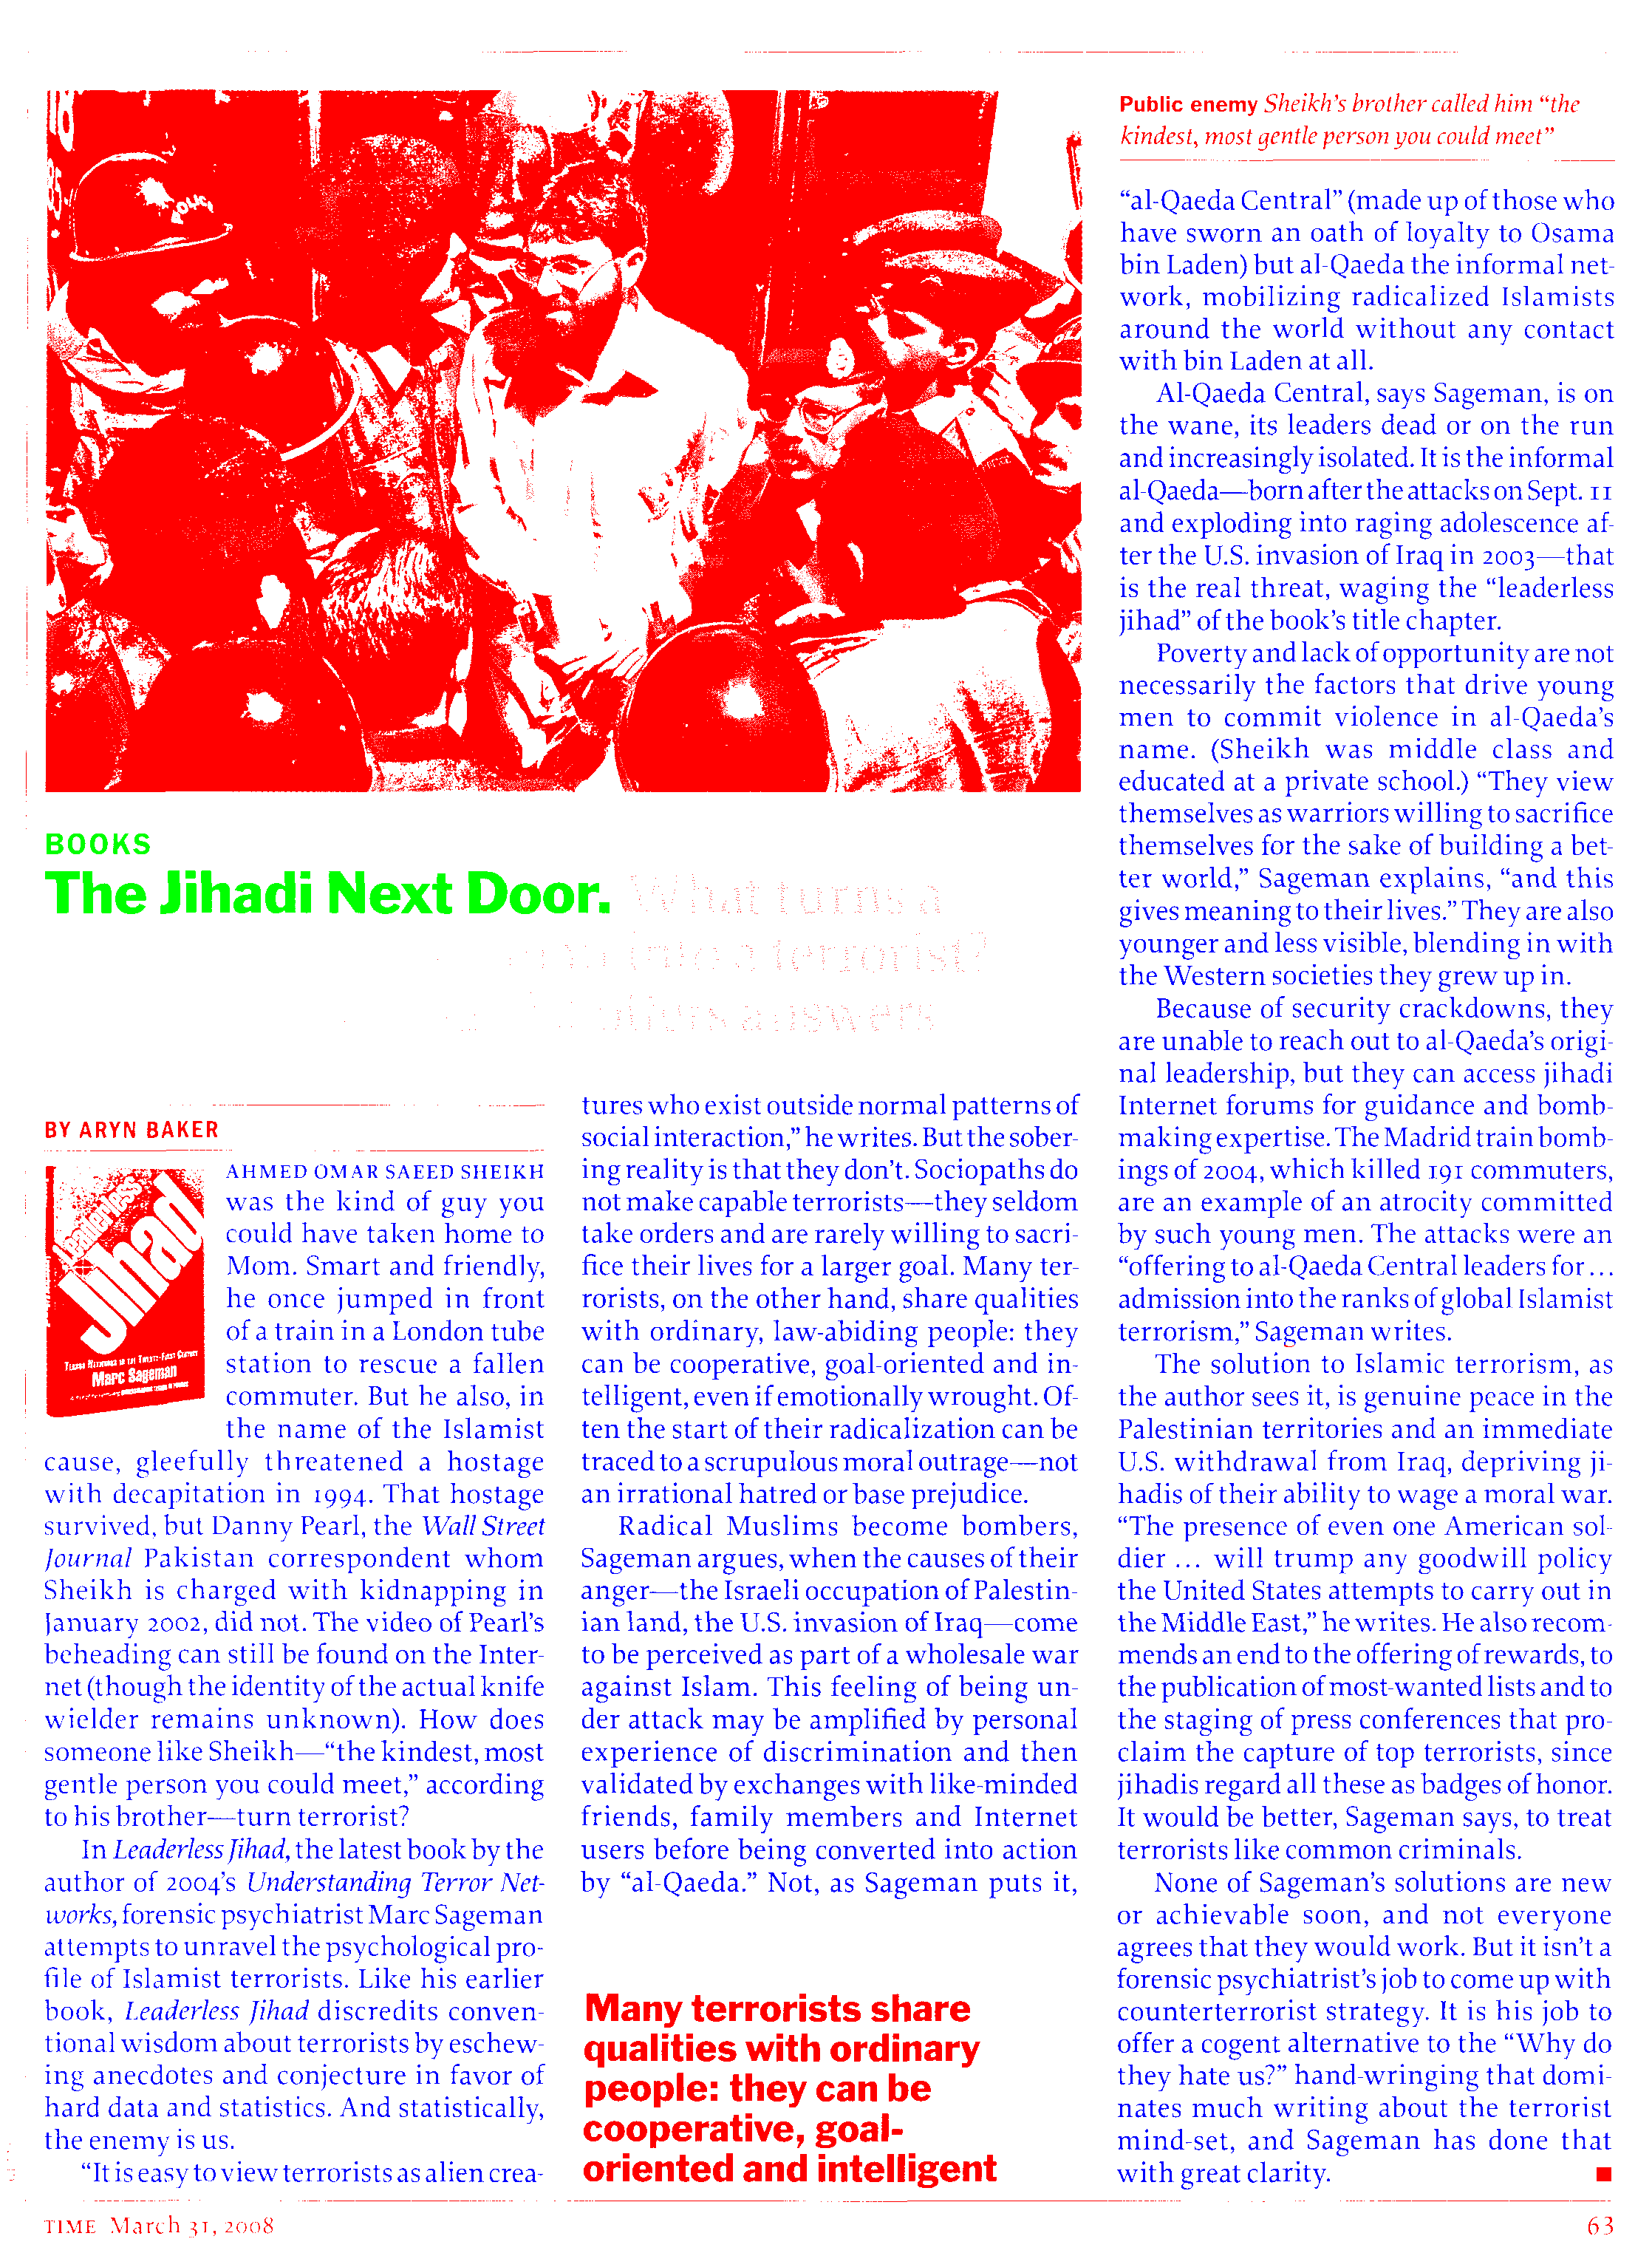
\includegraphics[width=0.4\textwidth]{assets/final_ideal/time_786_ideal.png}
          &
          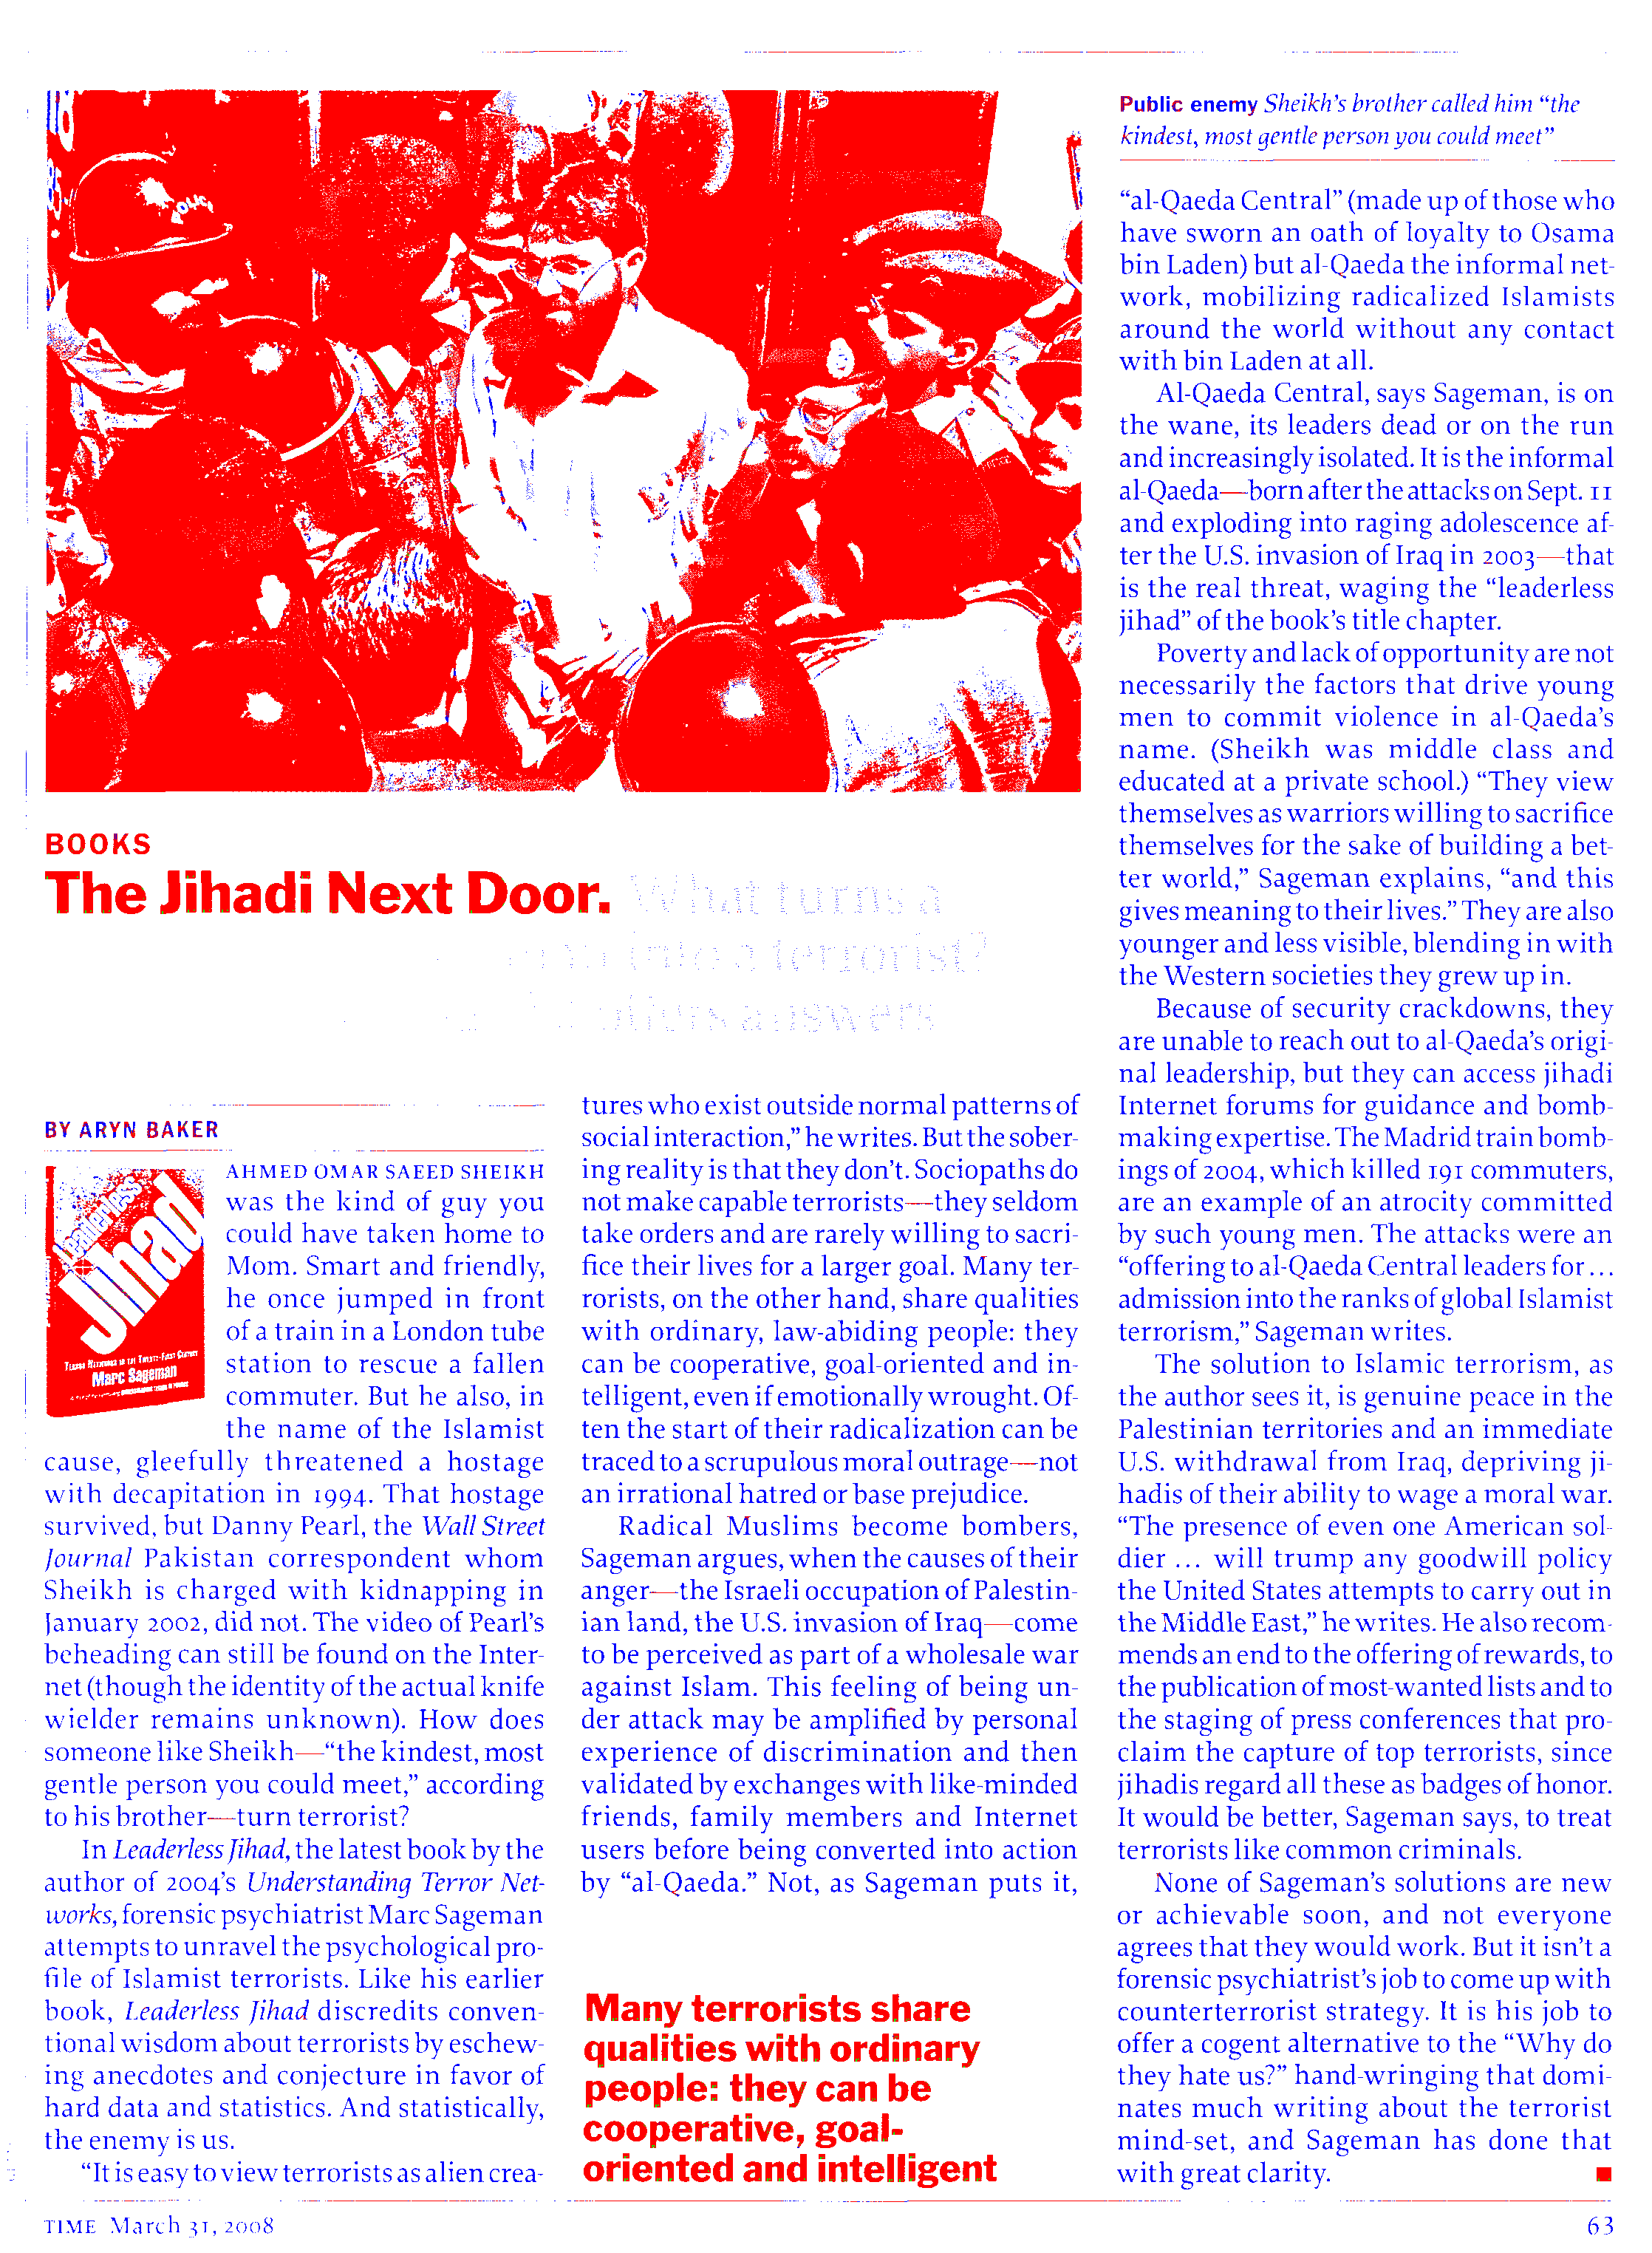
\includegraphics[width=0.4\textwidth]{assets/result_imagens/time_50_percent_sparse_9x9_786_final.png}
        \end{tabular}
      \end{center}
      \label{tab:segmentation_786}
    \end{table}

\clearpage

\section{Conclusão}
\label{sec:conclusao}

  Observamos comportamentos diferentes na classificação de parágrafos e títulos. A quantidade de imagens demonstrou-se menos relevante na classificação parágrafos do que na classificação de títulos. Isto se deve a maior quantidade de exemplos por página de texto de parágrafo do que de títulos.

  O tamanho da janela é o fator mais sensível, tanto para a qualidade quanto para o tempo de processamento. Janelas maiores porém esparsas apresentaram os melhores resultados, sendo o melhor deles observado para janelas 9x9 esparsas, atingindo F-measure de 0,96 para CACM e 0,93 para a TIME.

  Porém nem sempre a maior janela produz o melhor resultado. As janelas 11x11 desempenharam pior que as 9x9. Quanto maior a janela, mais exemplos são necessários. Podemos ver que em janelas maiores o tamanho do conjunto de treinamento possui maior influência na qualidade. Com janelas até 5x5 a quantidade de exemplos quase não altera a qualidade ou até piora.

  Exemplos ruins também podem comprometer a qualidade do operador. Fontes muito parecidas para títulos e outros tipos de texto podem fornecer exemplos contraditórios, ou seja, hora um certo padrão consta como título hora não. Podemos ver um exemplo deste fenômeno na imagem \ref{tab:segmentation_695} onde o texto à direita foi classificado como título por possuir características de título. Parte do motivo por este problema ocorrer é decorrente da decisão de testarmos apenas dois tipos de região (parágrafo e título). Possivelmente, caso tivéssemos classificados outros tipos de texto, poderíamos obter resultados melhores na etapa de consensualização.

  Uma outra possível melhoria seria trabalhar com imagens redimensionadas (reduzidas), fazendo com que os títulos ficassem menores, cabendo melhor dentro das janelas utilizadas.

  Não pudemos testar janelas maiores que 11x11 pois o tempo de processamento cresce muito rapidamente tornando o processo muito custoso.

  A comparação com outros métodos foi comprometida pela escolha das regiões a serem segmentadas. No artigo \cite{DBLP:conf/icdar/2009} vemos os resultados dos principais métodos para textos em geral e não parágrafos e títulos separadamente. Um outro problema é o método para avaliação, que utiliza polígono isotéticos, como proposto no artigo \cite{10.1109/ICDAR.2007.207}. Teríamos que realizar algum tipo de transformação que definiria polígonos em torno dos pixeis de uma certa região, assim como fez o método descrito em \cite{Moll07documentcontent}.

  Acreditamos que o método proposto pode ser empregado na extração de texto de documentos. Porém, diversos ajustes de otimização seriam necessários para criar uma ferramenta utilizável em situações práticas. O treinamento dos operadores é muito lento e aplicação também.

\section{Apêndice}

  \subsection{Algoritmo de Otsu para binarização}
  \label{sec:otsu}

    Implementar e avaliar cada algoritmo binarizador vai além do escopo deste trabalho, portanto escolhemos um bom algoritmo segundo os resultados obtidos em \cite{citeulike:890354}. Como o próprio artigo aponta, não foi encontrado um método que apresentasse desempenho superior em todas os cenários de teste realizados.

    Os requisitos para a escolha foram o da independência de supervisionamento e parametrização. Caso o algoritmo demandasse ajustes específicos de acordo com a imagem, o seu uso comprometeria a promissa de automatização. Dentre a lista de soluções com esta característica, escolhemos o algoritmo de Otsu \cite{1979:ots}, por ser de fácil implementação e apresentar resultados satisfatórios nos experimentos realizados.

    O algoritmo de Otsu encontra um nível de cinza $t$ tal que a soma ponderada da variância dentro das classes $\mathbb{F} = \{ x \colon f(x) \geq t \}$ (foreground) e $\mathbb{B} = \{ x \colon f(x) < t \}$ (background) seja minimizada, ou seja,

    \begin{equation}
      t = argmin \{ w_\mathbb{B} \sigma^{2}_{\mathbb{B}} + w_\mathbb{F} \sigma^{2}_{\mathbb{F}} \}
    \end{equation}

    onde $w_\mathbb{B} = \frac{|\mathbb{B}|}{|E|}$ e $w_f = \frac{|\mathbb{F}|}{|E|}$ são os pesos respectivamente do background e foreground e $\sigma^{2}_{\mathbb{B}}$ e $\sigma^{2}_{\mathbb{F}}$ são as variâncias das classes.

    A tabela \ref{tab:otsu} apresenta um passo a passo do algoritmo aplicado à figura \ref{fig:letrah}.

    
    \begin{table}[ht]
      \begin{center}
        \caption{Imagem original em escala de cinza e correspondente binarizada com $t = 50\%.$}
        \begin{tabular}{ c c }
            
\includegraphics[width=0.3\textwidth]{assets/binarization/h_3grayscale_big.png}
            \label{fig:letrah}
            &
            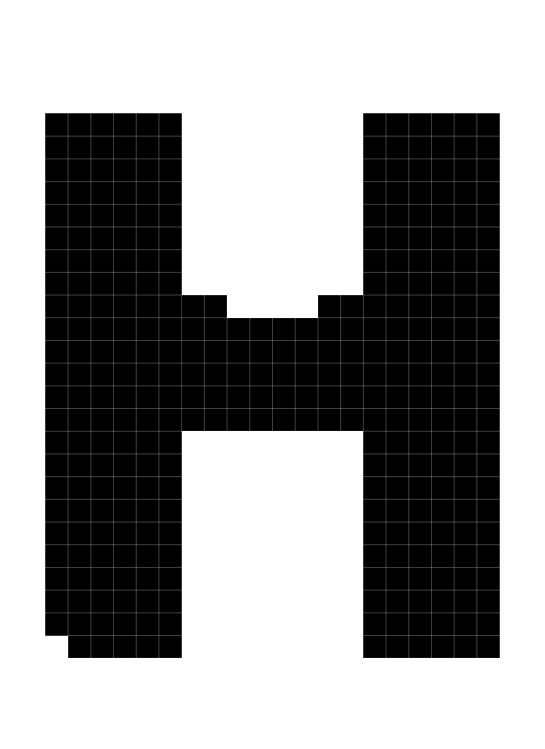
\includegraphics[width=0.3\textwidth]{assets/binarization/bin_big.png}
            
            \label{fig:letrah_bin}
        \end{tabular}
      \end{center}
    \end{table}

    \begin{center}

    \begin{table}
      \caption{Estágios da execução do algoritmo de Otsu.}
      \begin{tabular}[p]{@{}ccccccc@{}}
        \centering

        original & 25\% & 37,5\% & 50\% & 62,5\% & 75\% & 87,5\% \\

        % Imagem original e respectivo histograma
        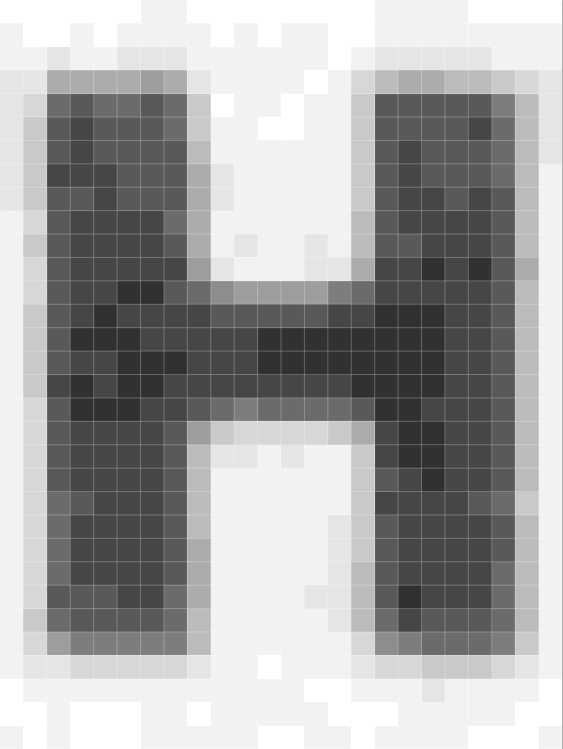
\includegraphics[width=0.05\textwidth]{assets/binarization/gray3_big.png}
        &
        
\includegraphics[width=0.05\textwidth]{assets/binarization/h25t.png}
        &
        \includegraphics[width=0.05\textwidth]{assets/binarization/h38t.png}
        &
        \includegraphics[width=0.05\textwidth]{assets/binarization/h50t.png}
        &
        \includegraphics[width=0.05\textwidth]{assets/binarization/h63t.png}
        &
        \includegraphics[width=0.05\textwidth]{assets/binarization/h75t.png}
        &
        \includegraphics[width=0.05\textwidth]{assets/binarization/h88t.png}
        \\

        % histogramas

        \includegraphics[scale=0.4]{assets/binarization/3bit_hist.png}
        &
        \includegraphics[scale=0.4]{assets/binarization/13hist.png}
        &
        \includegraphics[scale=0.4]{assets/binarization/25hist.png}
        &
        \includegraphics[scale=0.4]{assets/binarization/50hist.png}
        &
        \includegraphics[scale=0.4]{assets/binarization/63hist.png}
        &
        \includegraphics[scale=0.4]{assets/binarization/75hist.png}
        &
        \includegraphics[scale=0.4]{assets/binarization/88hist.png}

        \\
        % peso do background
        $w_\mathbb{B}$ & 0.1931 & 0.4015 & 0.4179 & 0.4532 & 0.5479 & 0.6969 \\

        % média do background
        $\mu_\mathbb{B}$ & 34.00 & 51.64 & 53.61 & 61.37 & 83.08 & 112.56 \\

        % variância do background
        $\sigma^{2}_{\mathbb{B}}$ & 7.27 & 288.58 & 372.94 & 1054.08 & 3128.03 & 5656.37 \\

        % peso do foreground
        $w_{\mathbb{F}}$ & 0.80 & 0.59 & 0.58 & 0.54 & 0.45 & 0.30 \\

        % média do foreground
        $\mu_{\mathbb{F}}$ & 184.87 & 225.55 & 229.03 & 233.95 & 243.79 & 255.0 \\

        % variância do foreground
        $\sigma^{2}_{\mathbb{F}}$ & 5799.89 & 1409.01 & 1006.11 & 673.10 & 255.43 & 0.0 \\

        % variância intra-classe
        $\sigma^{2}_{w}$ & 21495165144 & 967521582 & 512693389 & 595067475 & 4269882800 & 17660993341 \\

        \label{tab:otsu}
      \end{tabular}
    \end{table}
    \end{center}

    Como podemos notar, para $t = 50\%$ atingimos o menor valor de $\sigma^{2}_{w} \approx 512693389$. Neste caso o limiar coincide com o único vale no histograma, porém isto nem sempre será válido. Algumas imagens não possuem vales bem definidos. Este algoritmo não se baseia no formato do histograma mas sim na coesão intra classe e na separabilidade das classes.

    Uma desvantagem de utilizar este algoritmo é a influência da média de todo os pixeis da imagem. Isto pode fazer com que o limiar ótimo para a página toda não seja o mesmo que o de dentro de uma janela.

    \subsection{Implementação}

    Todos os experimentos foram realizados utilizando scripts ruby e python para automatizar a tarefa. Também utilizamos a biblioteca ImageMagick e bibliotecas para manipulação de XML.

    O processo todo consistiu em baixar a base de dados do PRImA, processá-las gerando as entradas para o TRIOS, construir os operadores, aplicá-los, consensualizar e extrair métricas.

    Este trabalho tem como objetivo provar um conceito: avaliar a aplicabilidade de operadores morfológicos à segmentação de página. Logo o código gerado não é destino a aplicações comerciais.

    \begin{itemize}
      \item sample\_generator.rb produz todos os conjuntos de imagens para treinamento e teste, ou seja, ele transforma todas as imagens e XMLs da base de dados original em entradas apropriadas para as ferramentas que utilizamos.
      \item imgset\_training\_gen.rb gera e aplica todos os 200 operadores utilizados nos experimentos. Utiliza os executáveis trios\_build e trios\_apply fornecidos pelo TRIOS.
      \item measures.py extrai todas as estatísticas apresentadas na seção \ref{sec:resultados}.
      \item consensus.py faz a união das segmentações realizadas pelo apply\_all.rb
      \item merge.py cria imagens segmentadas coloridas para visualização.
    \end{itemize}


%\bibliographystyle{alpha}
{\small 
\bibliographystyle{unsrt} % (uses file "plain.bst")
\bibliography{myrefs}   % expects file "myrefs.bib"
}

\end{document}
